\section{--Topics for further investigation--}
\begin{itemize}
	\item Figure out the Notebook script. How to connect to the workspace, create an environment.
	\item Figure out, how to design own  repository (Service-Index) 
	\begin{itemize}
		\item to log metrics 
		\item to log results
		\item to attach the script, which was usesd for thrun.
		\item Contextualise Experiments
	\end{itemize}
	\item Create Neural Network in Azure ML Workspace (3Blue1Brown Anleitung)
	\item Go though the 3-Houre Coure to learn more about metrics and stuff.
\item LinkedIn Learning Couse
% Reference to LinkedInd Learning Course
%1. Introduction into ML
%2. Introduction int Azure ML
%3. Improving Azure ML Models
%4. Deployment and Monitoring of Models
%5. Interpreting Models: Model Drift, etc.
\end{itemize}

\begin{comment}
	
	\paragraph{Framework agnostic}
%TODO: OLD Unclear how to use it.
Over this platform 
\begin{itemize}
	\item Scikit-learn, 
	\item Tenserflow, 
	\item \gls{g_ONNX},
	\item MLFlow,
	\item PyTorch
\end{itemize}

\++section{Azure Machine Learning SDK}
Azure provides a \gls{SDK} for Python and \gls{R} to interact with the services of \gls{AML} in different enviorments.

\begin{figure}[H]
	\centering
	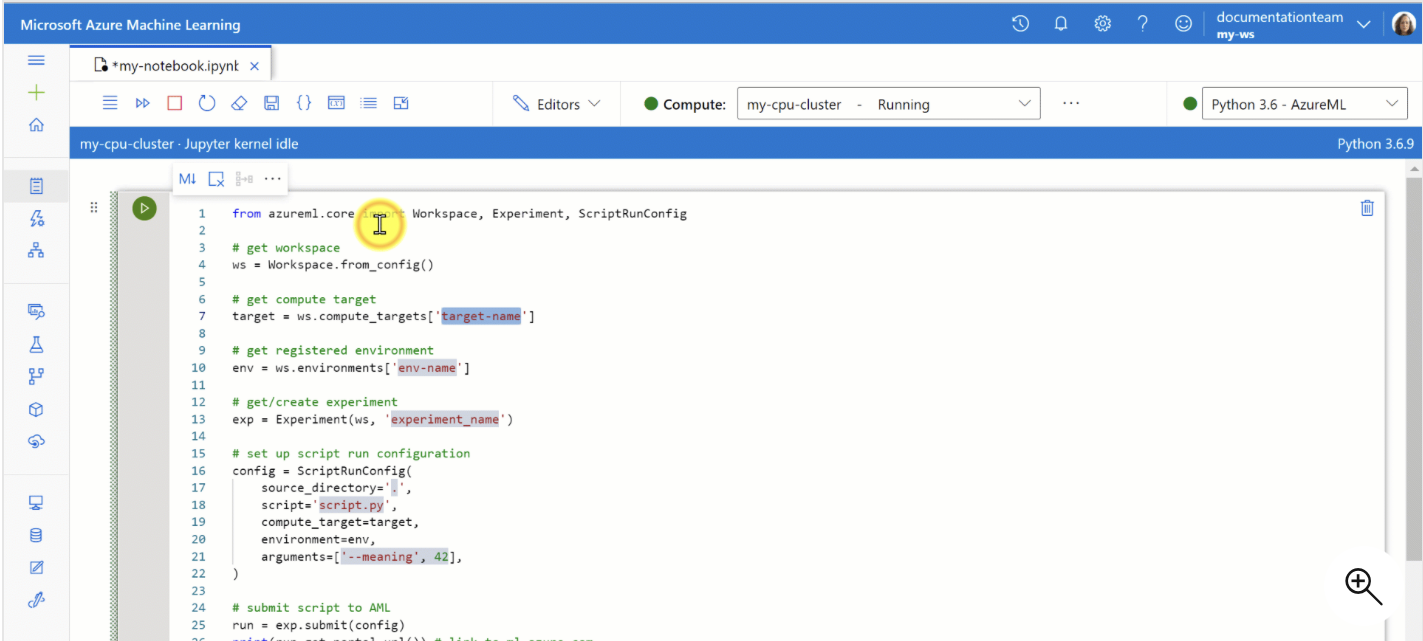
\includegraphics[scale = 0.4]{attachment/chapter_10/Scc003}
	\caption{Crt + Space - IntelSense}
\end{figure}

\end{comment}

\section{Platform Components}
%TODO: Hyperparametersation
% Understanding the --bath_size command
% And derive how to realy execute it

\subsection{AutoML}
Given a dataset to AutoML, it streamlines the process of finding the best model.\\

AutoML experiments with different \textit{features, algorithmes and hyperparameters}. The model can then by exported into \gls{g_ONNX} to be used on various platforms and devices. 

\begin{figure}[H]
	\centering
	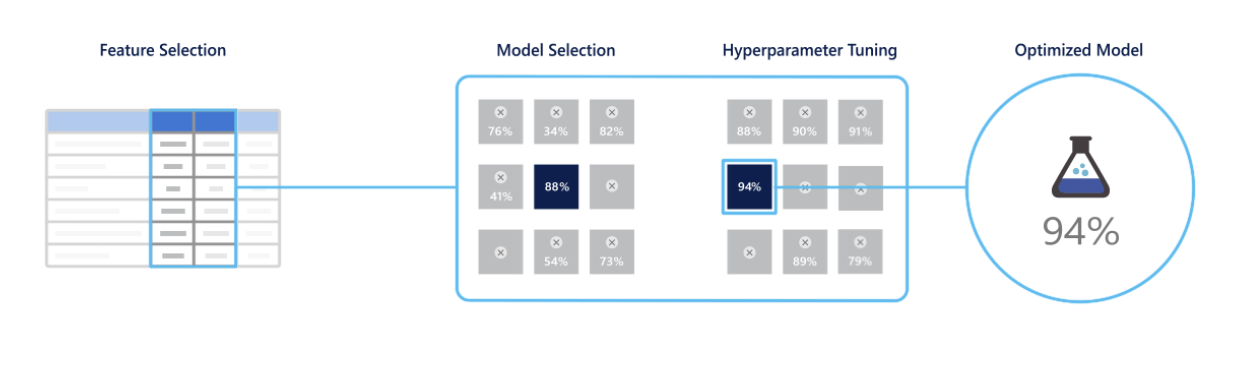
\includegraphics[scale = 0.4]{attachment/chapter_10/Scc004}
	\caption{AutoML Process}
\end{figure}

In the first step, for different Models different features will be tested. If the models scores well, then the hyperparametesation takes place. All the parameter, which goes into building the model will be tuned.

\subsection{Datasets}
The component \textit{Datasets} can be thought of as Linked Cloud Data sources and build-in data store.

\subsubsection{Linked Cloud Data Sources}

Because it is a Azure service many azure services can be linked to it. For example
\begin{itemize}
	\item Azure Data Lake
	\item Azure Blob Storage
	\item SQL Database
	\item Databricks File System
\end{itemize}

\begin{figure}[H]
	\centering
	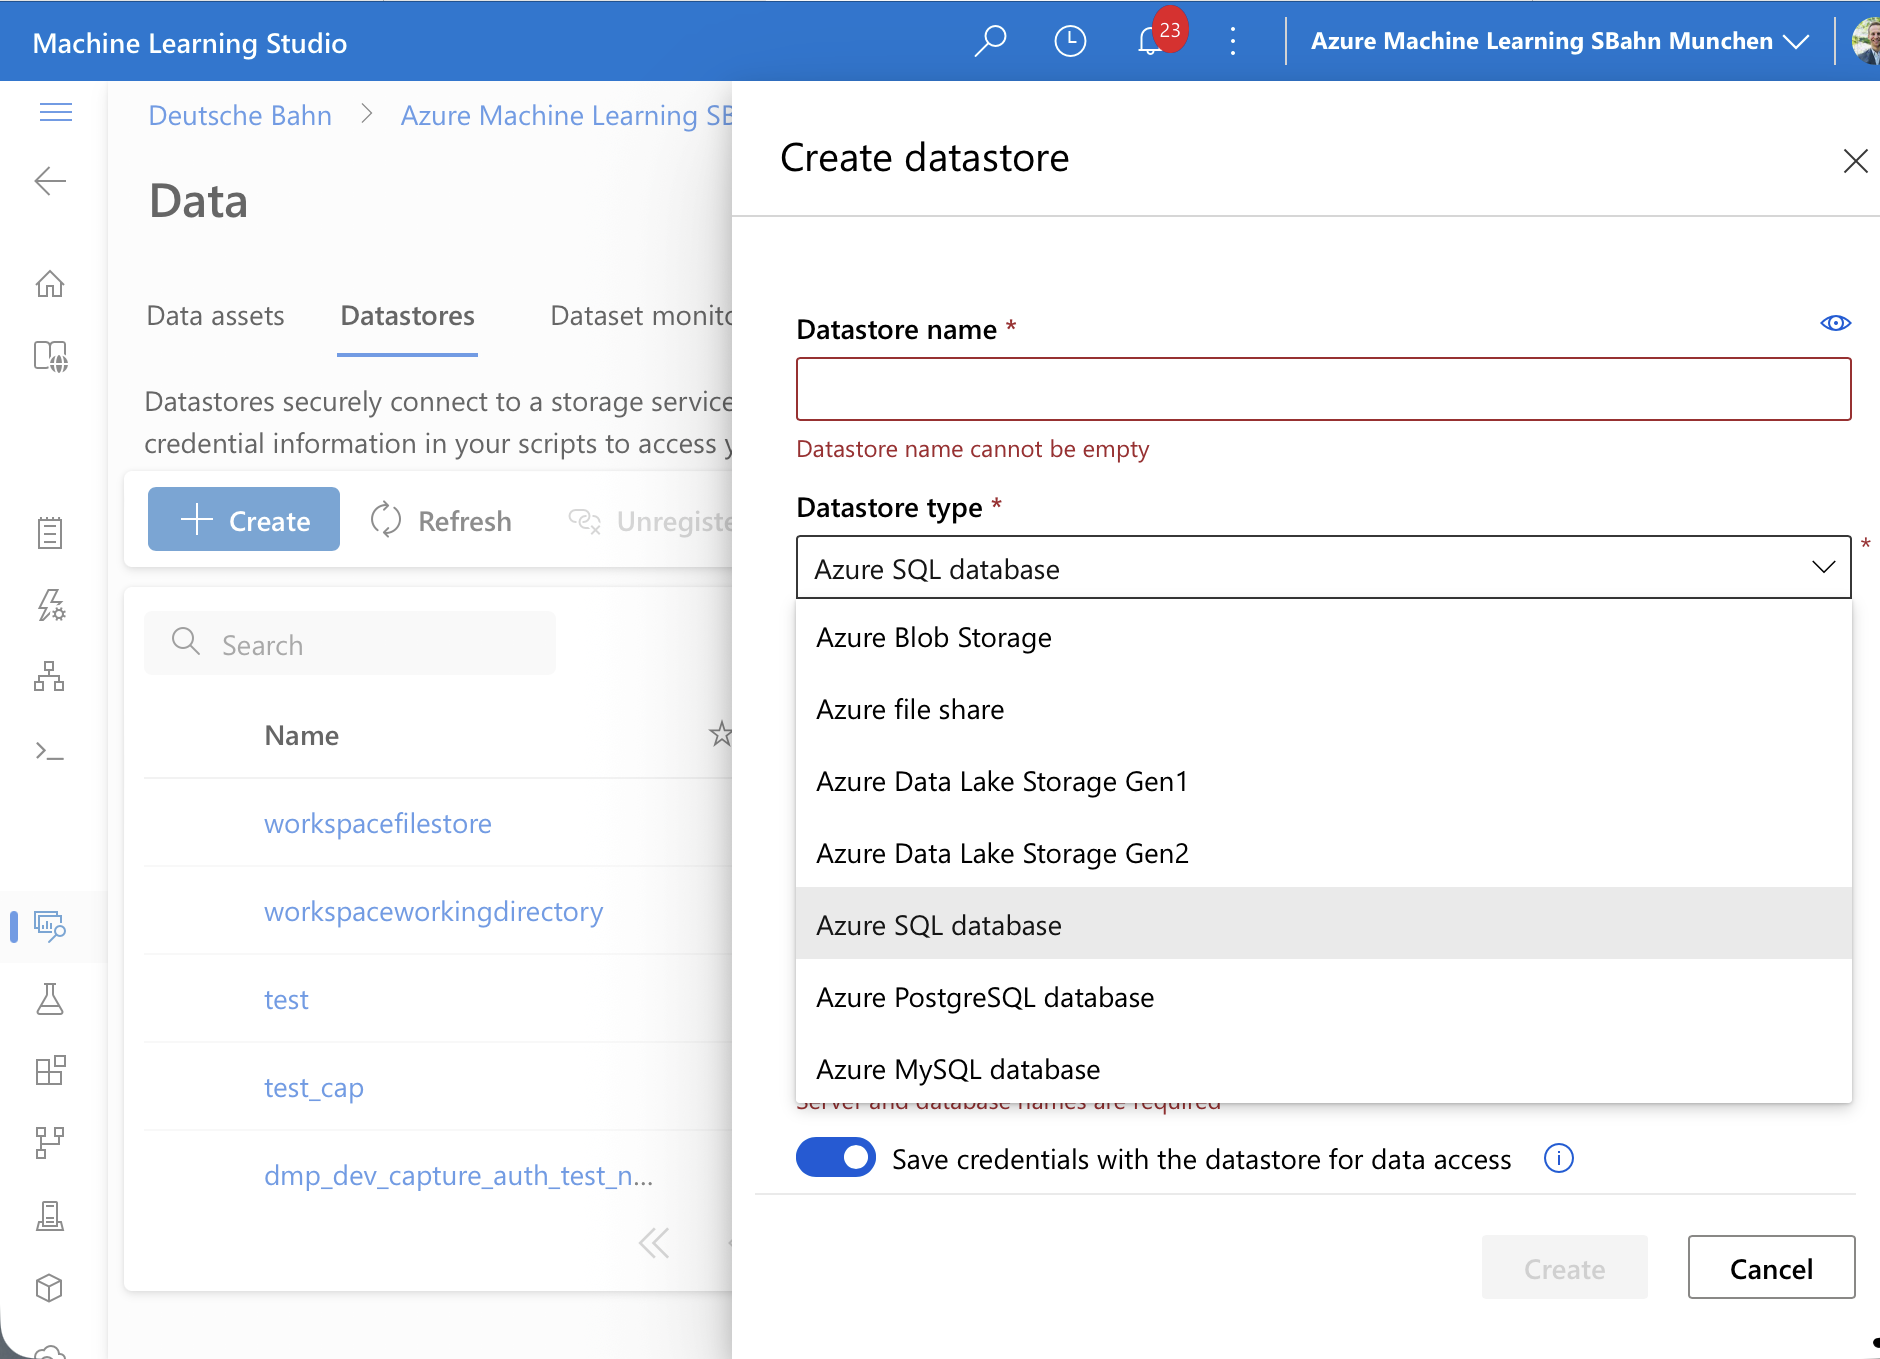
\includegraphics[scale = 0.2]{attachment/chapter_10/Scc028}
	\caption{Create a data storage connection}
\end{figure}

To note: Currently a link to a dedicated \gls{SQL} pool is not available. From those connection datasets are created.\\

A dataset can den be created from previous conneced datastore or from a local file or example registered datasets provided by \textit{Azure}.

\begin{figure}[H]
	\centering
	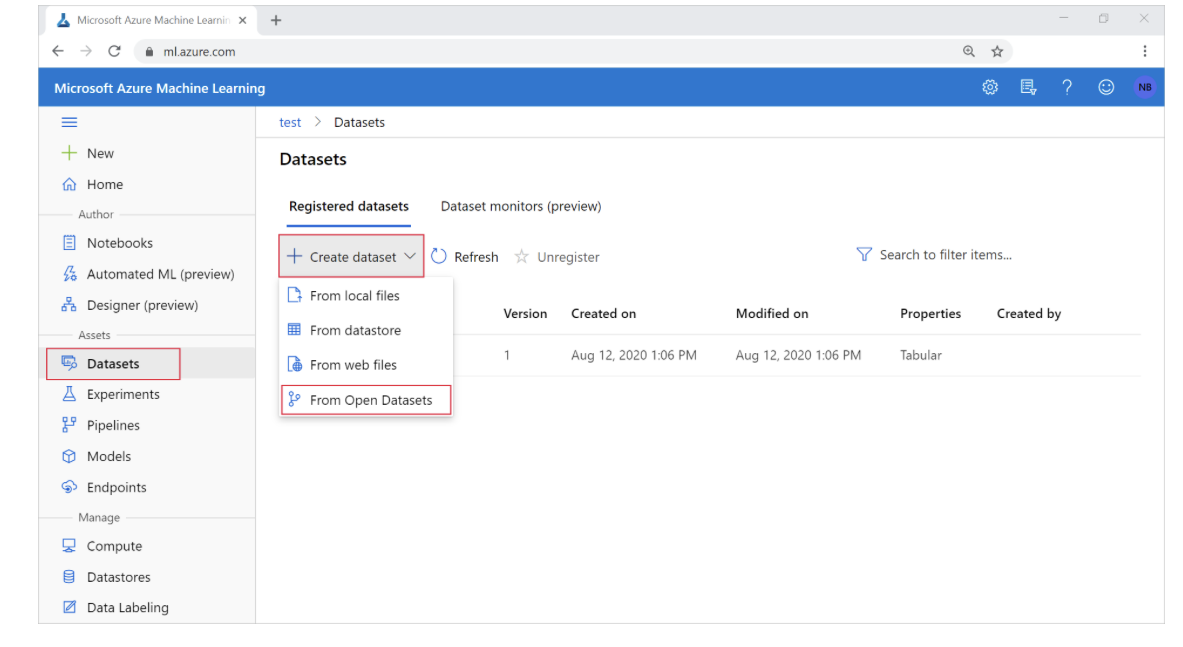
\includegraphics[scale = 0.2]{attachment/chapter_10/Scc006}\\ 
		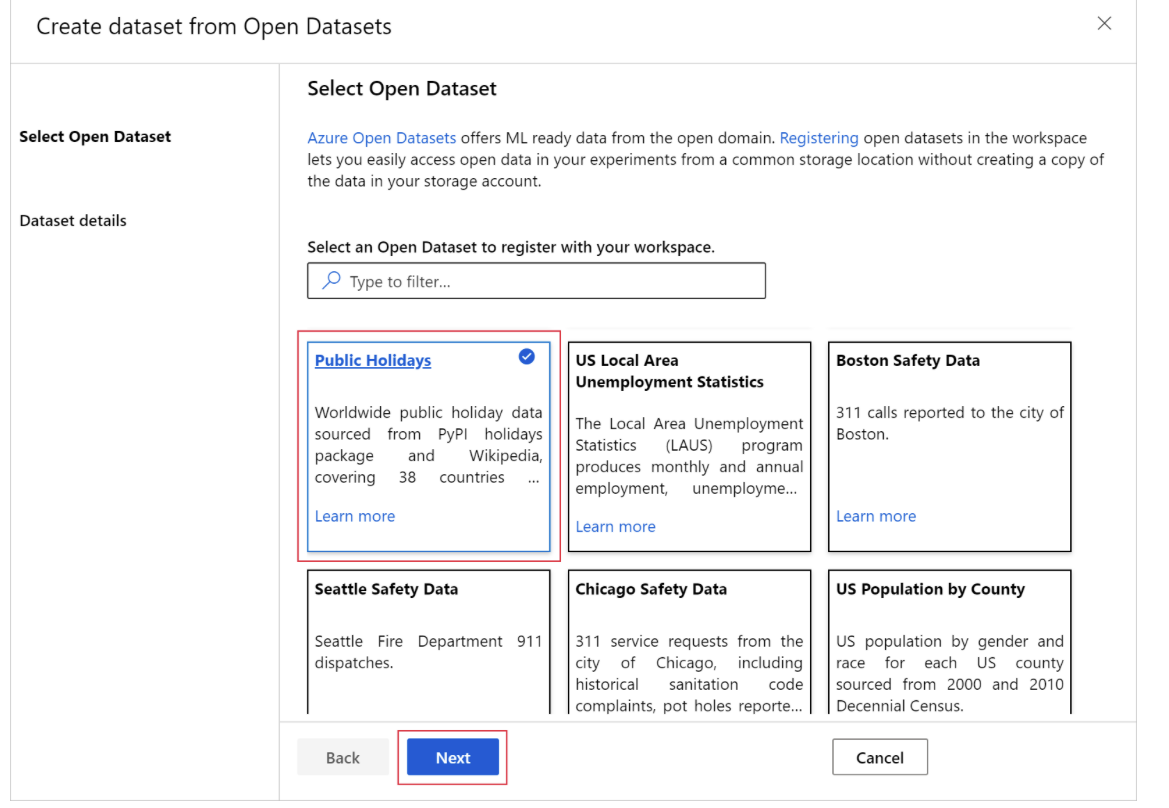
\includegraphics[scale = 0.2]{attachment/chapter_10/Scc007}
	\caption{Create a dataset}
\end{figure}

There are a variety of suppored data type 

\begin{figure}[H]
	\centering
	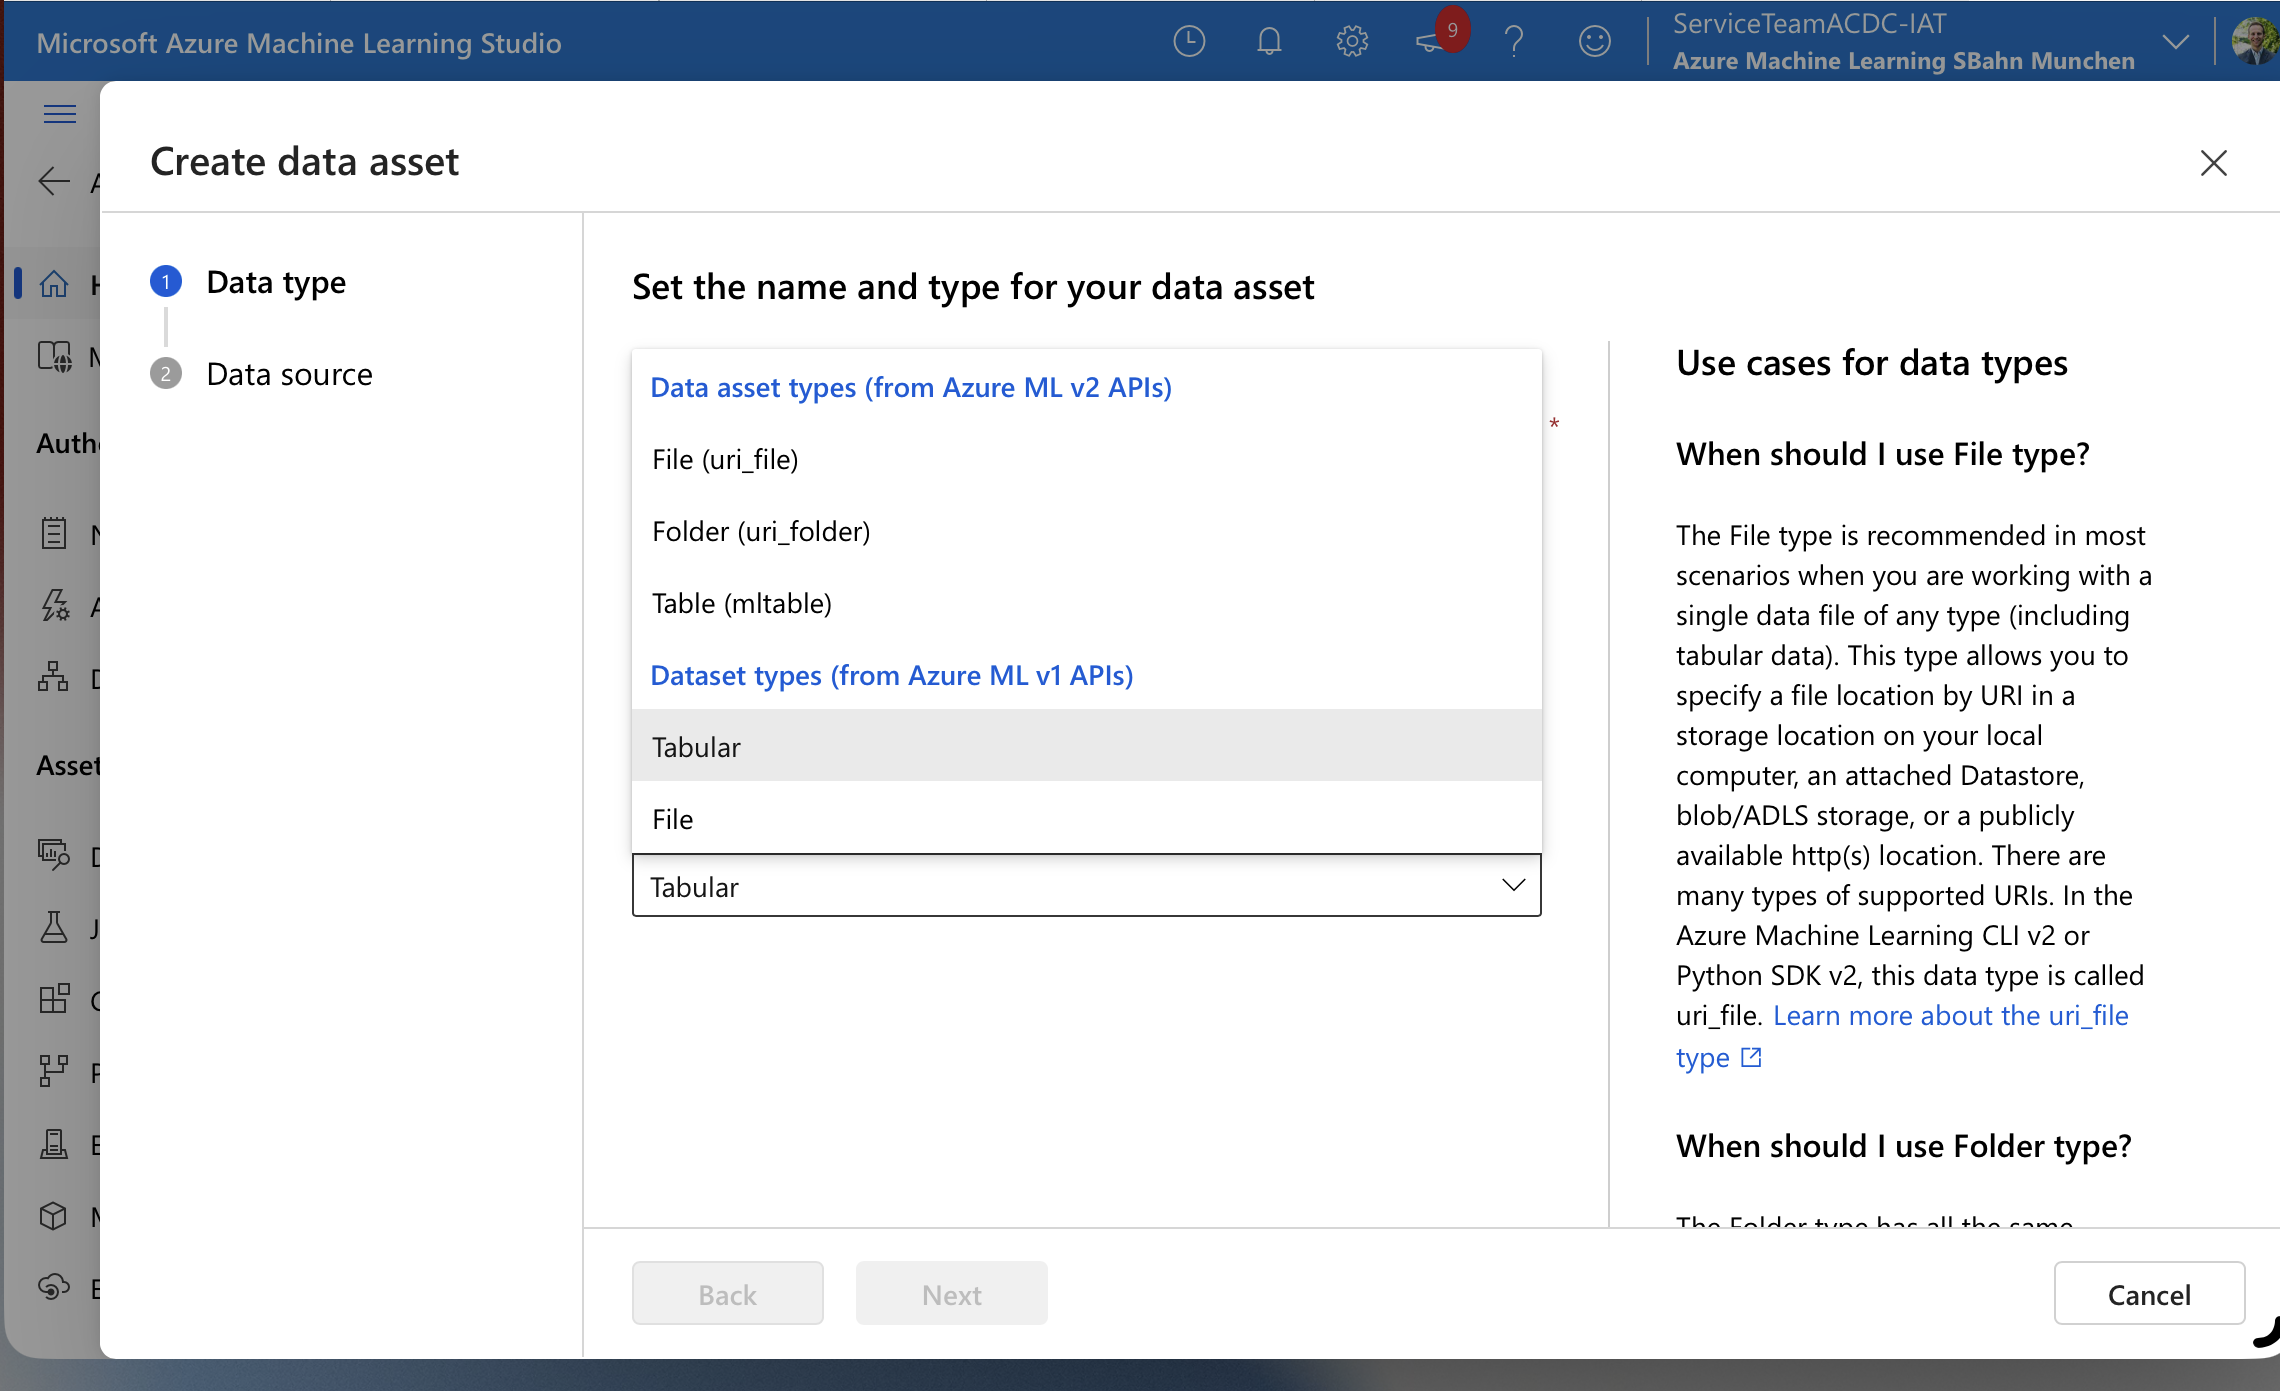
\includegraphics[scale = 0.1]{attachment/chapter_10/Scc008}
	\caption{New dataset types}
\end{figure}

A dataset can be 
\begin{itemize}
	\item registers, to allow others to work with it 
	\item versioned, to see the changes in the schema or data inside
\end{itemize}

In summery the dataset is a pointer to the datastore, where the data lifs.

\subsubsection{Build-in Data Store: Three Systems}
When you create a workspace, an Azure blob container and an Azure file share are automatically registered as datastores to the workspace.They're named \textit{workspaceblobstore} and \textit{workspacefilestore}, respectively. The workspaceblobstore is used to store \textbf{workspace artifacts} and your machine learning \textbf{experiment logs}. It's also set as the default datastore and can't be deleted from the workspace. The workspacefilestore is used to store \textbf{notebooks} and \textbf{R scripts} \underline{authorized via compute instance}.

\begin{lstlisting}[style=python]
import azureml.core
from azureml.core import Workspace, Datastore
     
ws = Workspace.from_config()	
\end{lstlisting}

\begin{figure}[H]
	\centering
	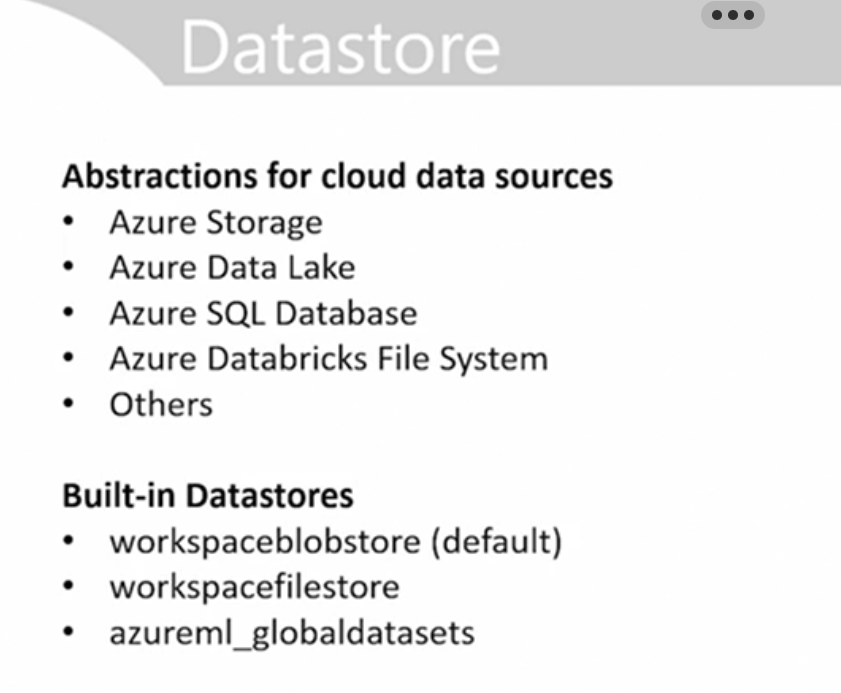
\includegraphics[scale = 0.3]{attachment/chapter_10/Scc029}
	\caption{Type of datasets}
\end{figure}

[!NOTE] Azure Machine Learning designer will create a datastore named \textit{azureml globaldatasets} automatically when you open a sample in the designer homepage. This datastore \textbf{only contains sample datasets} . Please do not use this datastore for any confidential data access.

\subsubsection{Example: Filestore}
In summery: Three workspace resources are created

	\begin{description}
		\centering
		\item[blobstore (default)] Artifacts of \gls{ML} Expermiments logs
		\item[filestore] Notebooks, Scripts
		\item[azureml globaldatasets]
	\end{description}

In the workspace this are further separated.

\begin{figure}[H]
	\centering
	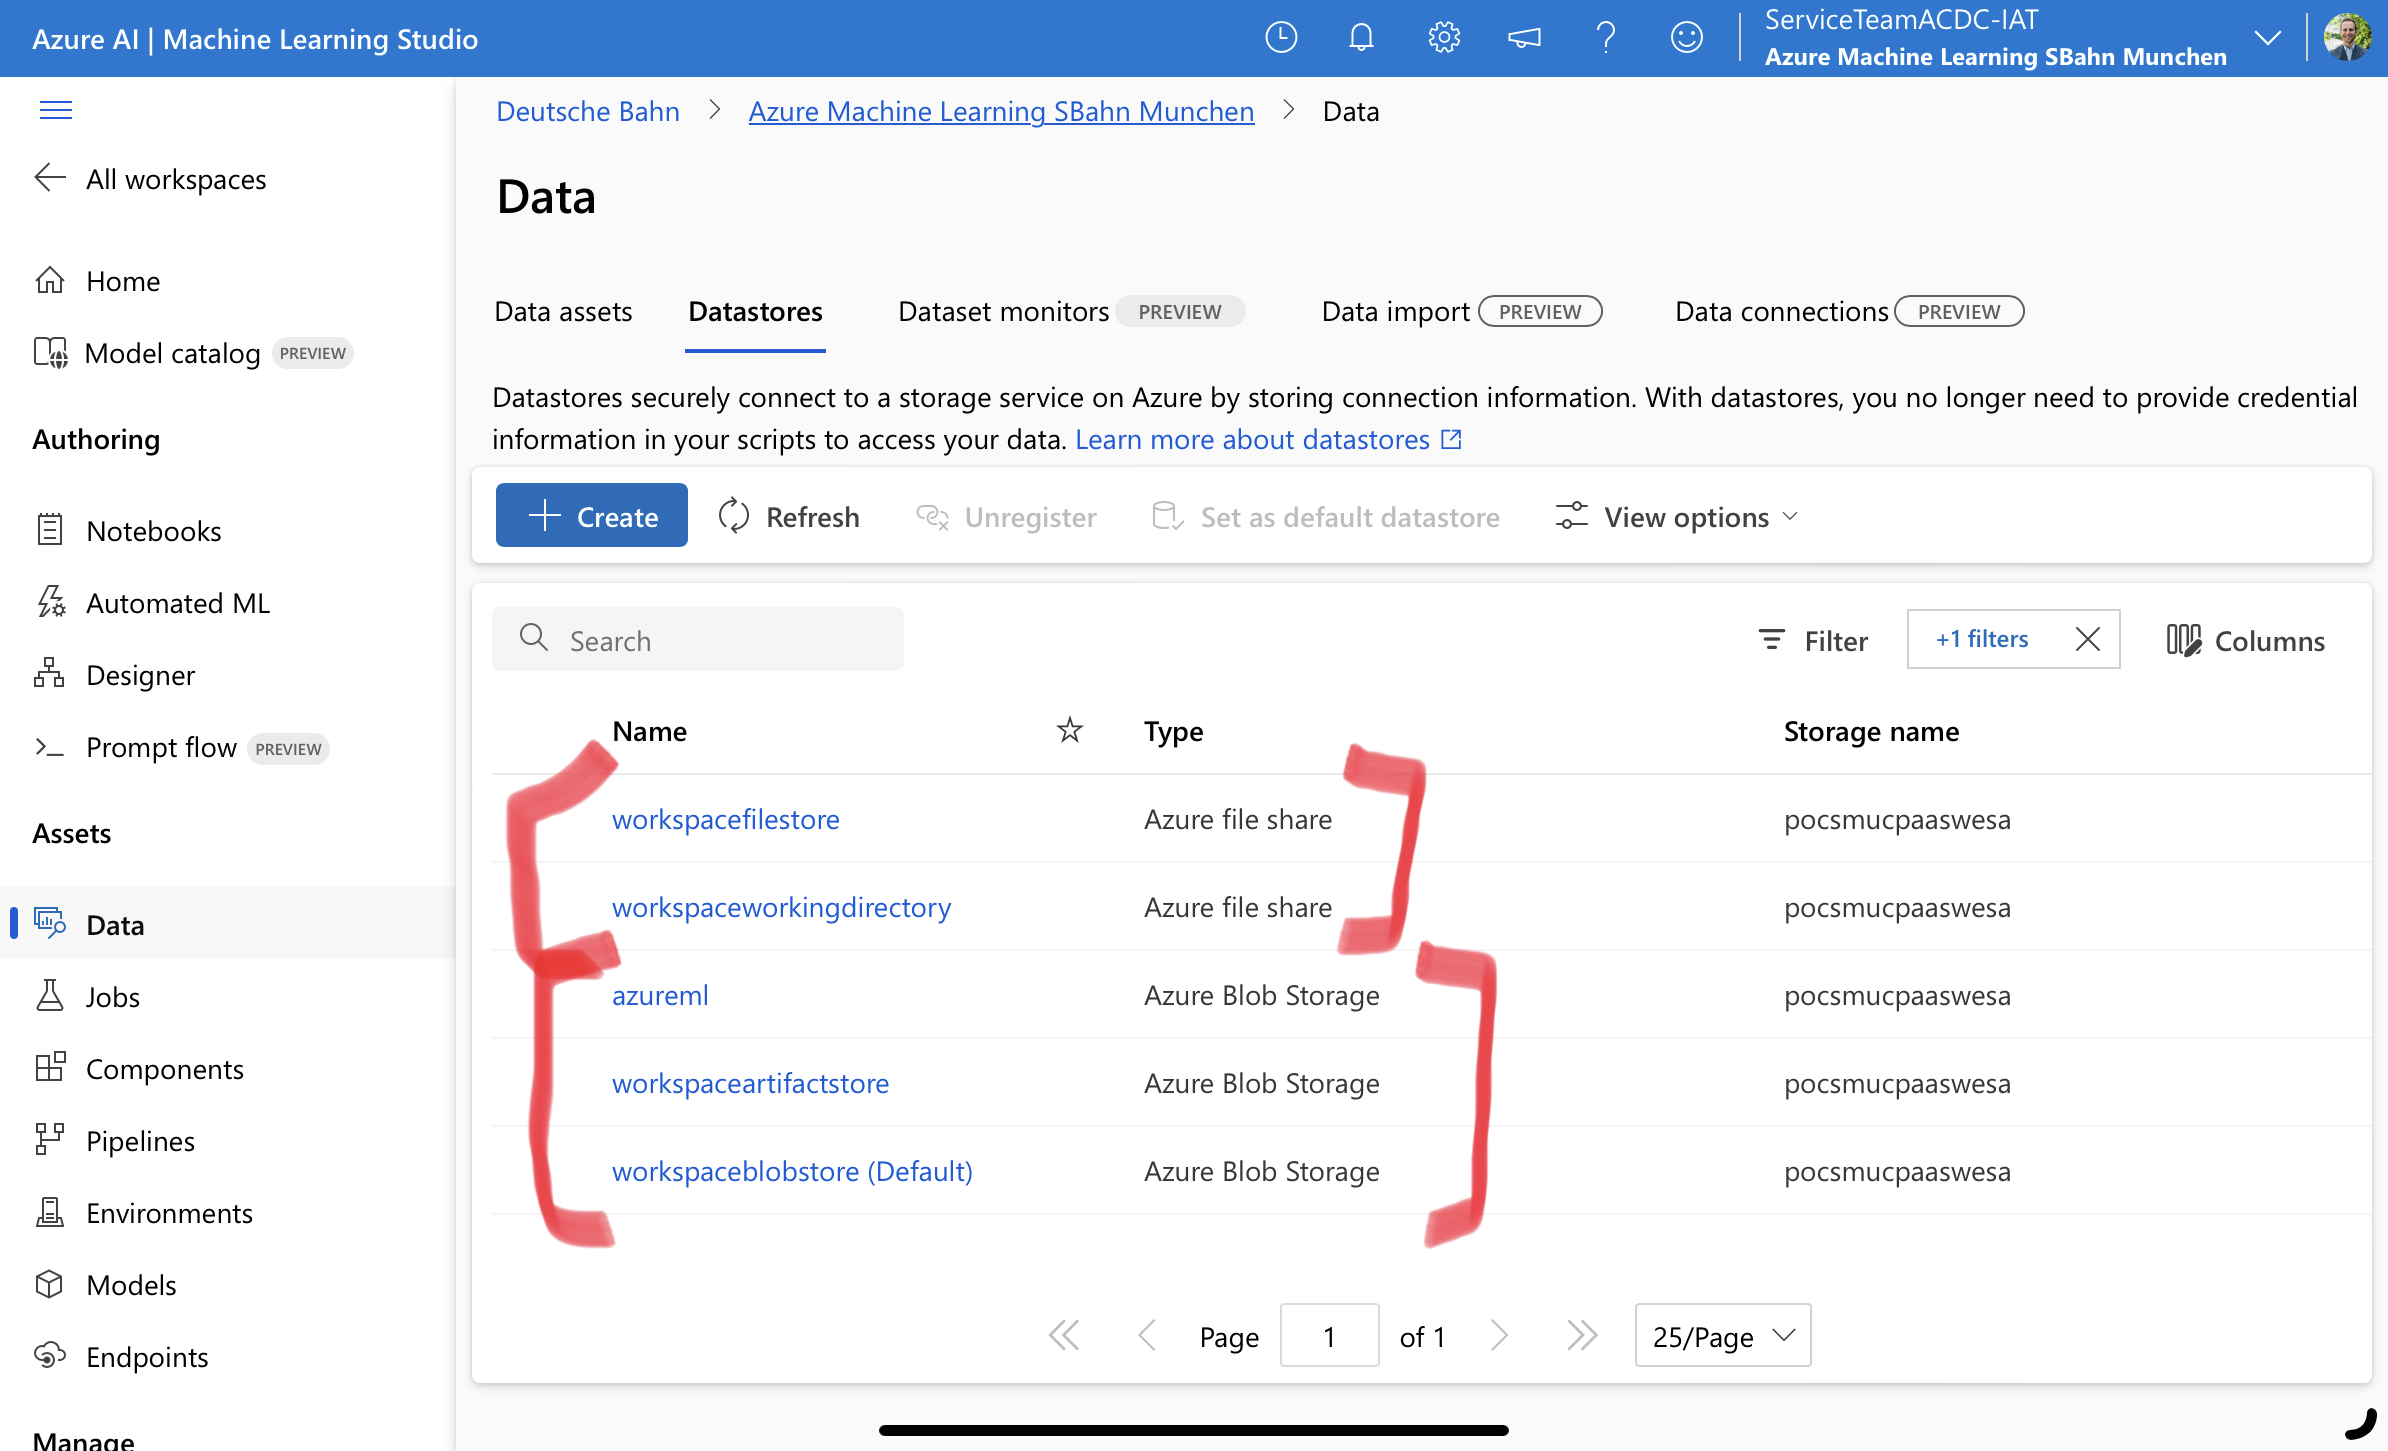
\includegraphics[scale = 0.1]{attachment/chapter_10/Scc036}
	\caption{Four seperate accounts: Two for file and for logs.}
\end{figure}

\begin{description}
	\item[workspacefilestore (filestore)] This account is normally reserved for notebooks and own created scripts. In this setup it is empty.
	\begin{figure}[H]
		\centering
		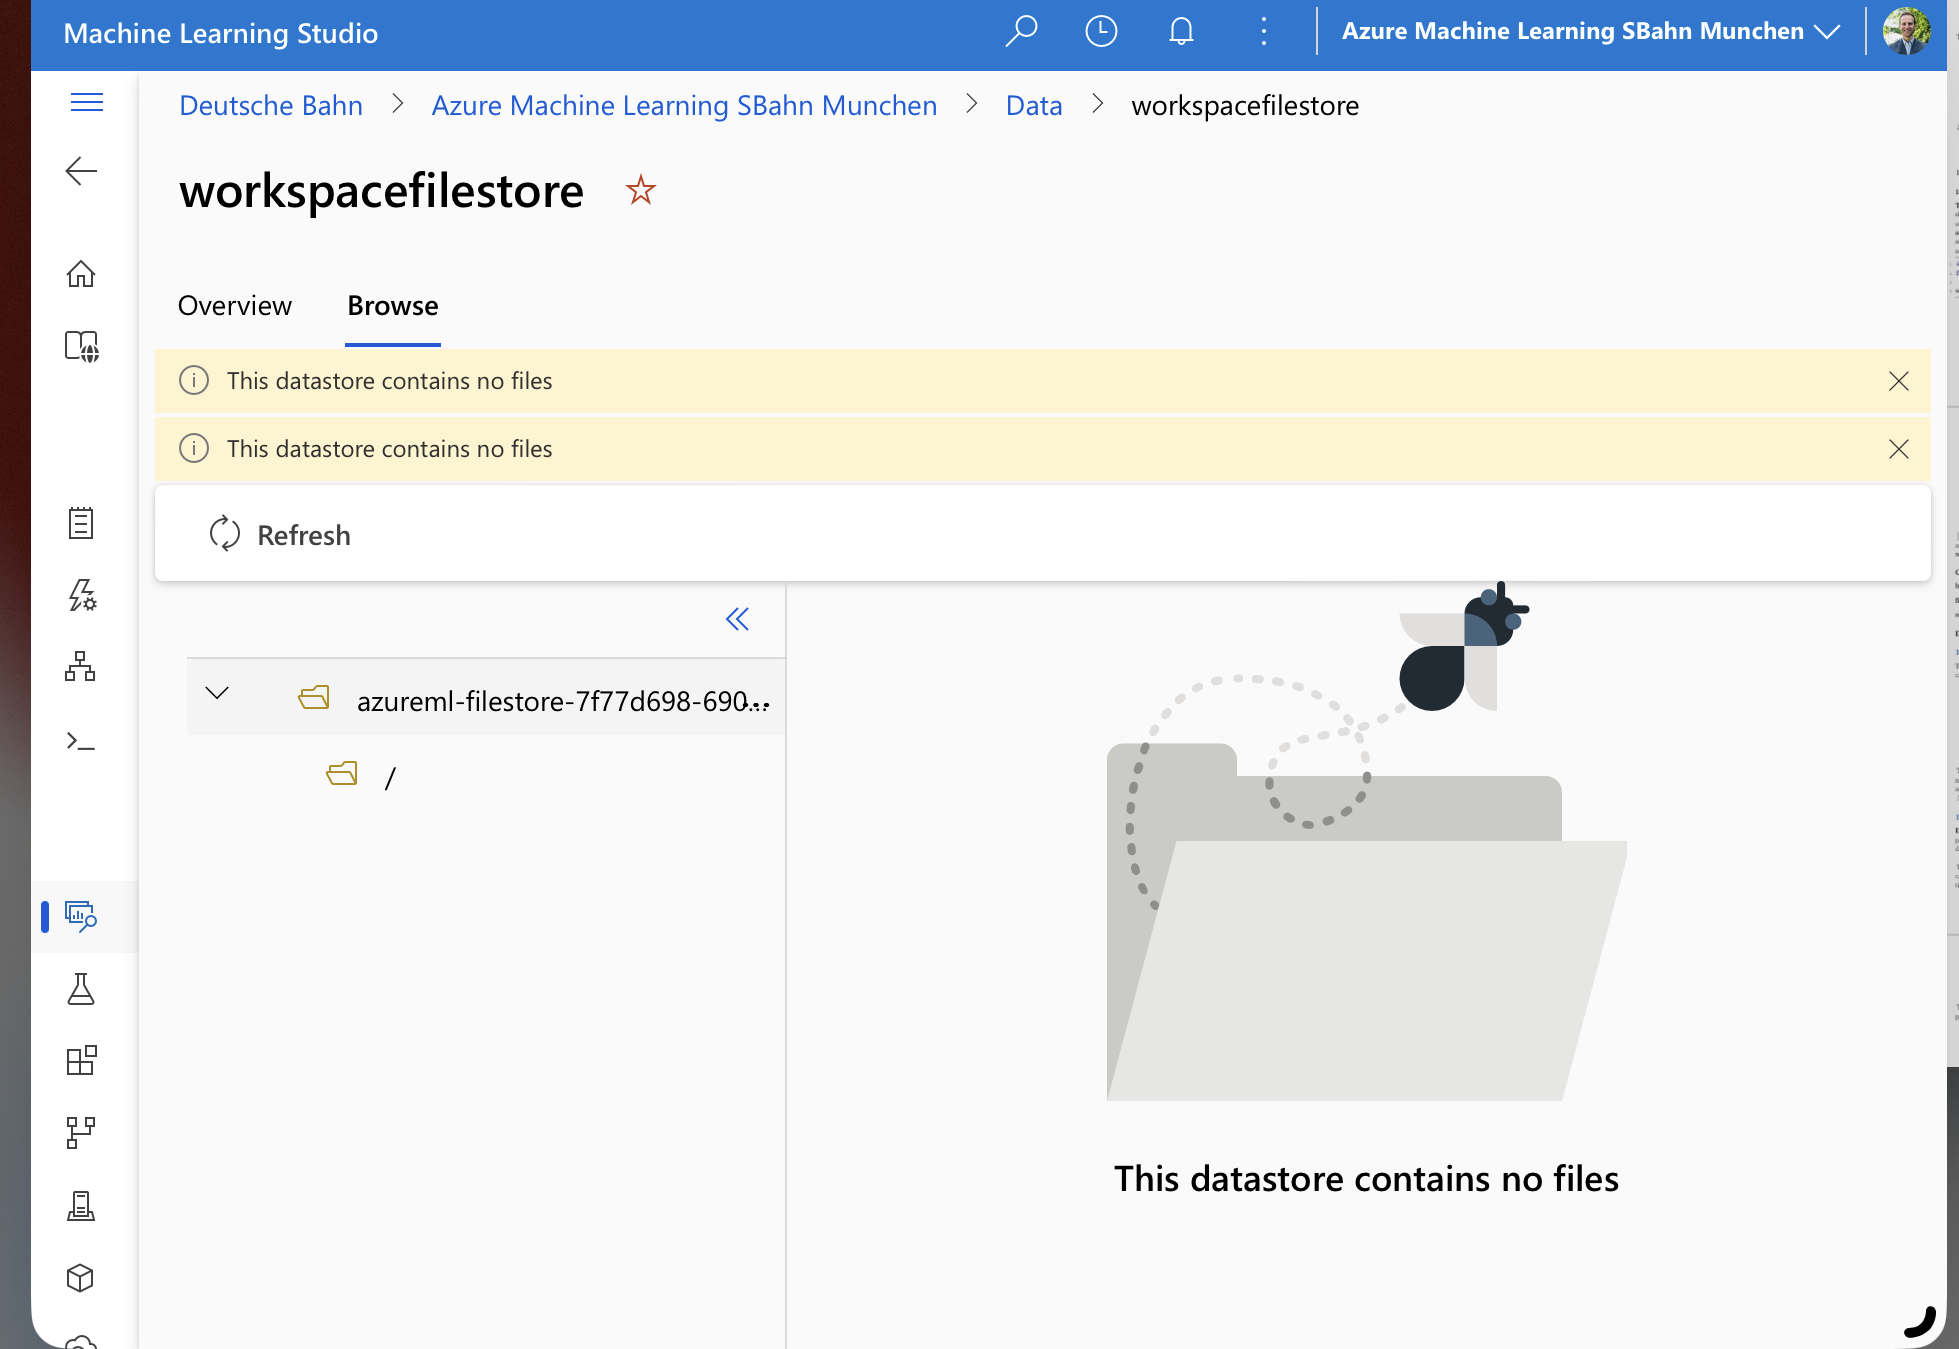
\includegraphics[scale = 0.1]{attachment/chapter_10/Scc037}
		\caption{In this setup it is empty.}
	\end{figure}
	\item[workspaceworkingdirectory (filestore)] Each user has it's own filesystem. Even each user get's created a own directly. Note: It is unclear, when exactly this happens. 
	\begin{figure}[H]
		\centering
		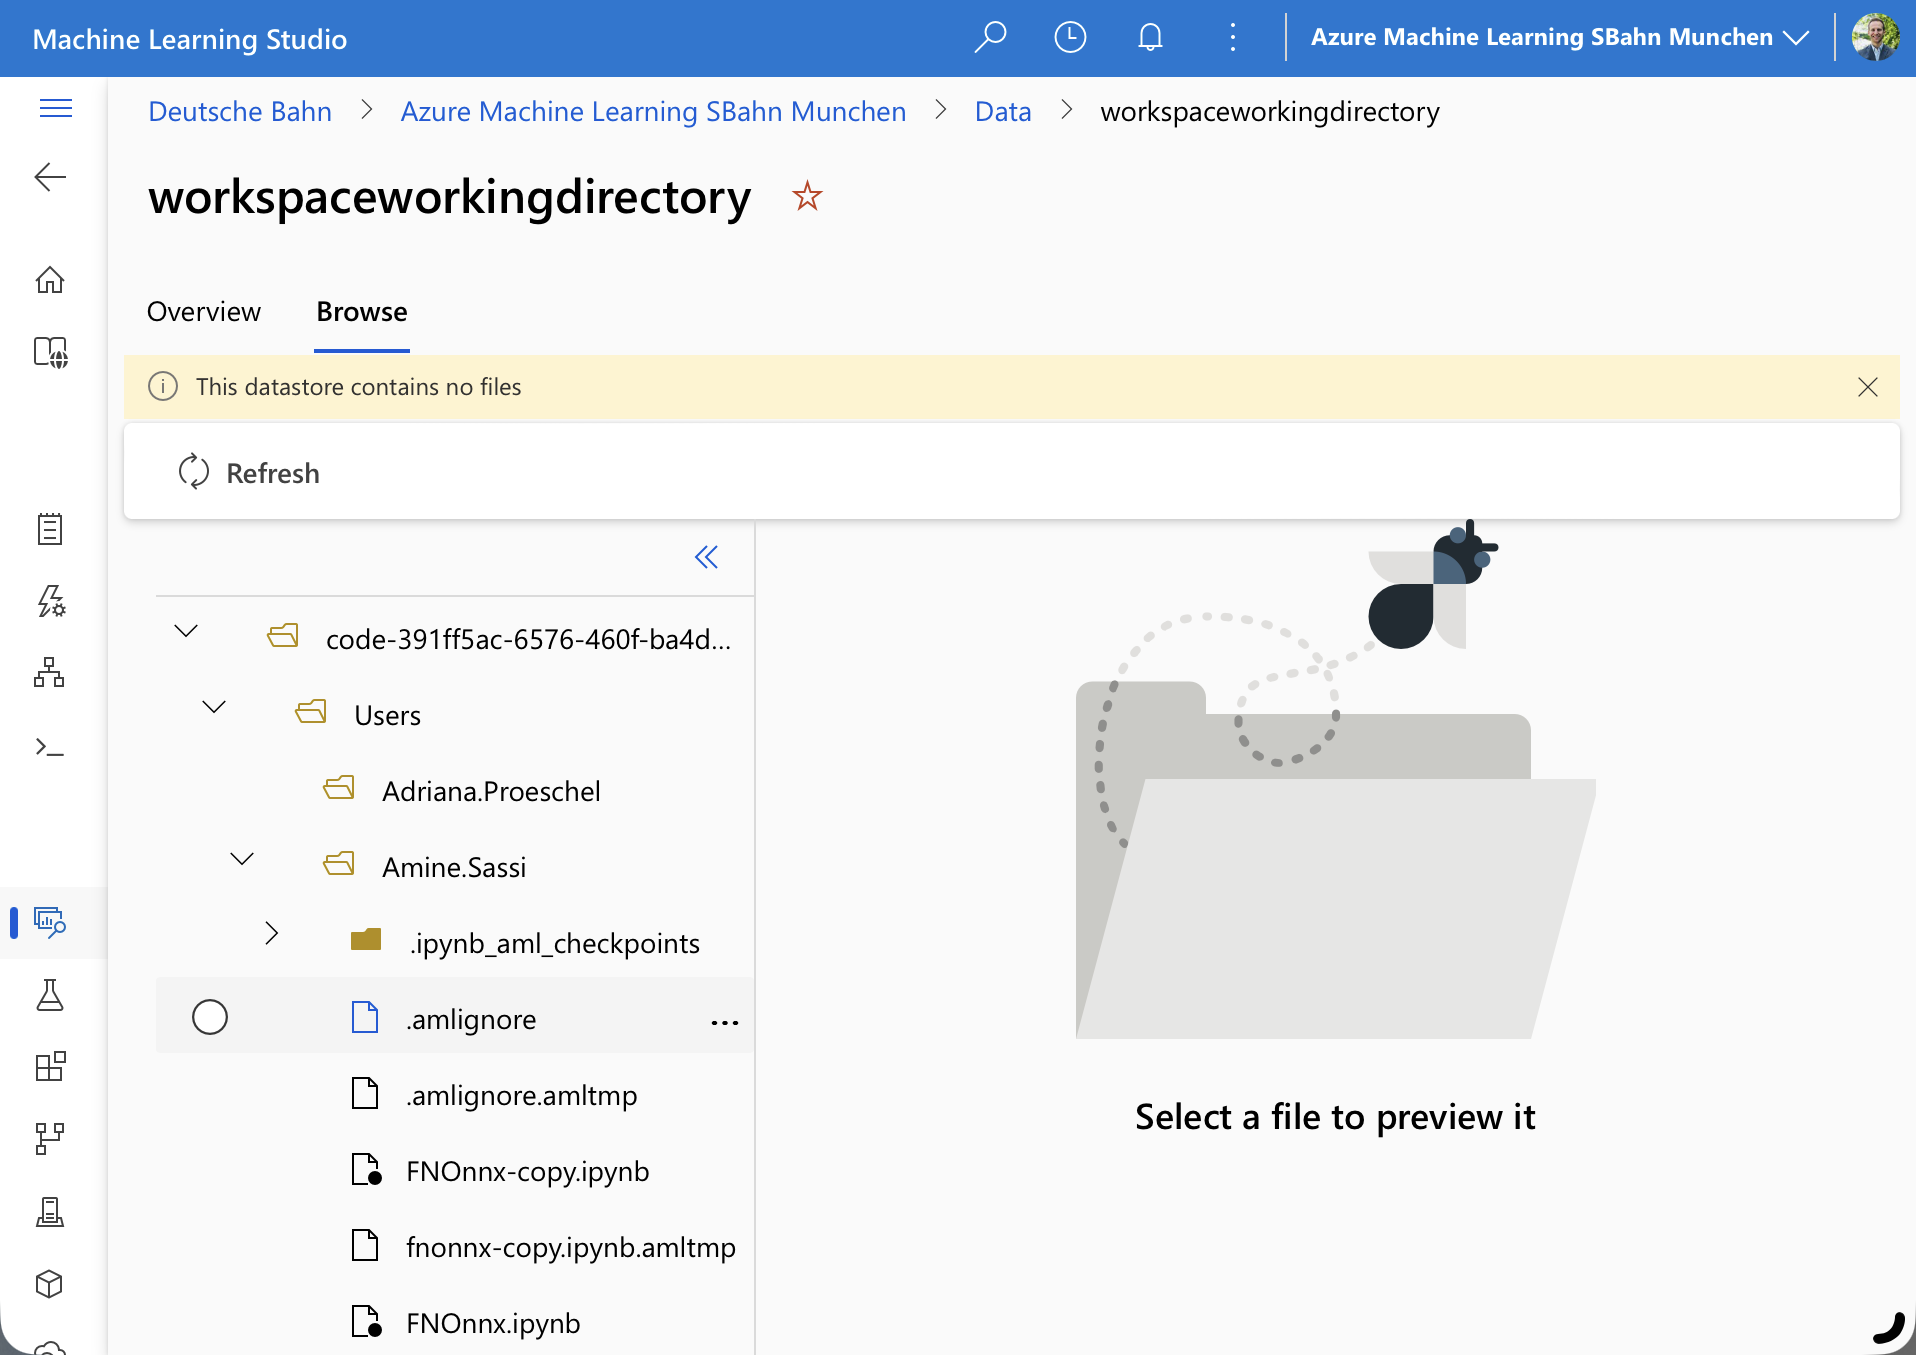
\includegraphics[scale = 0.1]{attachment/chapter_10/Scc038}
		\caption{Model/ Other own created scripts/ notebooks}
	\end{figure}
	\item[Notebook Files] as been shown, in the workspaceworking dircotry are more then just the notebook files. 
		\begin{figure}[H]
		\centering
		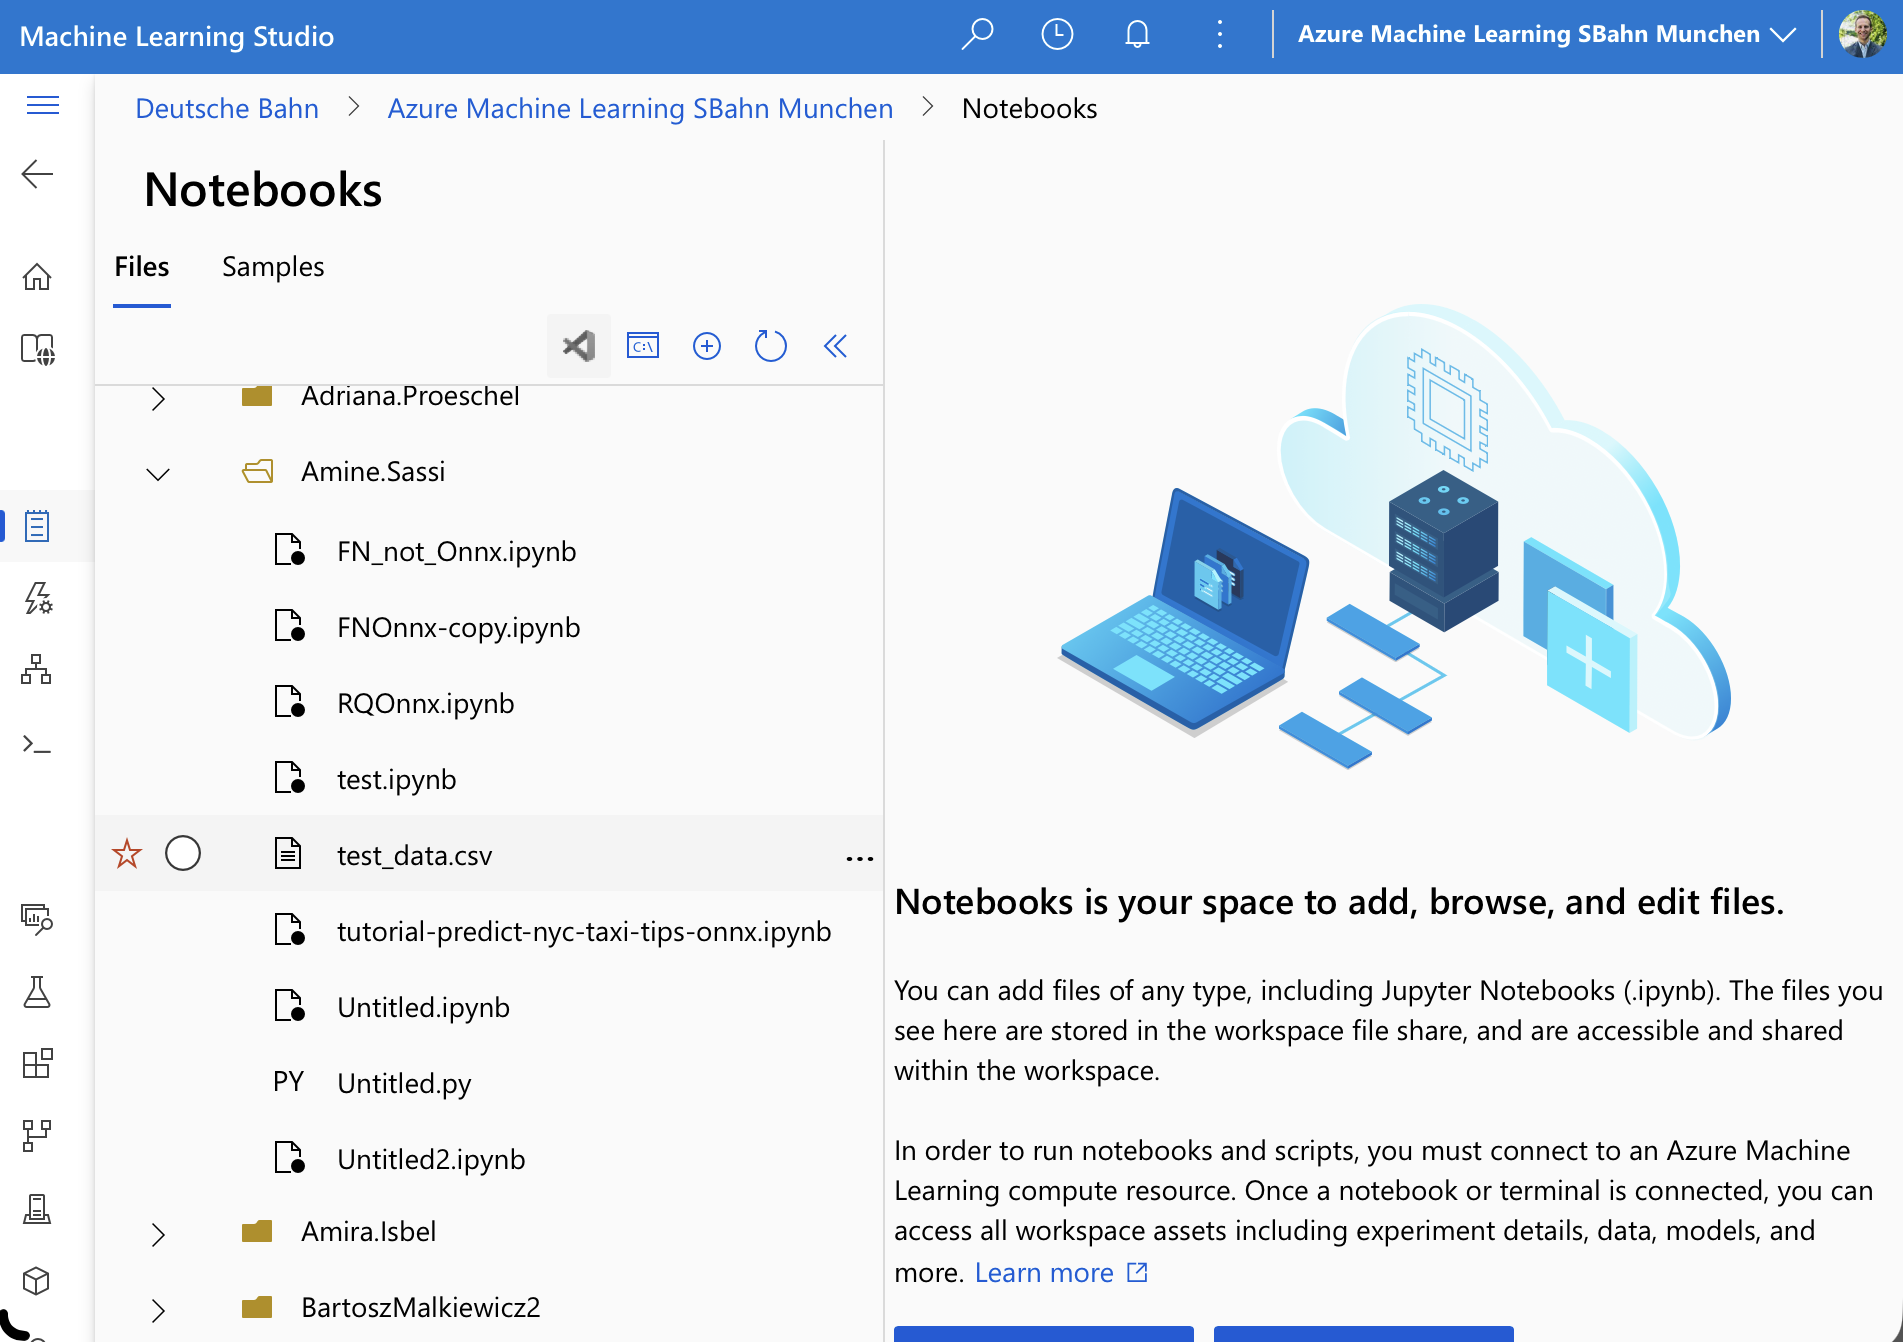
\includegraphics[scale = 0.1]{attachment/chapter_10/Scc039}
		\caption{Just Notebooks}
	\end{figure}
\end{description}

\subsubsection{Example: Blobstorage}

\begin{description}
	\item[workspaceblobstore (Default) (Store)] It looks like files, that are required to execute the pipeline or model.
	\begin{figure}[H]
		\centering
		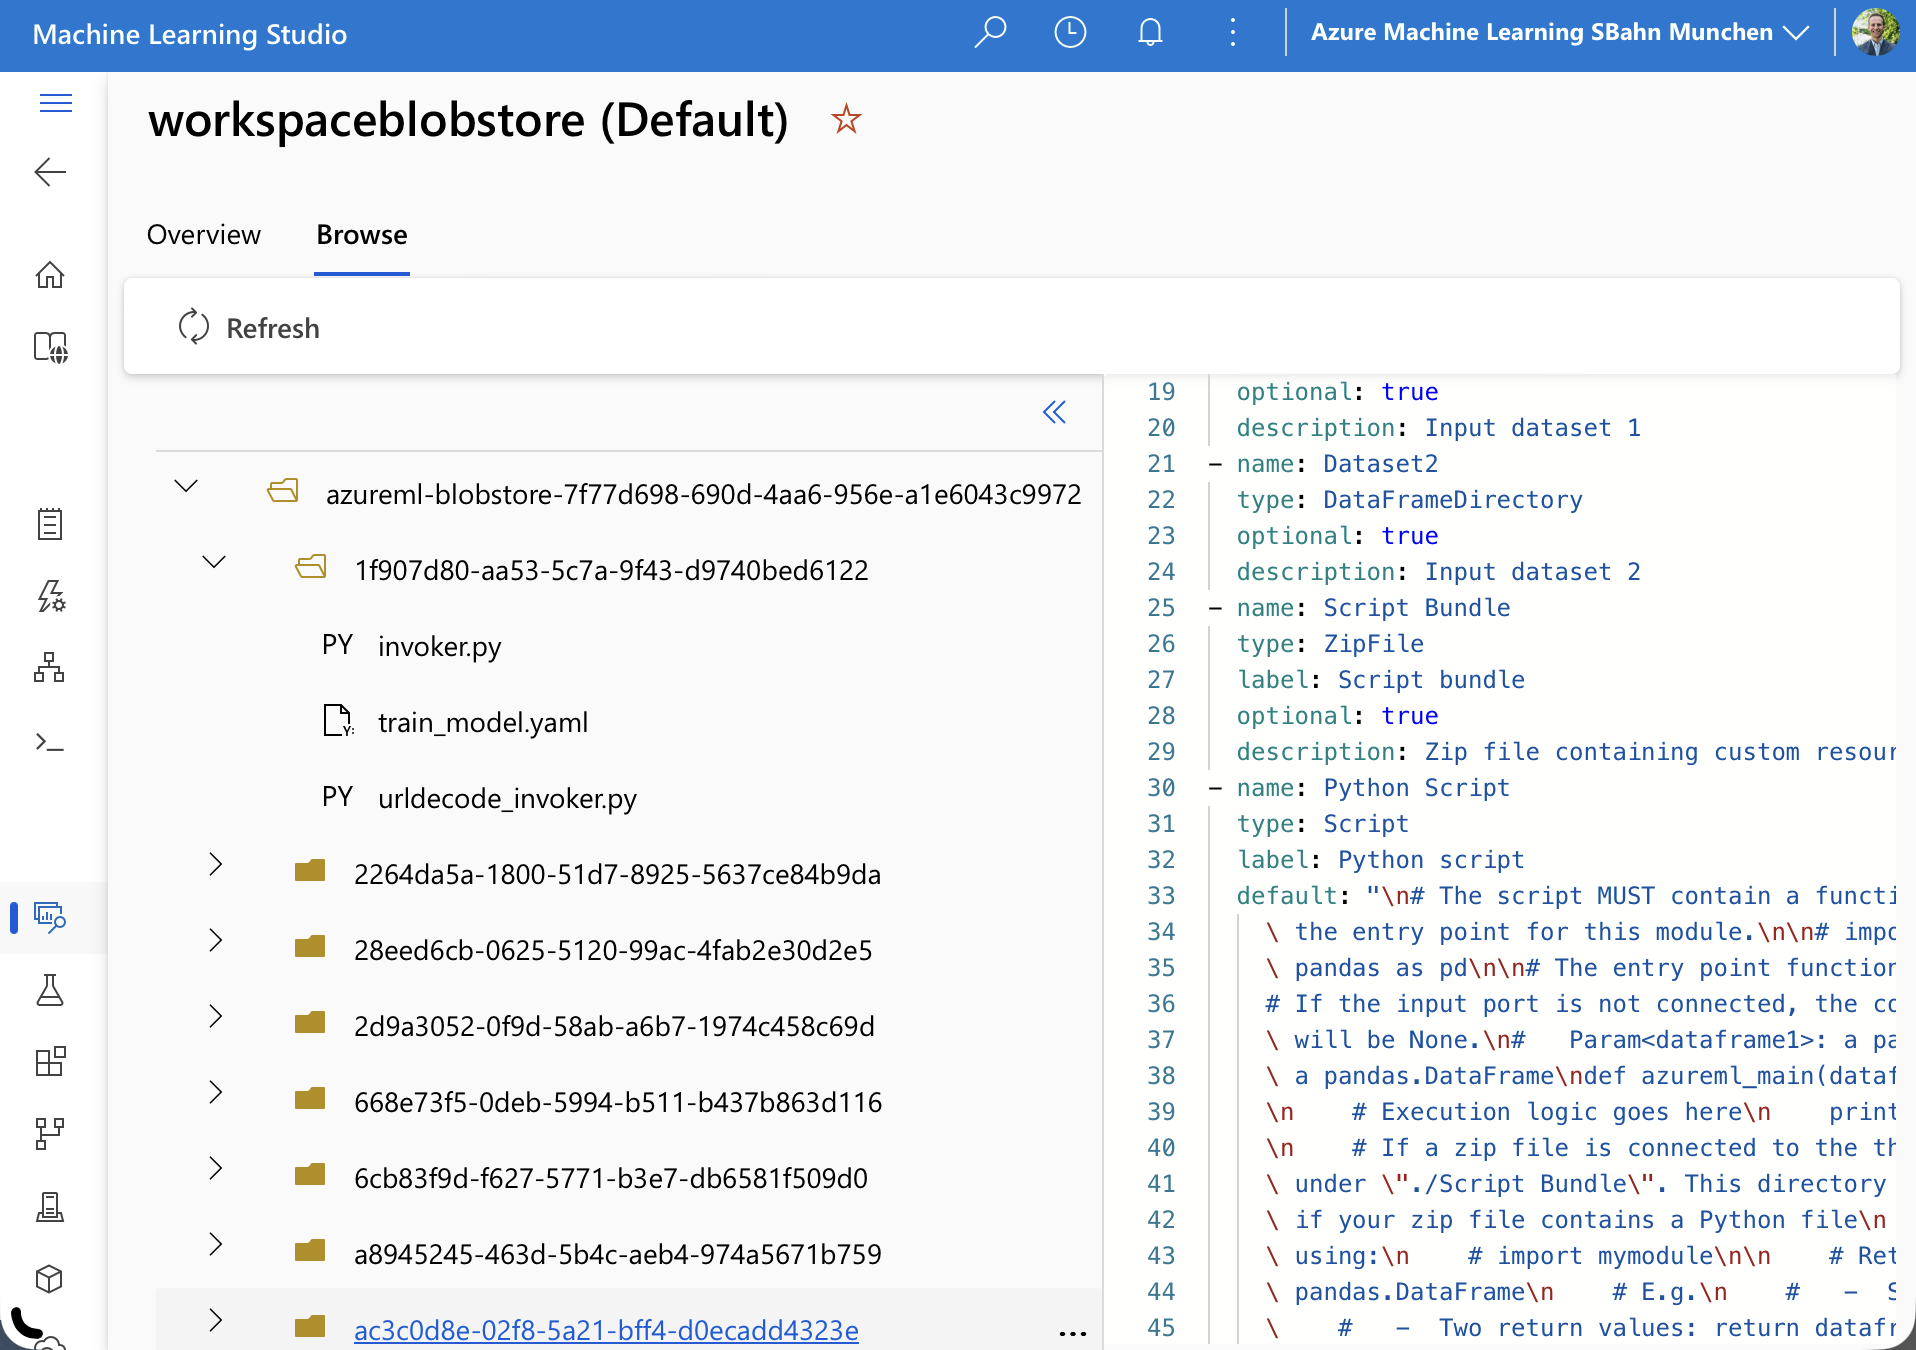
\includegraphics[scale = 0.3]{attachment/chapter_10/Scc041}
		\caption{Bit unclear, what does files are.}
	\end{figure}
	\item[worksapceartifactstore (Store)] It tracks logs for the experiment runs, compute runs and so on.
		\begin{figure}[H]
		\centering
		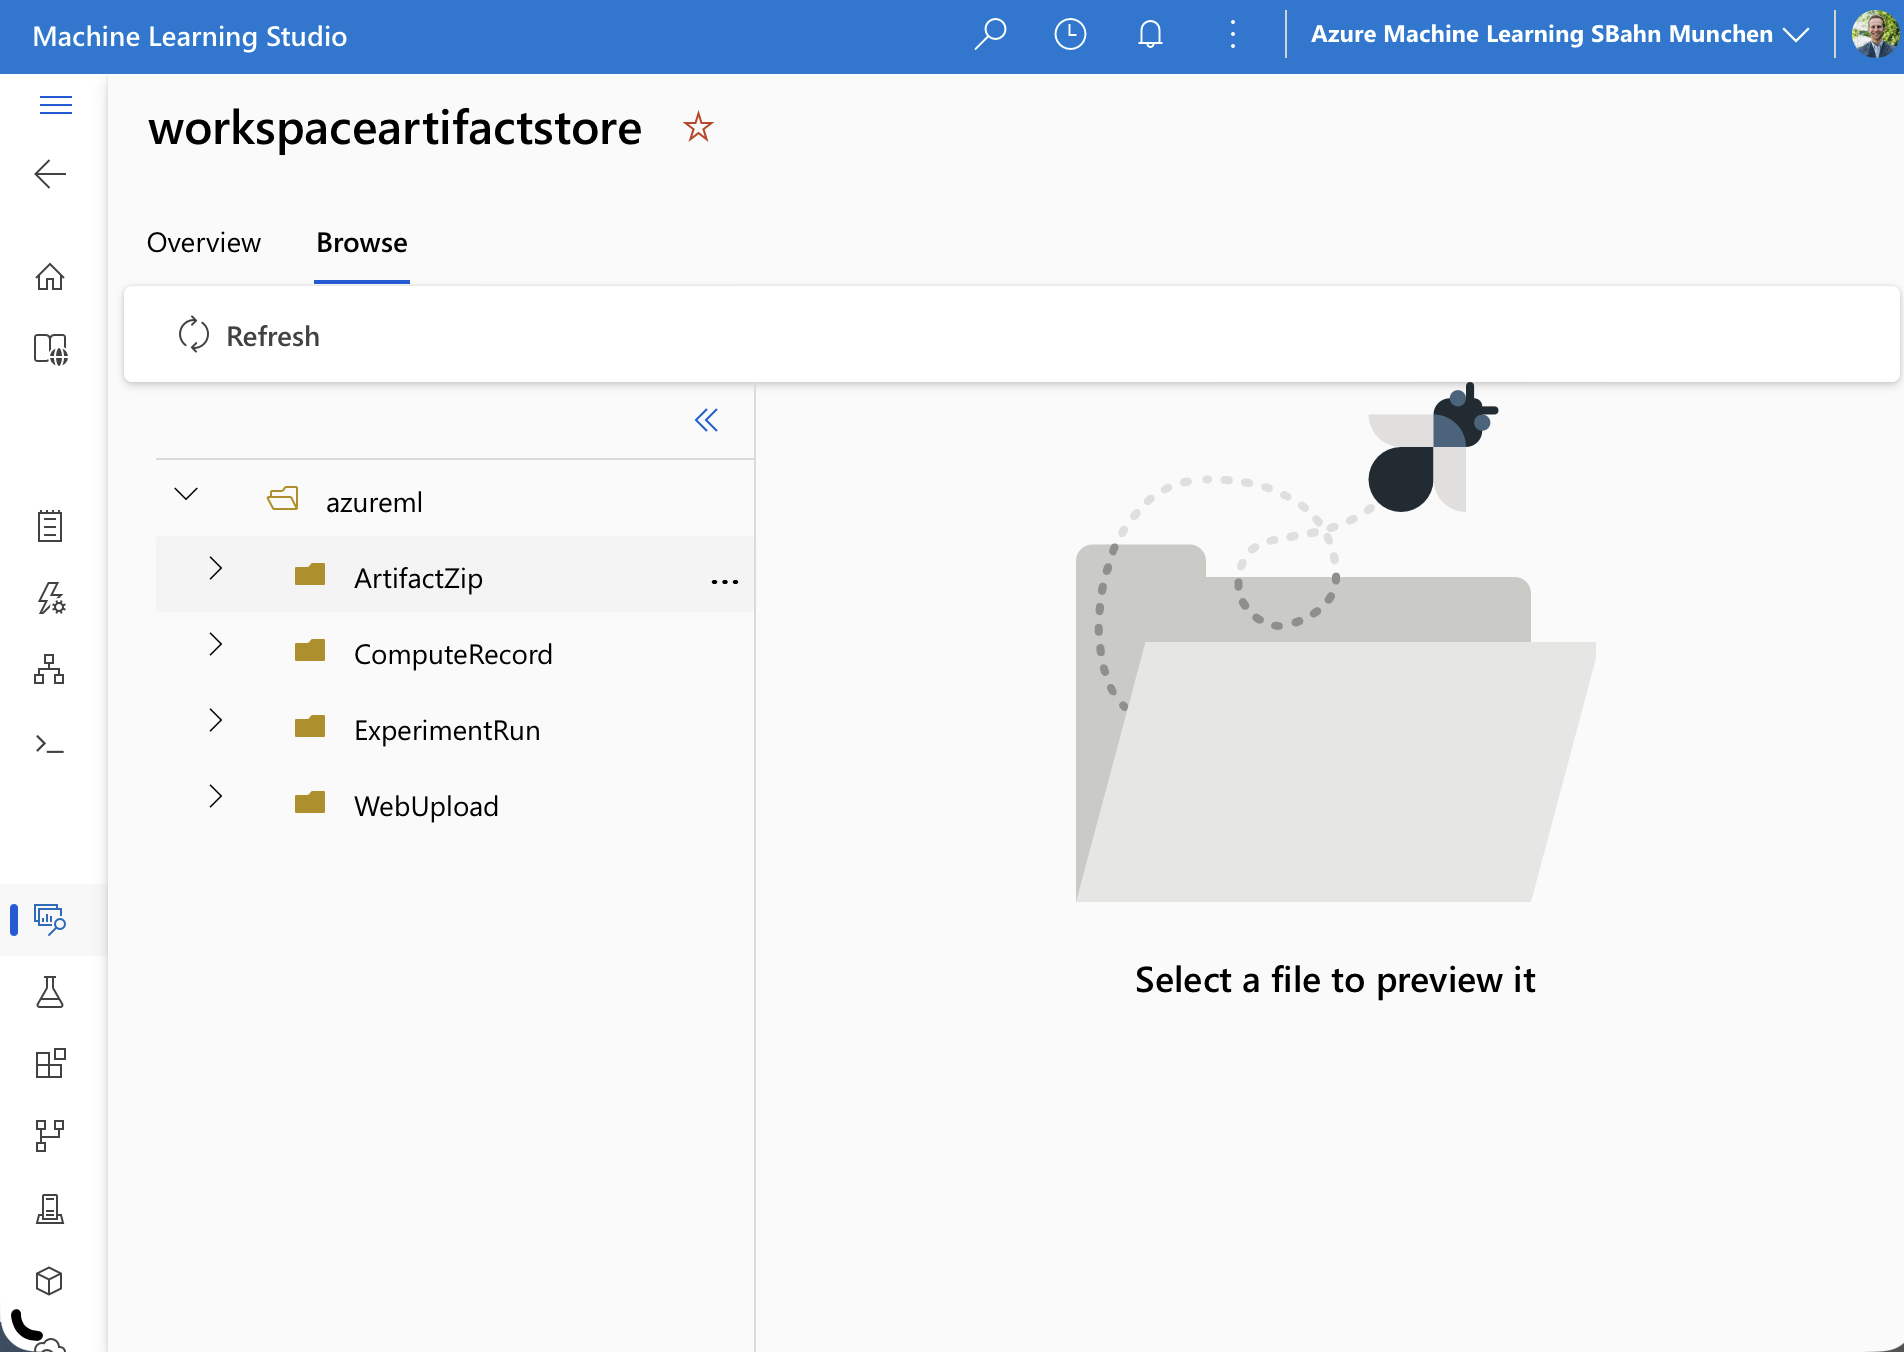
\includegraphics[scale = 0.3]{attachment/chapter_10/Scc040}
		\caption{Logging of al sorts of things}
	\end{figure}
\end{description}

\subsection{Compute Ressources}
The compute ressources which are needed for a explore data analysis, training or inferenceing can be managed directly in Azure ML. For this a \gls{VM} is spindup.\\

\begin{figure}[H]
	\centering
	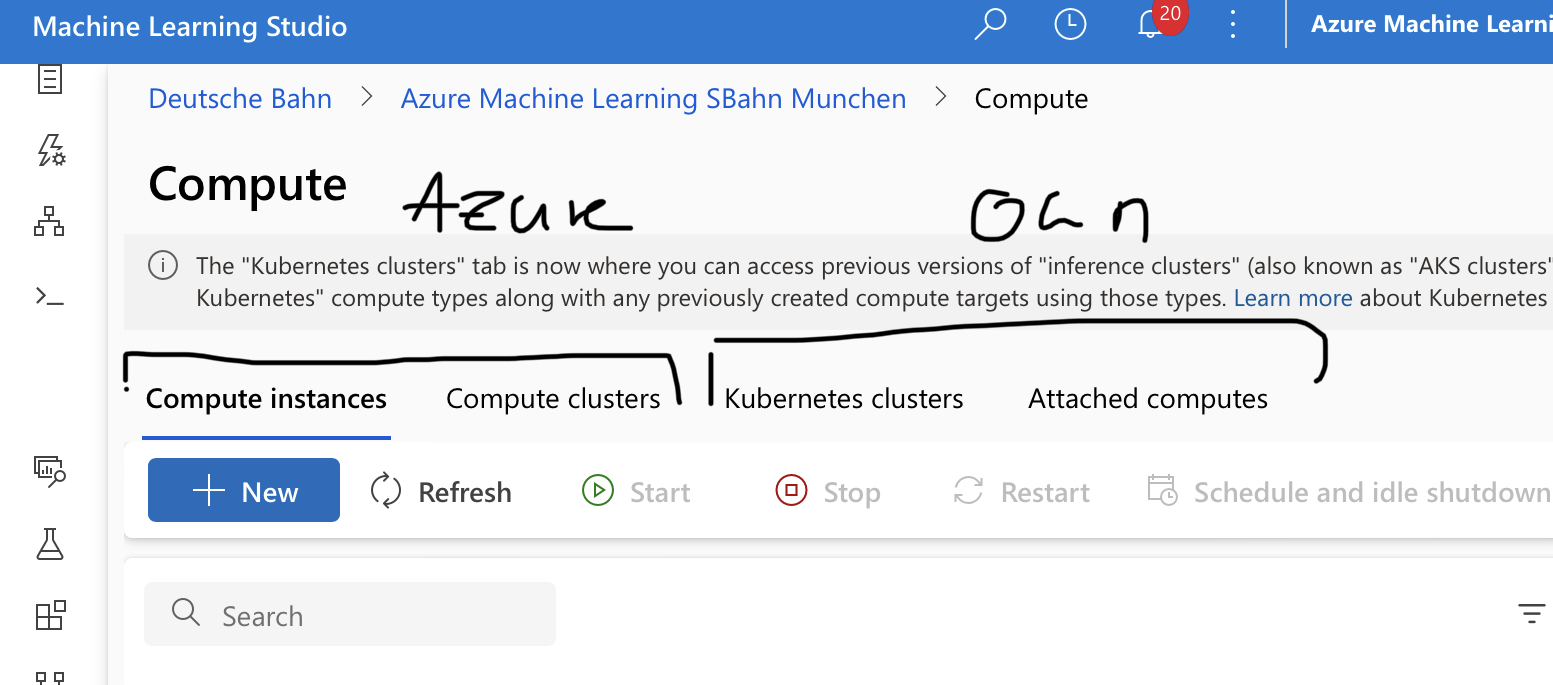
\includegraphics[scale = 0.1]{attachment/chapter_10/Scc030}\\ 
	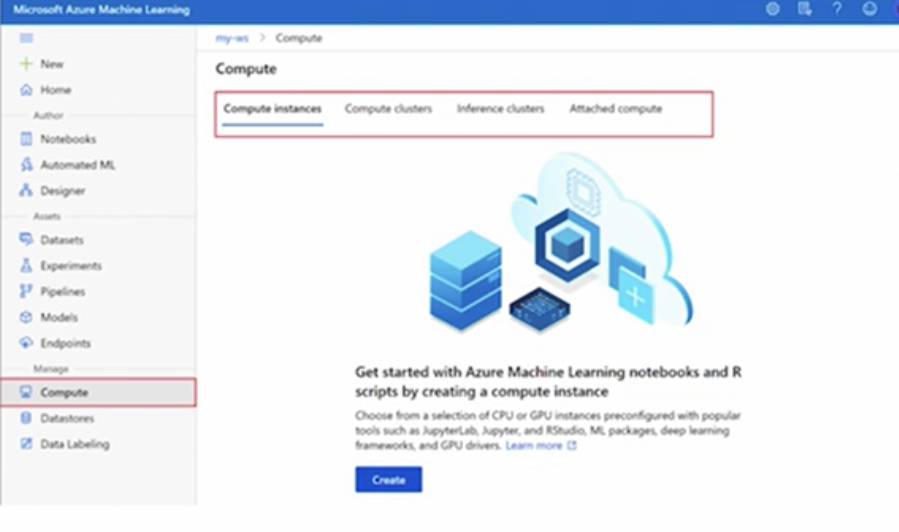
\includegraphics[scale = 0.1]{attachment/chapter_10/Scc031}
	\caption{Compute Types}
\end{figure}

\begin{itemize}
	\item The \textit{compute instance}/ \textit{compute cluster} is on or multiple \gls{VM}   for research and training the model.
	\item Also can be attached own \gls{VM}. 
	\item The field \textit{inference cluster} or new \textit{Kubernets cluster} allows to bring own cluster for the deployment process.
\end{itemize}


\textit{Note} For deployment with managed endpoints the this is spin up by it self.

\subsection{Model}
\subsubsection{Difference between ML and traditional Software}
In the traditional programming a problem is adressed, by having input data and designing a programm, which transforms this data to a desired output. The logic is hard coded.\\ 

With \gls{ML} a $"$Model$"$ derives the logic form the input and combined output data. This logic can be updated - trained over time. The model is the \textit{anwser} to the problem. Most of the time, it is unclear, why, but the evaluation of the model takes care of this.

\begin{figure}[H]
	\centering
	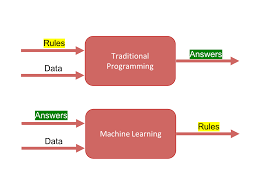
\includegraphics[scale = 0.1]{attachment/chapter_10/Scc034.PNG}
	\caption{Output is a Model}
\end{figure}

The learned model is trained on input and output data. This is then deployed as the $"$traditional$"$ programm.

\begin{figure}[H]
	\centering
	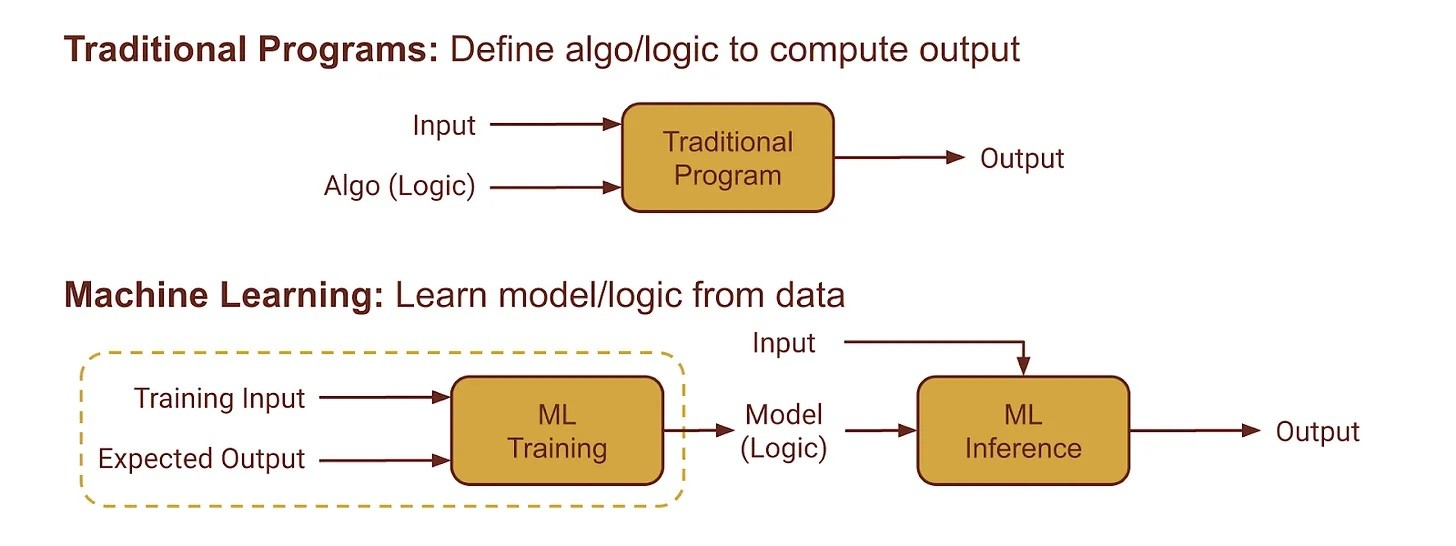
\includegraphics[scale = 0.1]{attachment/chapter_10/Scc035.JPG}
	\caption{Deployment of the Model}
\end{figure}

\subsection{Pipelines Designer}
\subsubsection{Example: Simple Model}
A no-code option is \textit{Designer}. It allows for a click-drop design of the process. From 
\begin{itemize}
	\item data ingestion,
	\item training,
	\item scoring
	\item to validating
\end{itemize}
the process steps can be selected by linked modules.

\begin{figure}[H]
	\centering
	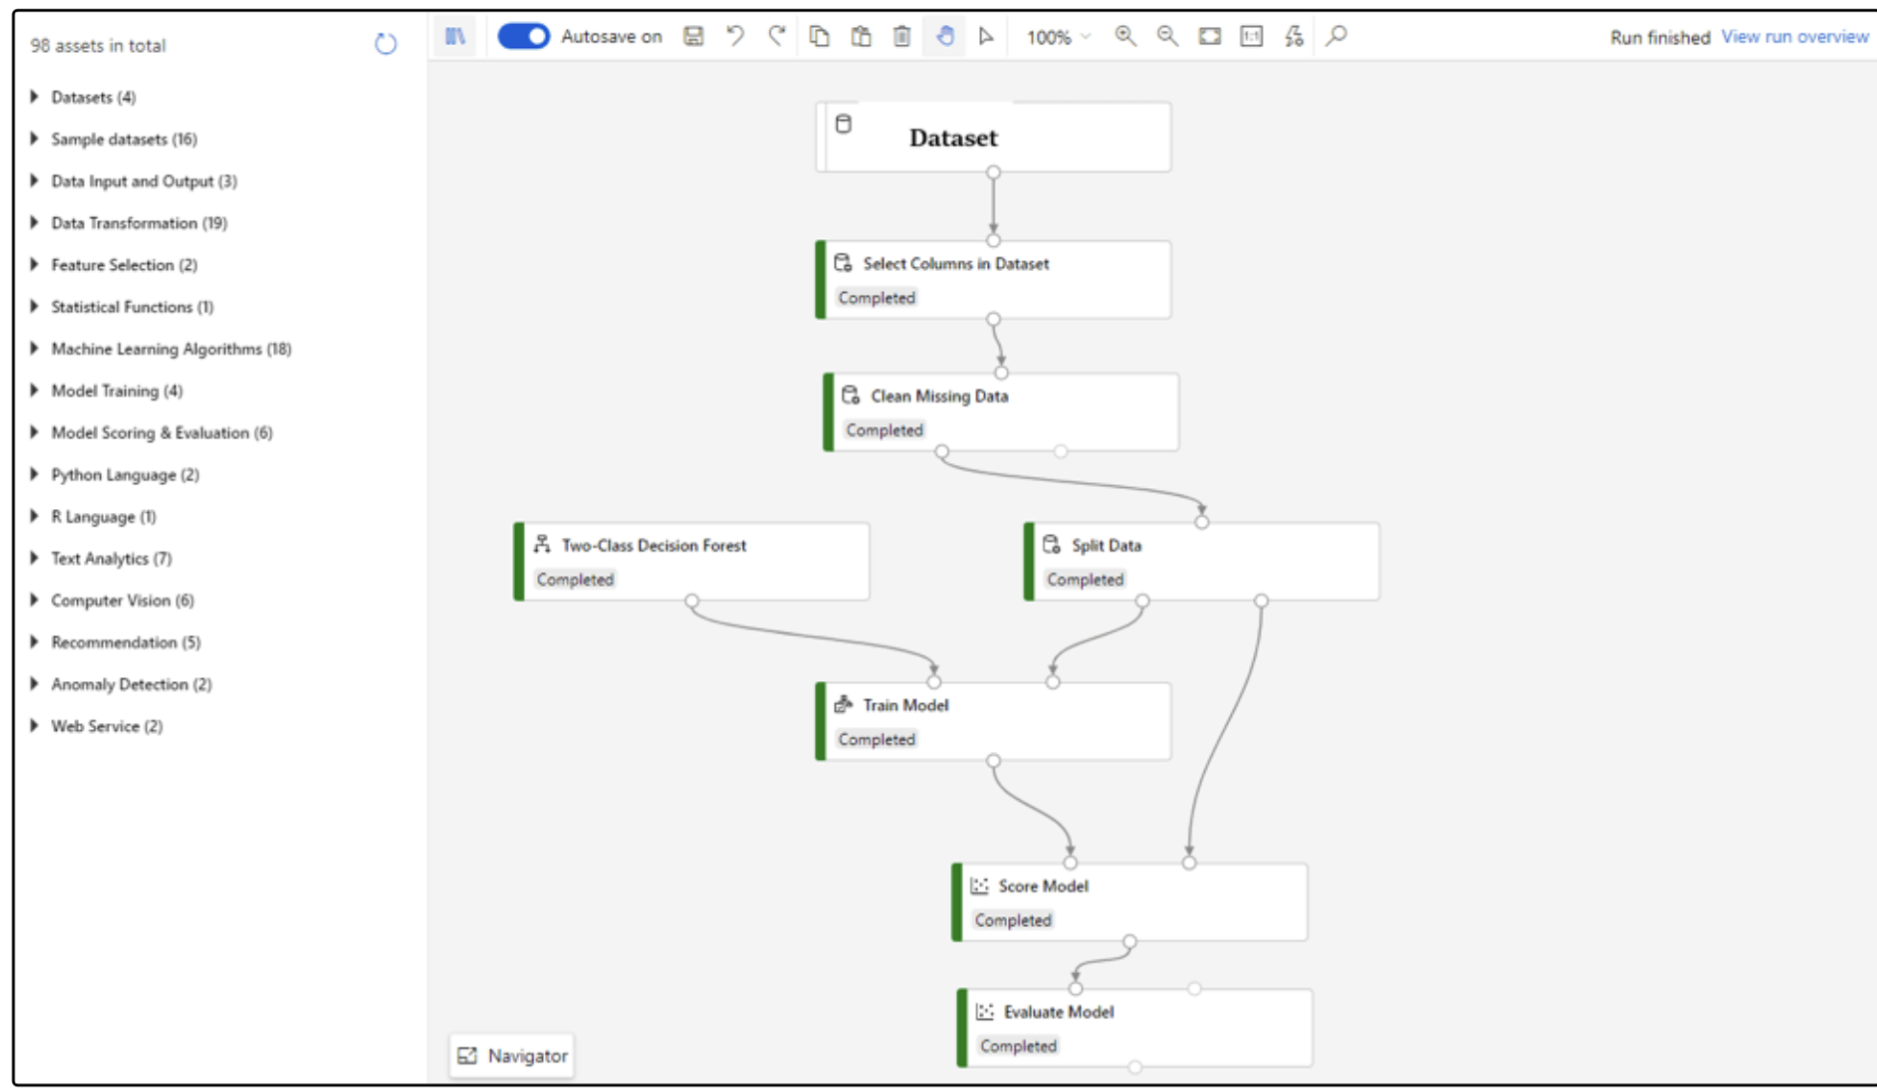
\includegraphics[scale = 0.3]{attachment/chapter_10/Scc005}
	\caption{Example Process}
\end{figure}

In this simple example a model will be a part of the pipeline. The steps in a \gls{ML} process are finding the right feature, cleaning the data, then spliting the data, train a model with a algorithm as a input and then score the rest of the dataset (splited), which was not used for training the model. The results of the scored data are then evaluated.


\subsection{Notebooks}
\subsubsection{git repo Integration} \label{subsub:git_repo}
It is possible to clone a repo into \textit{workspacefilestorage}. This is done over the terminal function.

\begin{figure}[H]
	\centering
	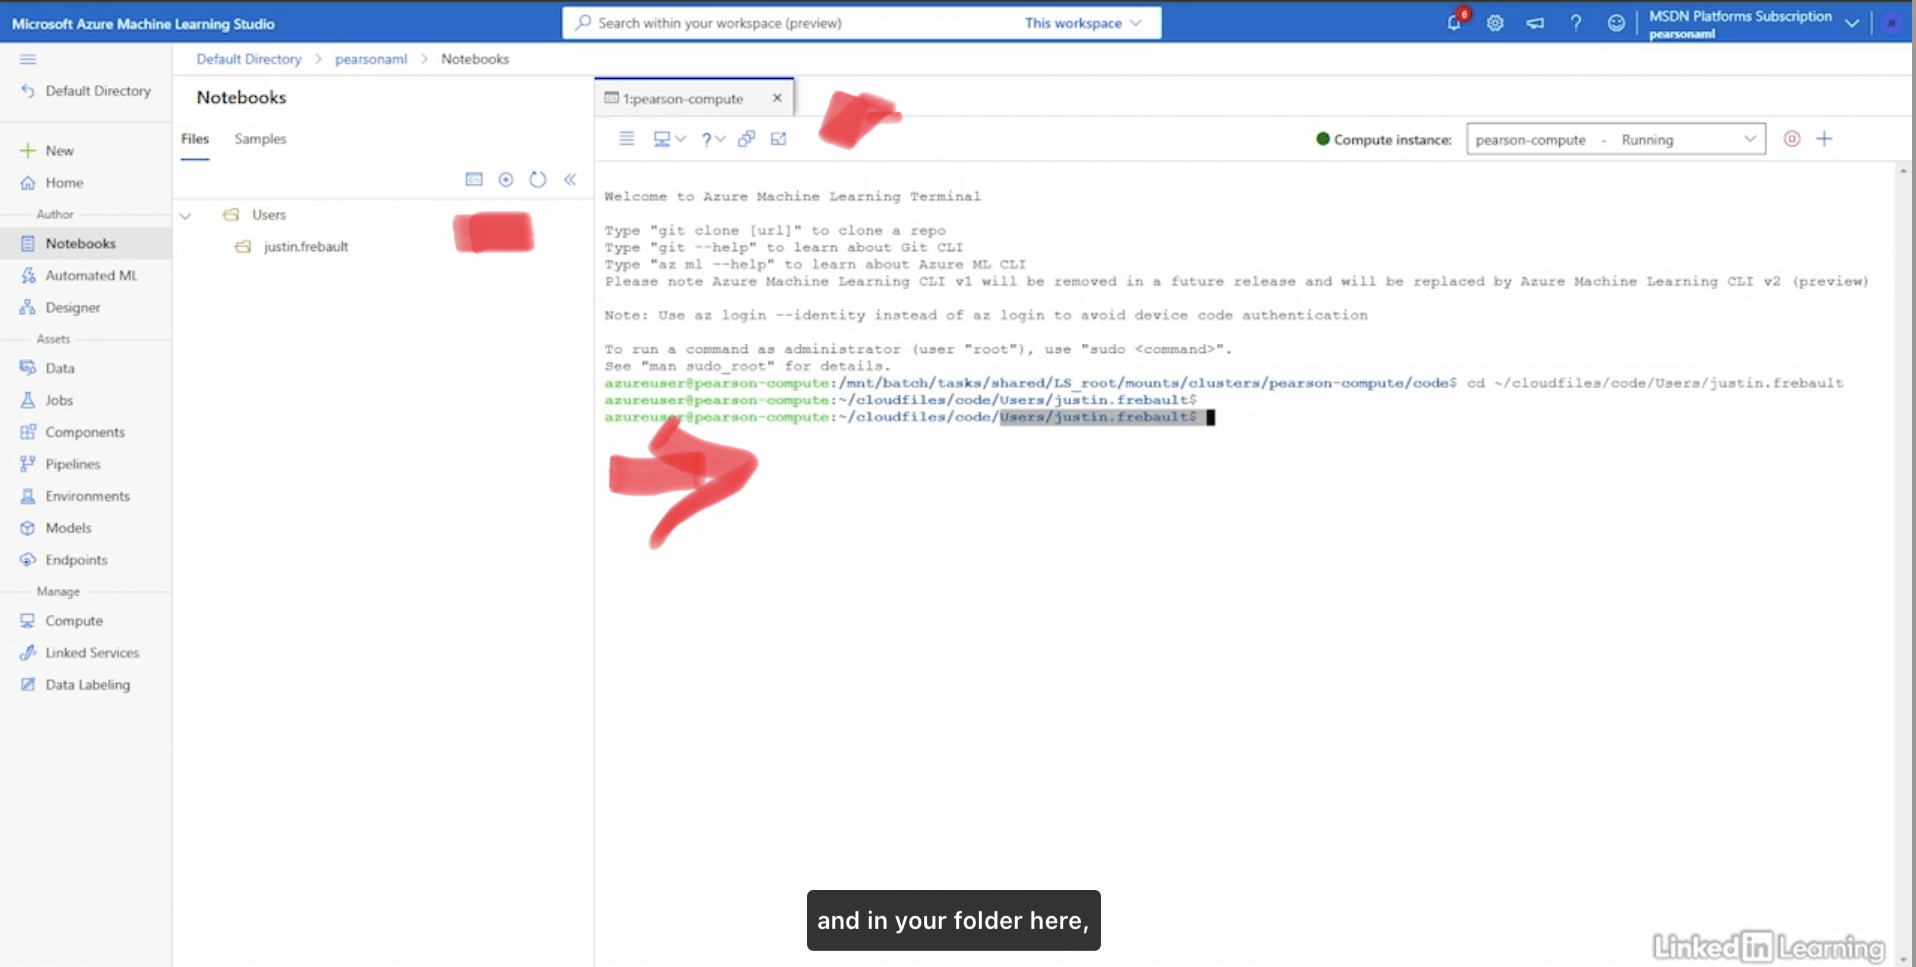
\includegraphics[scale = 0.2]{attachment/chapter_10/Scc042}
	\caption{Open Terminal}
\end{figure}

Provides with the url of the repo, this can be cloned into the filesystem. 
\begin{lstlisting}[style=CMD]
	git clone https://gitlab.com/justin.frebault/pearson-course-aml
\end{lstlisting}

\begin{figure}[H]
	\centering
	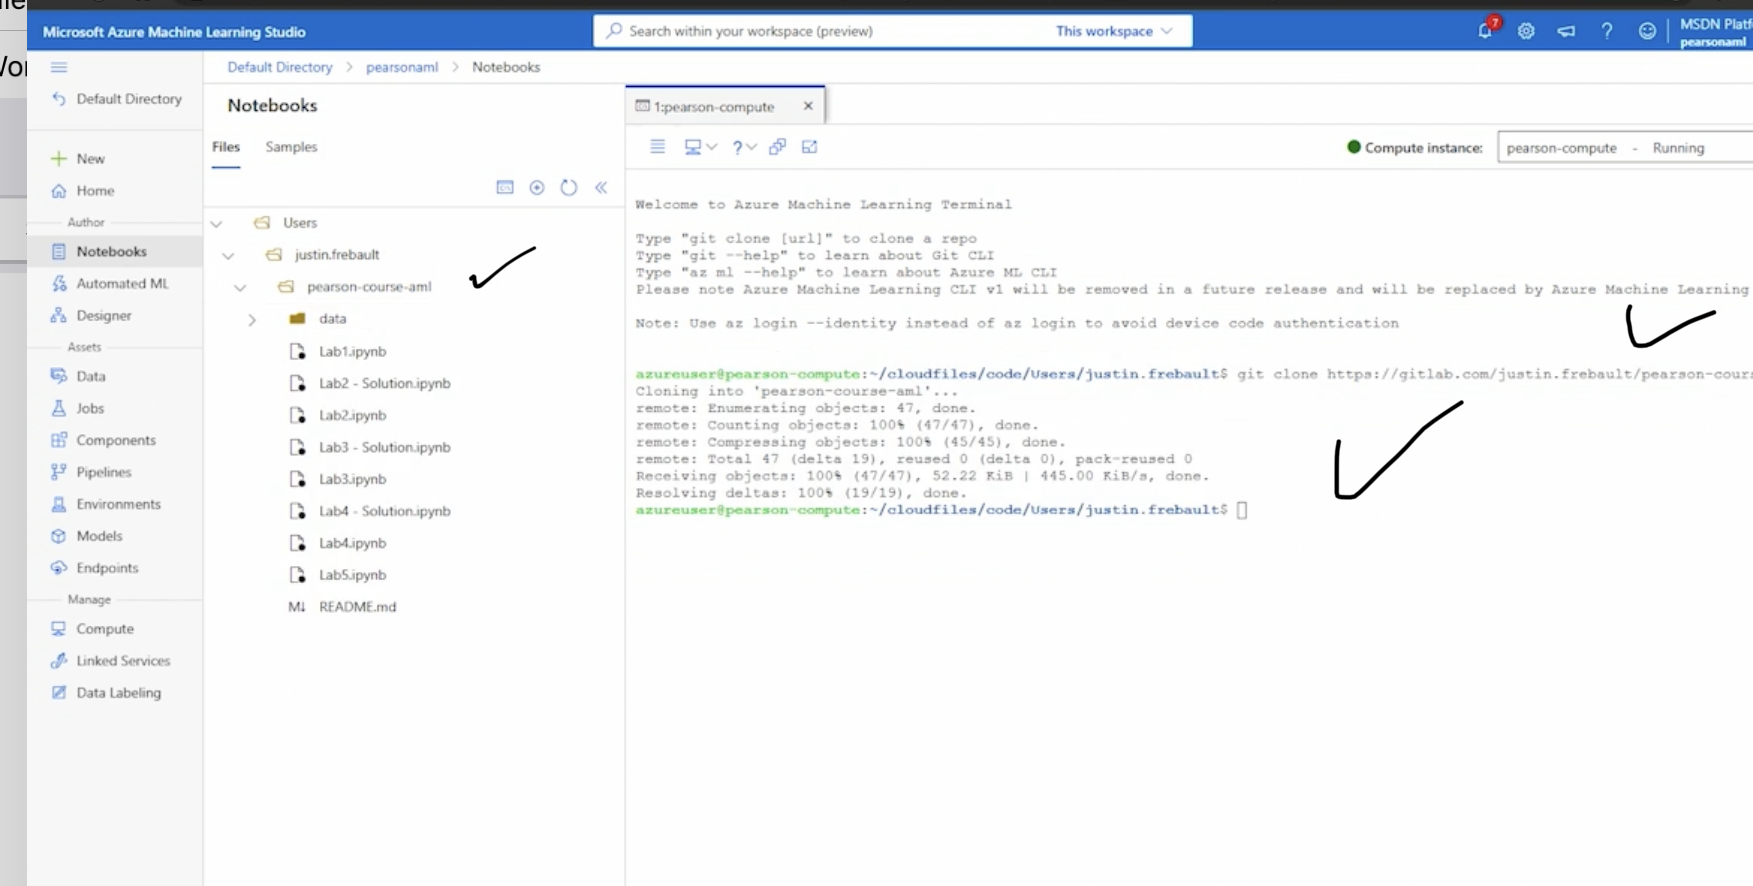
\includegraphics[scale = 0.3]{attachment/chapter_10/Scc043}
	\caption{Clone Repo}
\end{figure}

\textit{Note:} The file is only for testing. The filestorage account is not for storing data. In the workspacefile storage account is the full view of all the files for the cloned repo.

\begin{figure}[H]
	\centering
	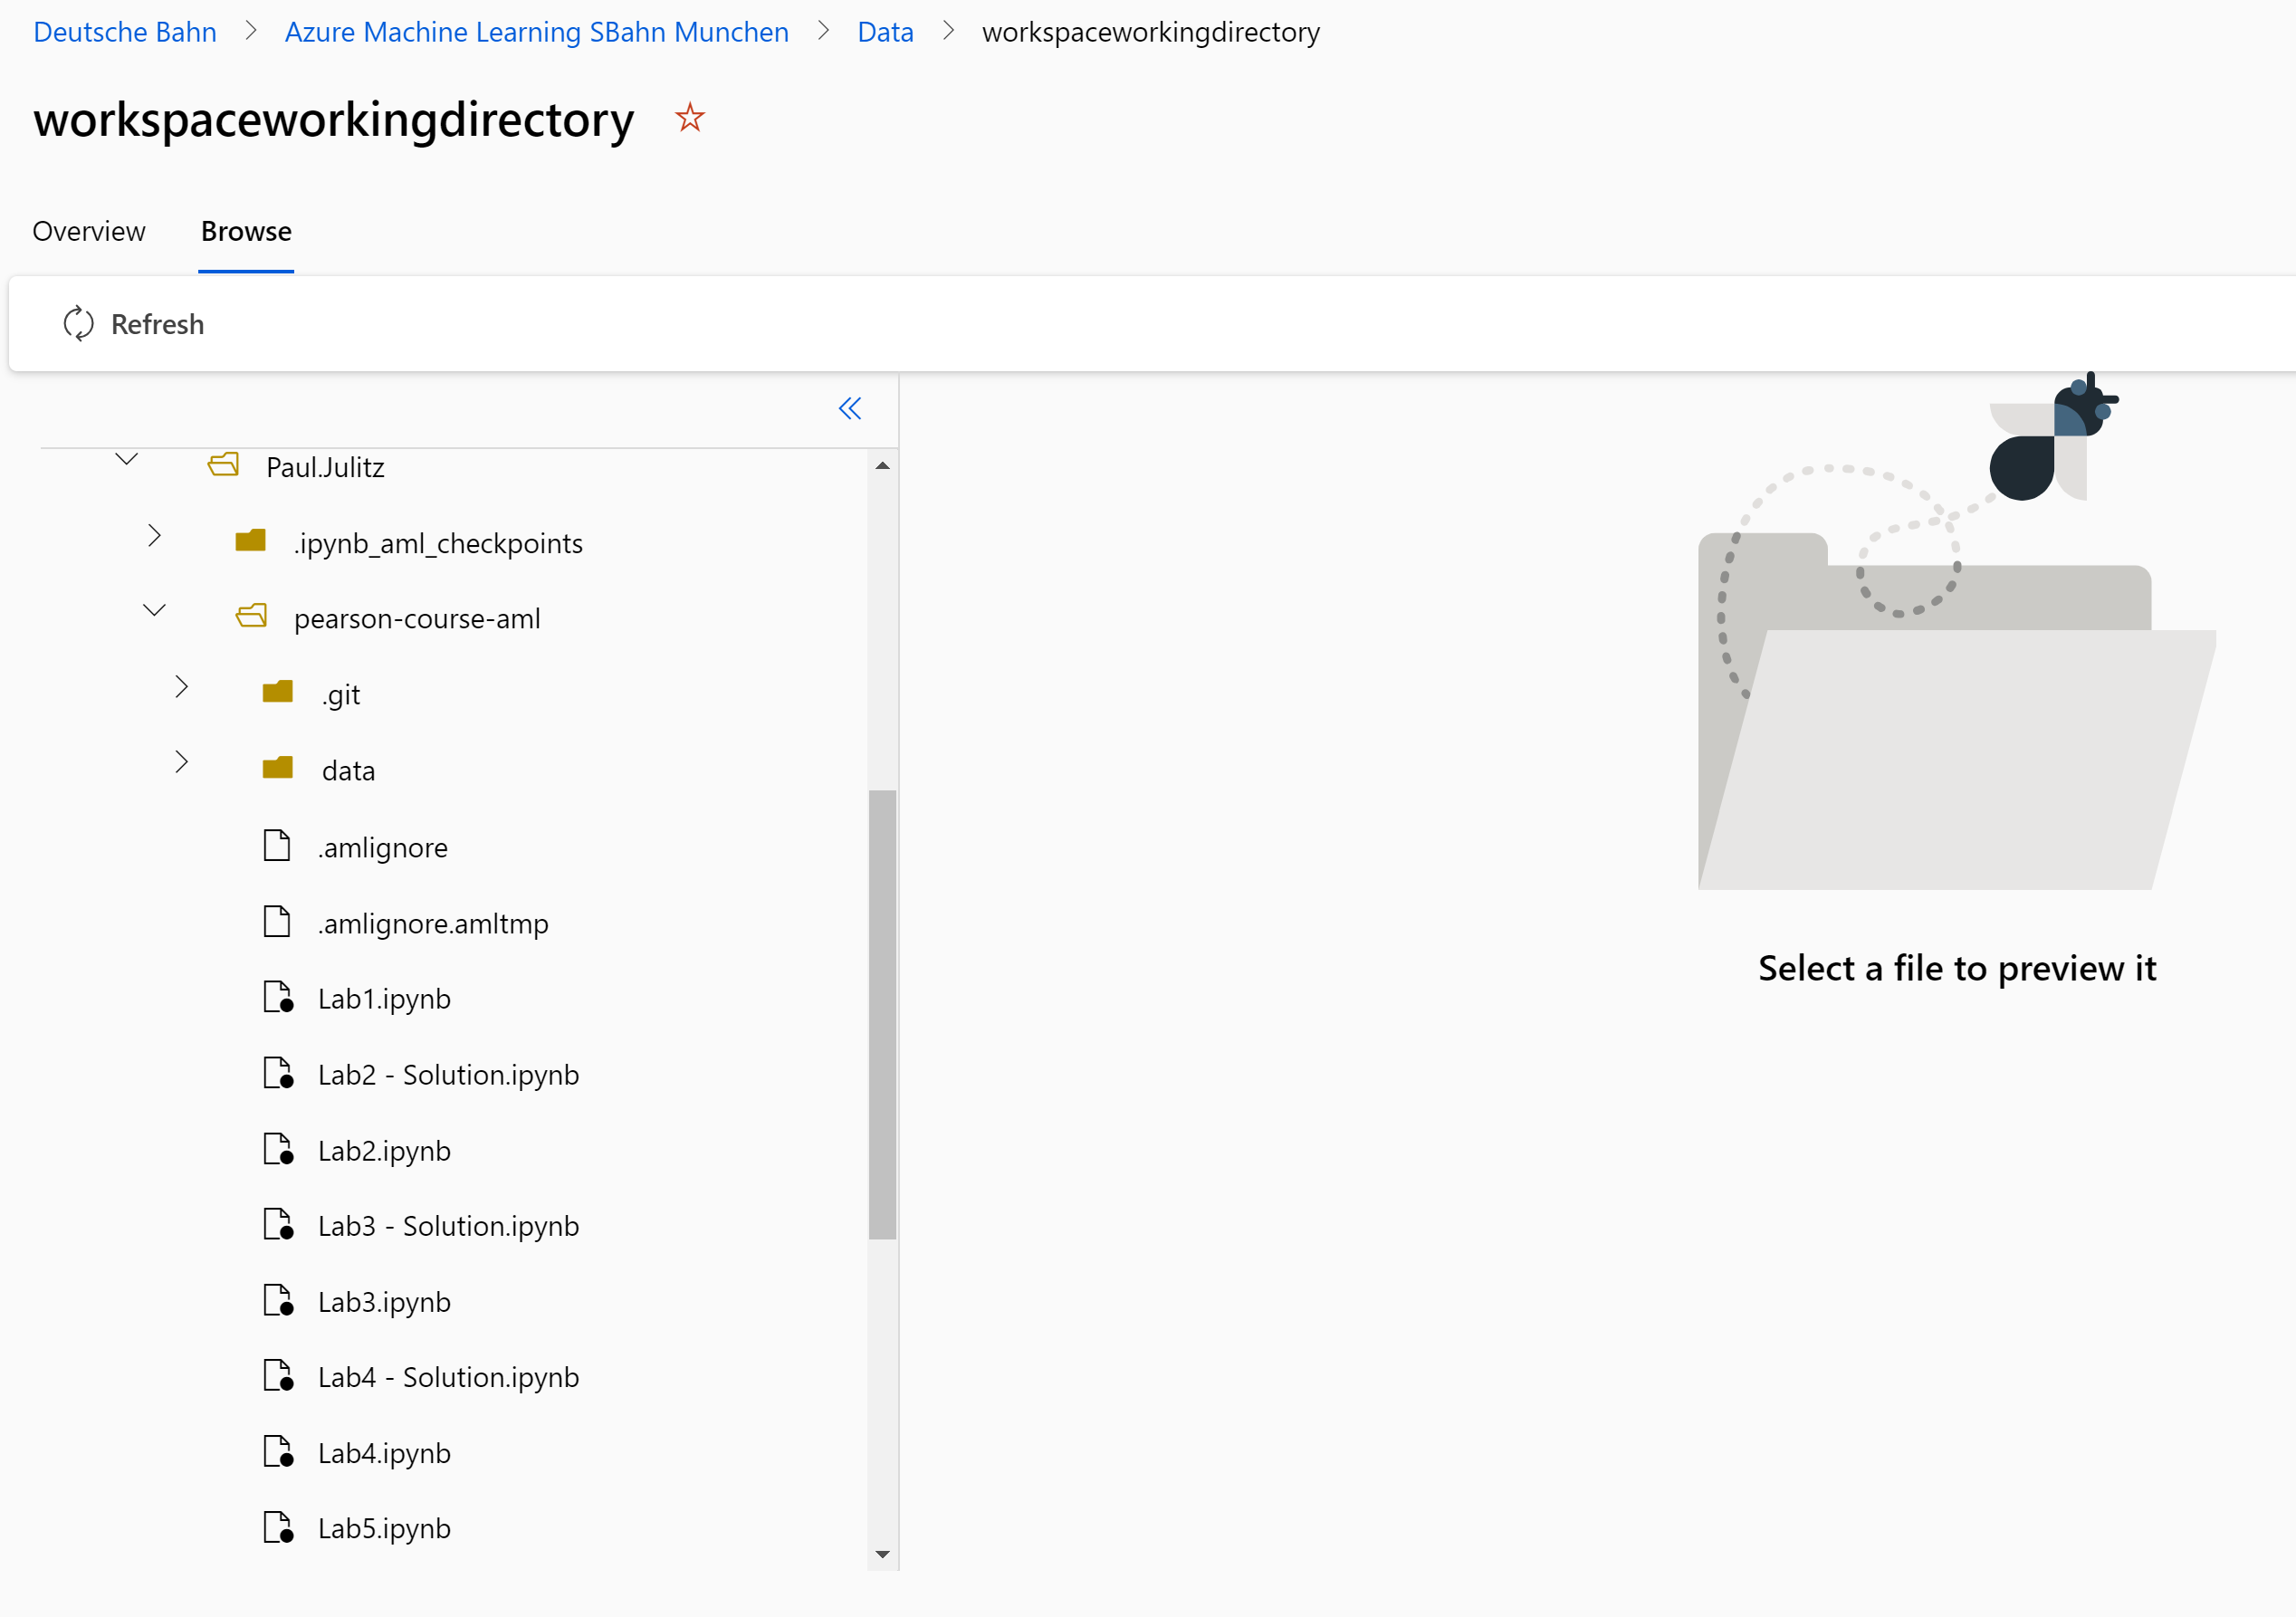
\includegraphics[scale = 0.3]{attachment/chapter_10/Scc045}
	\caption{View over data storage}
\end{figure}


\begin{figure}[H]
	\centering
	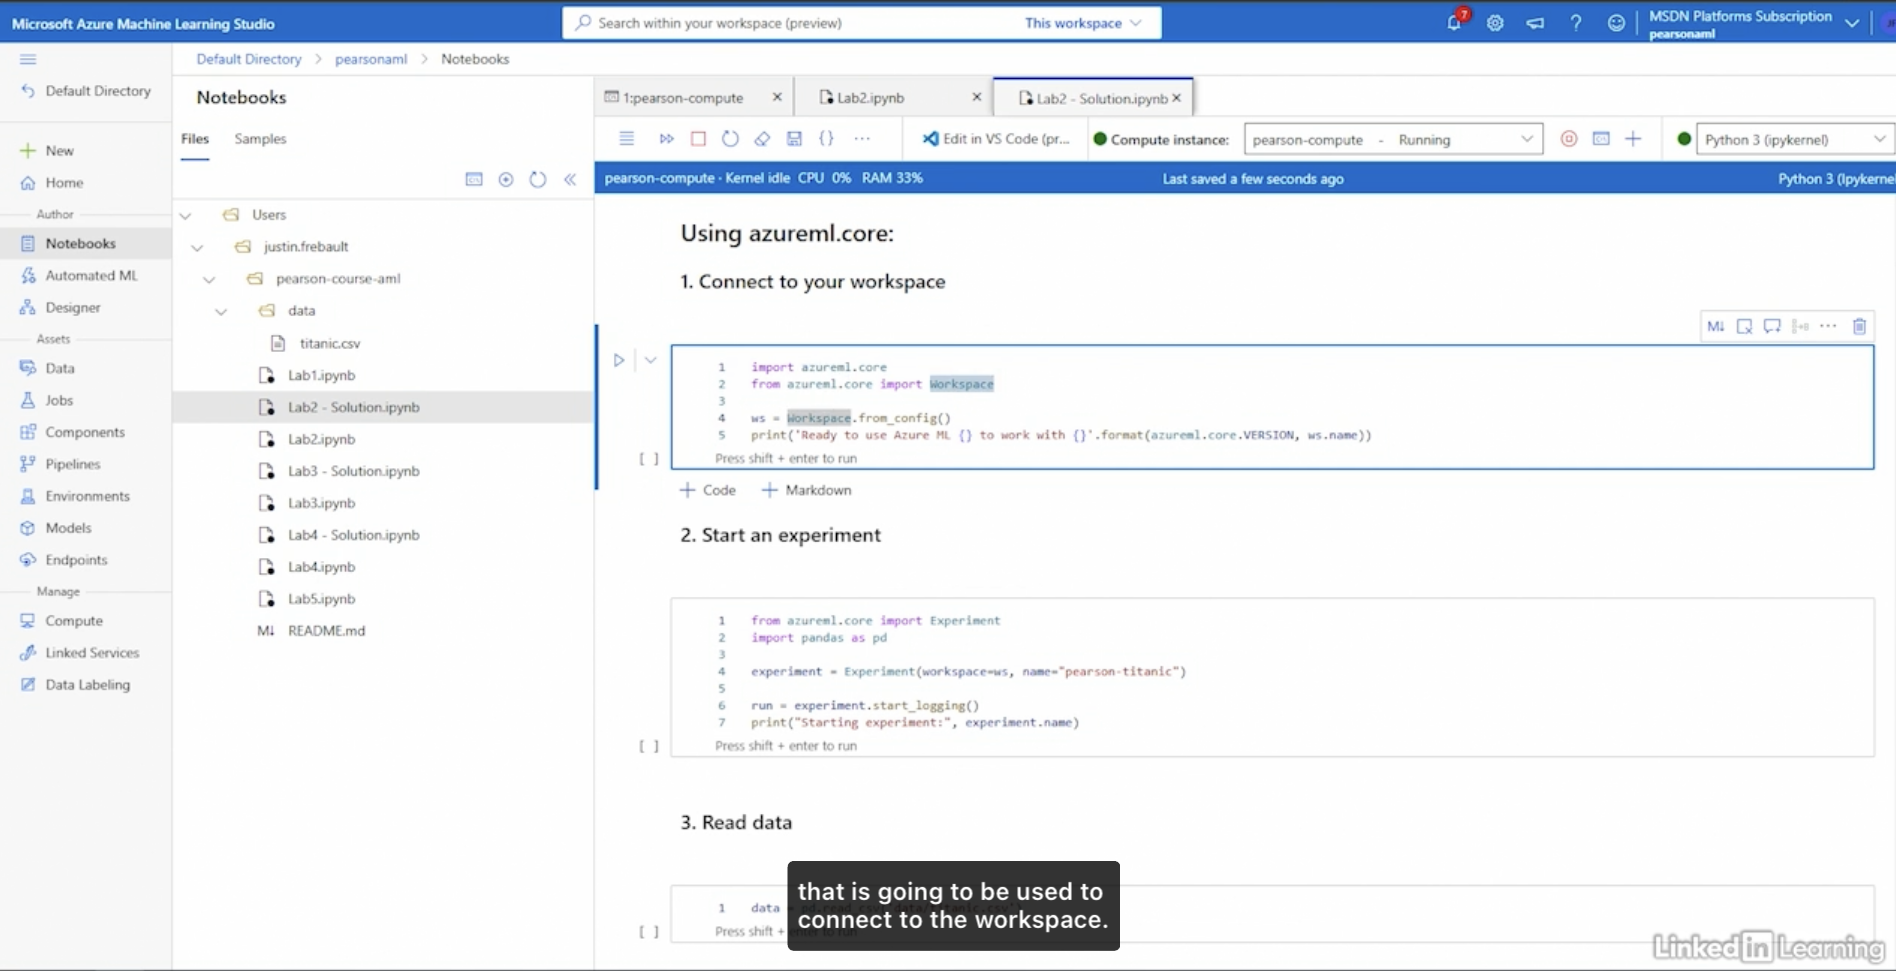
\includegraphics[scale = 0.3]{attachment/chapter_10/Scc044}
	\caption{Connecting to the data source}
\end{figure}

\subsubsection{Using VStudio Code}
The notebook can also be used and accessed with \textit{VStudio Code (Desktop)} or \textit{VStudio Code (Browser)}.

\begin{figure}[H]
	\centering
	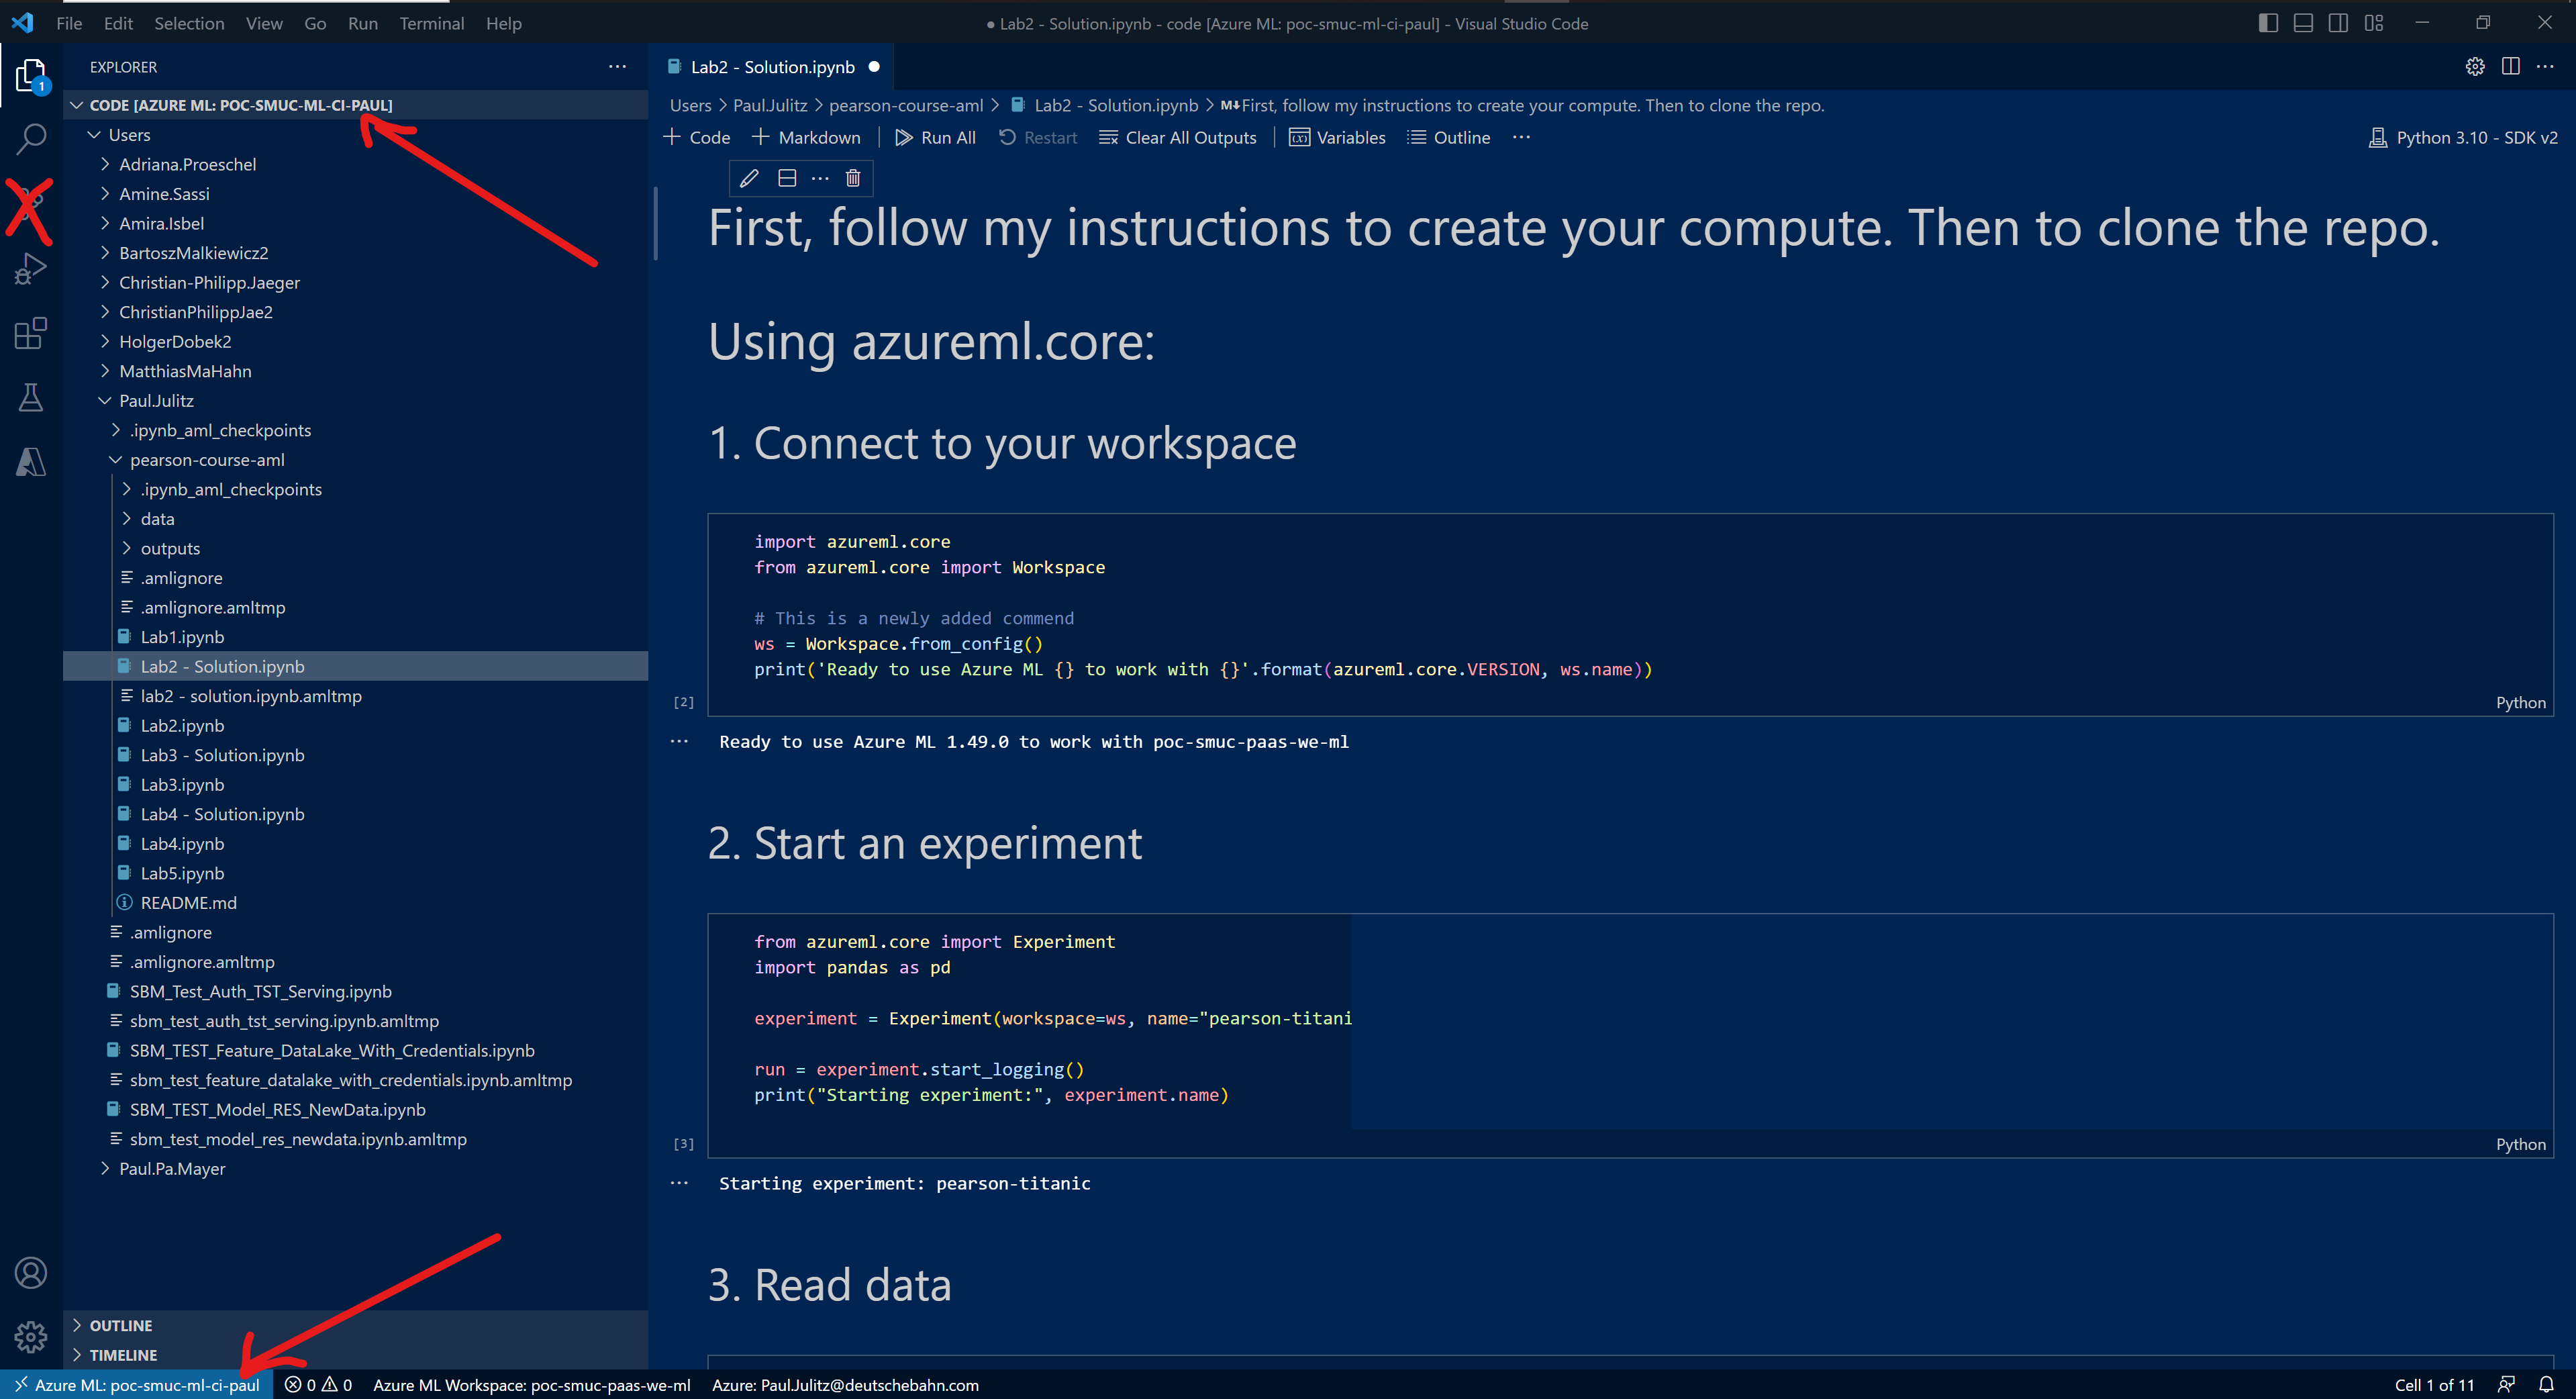
\includegraphics[scale = 0.1]{attachment/chapter_10/Scc048}\\
	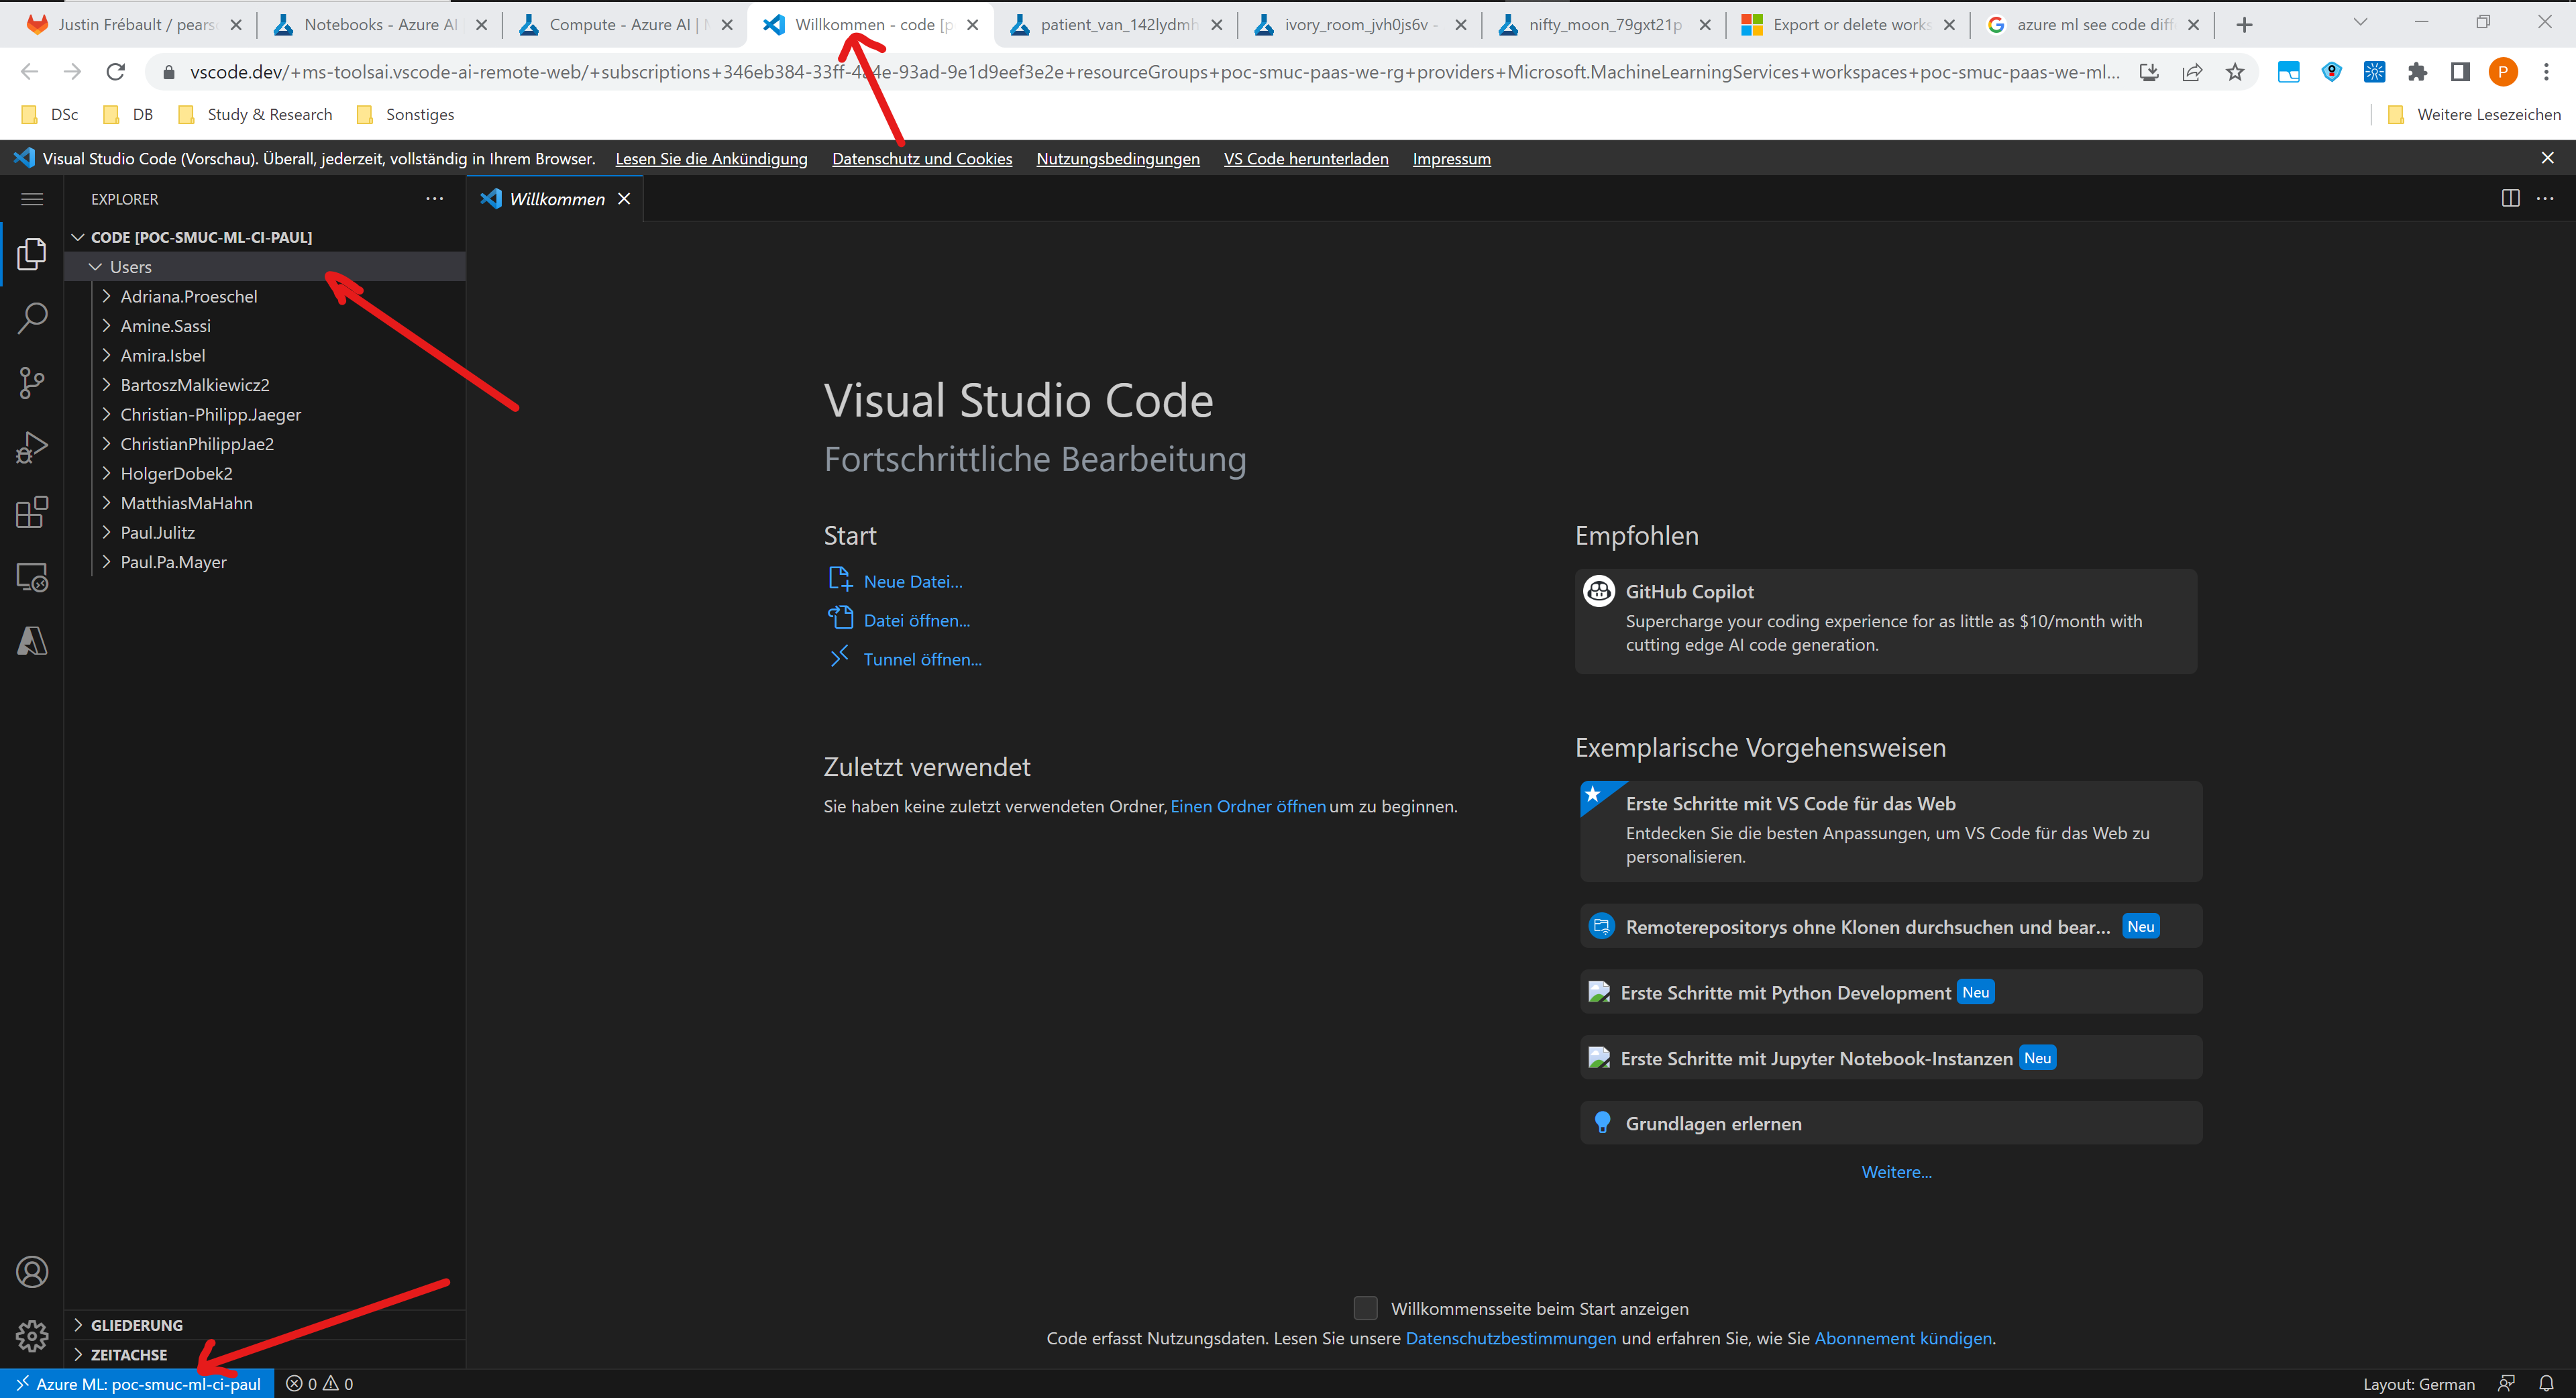
\includegraphics[scale = 0.1]{attachment/chapter_10/Scc049}
	\caption{IDE option: No version controll}
\end{figure}

Either by opening the connection from the compute ressource
 \begin{figure}[H]
 	\centering
 	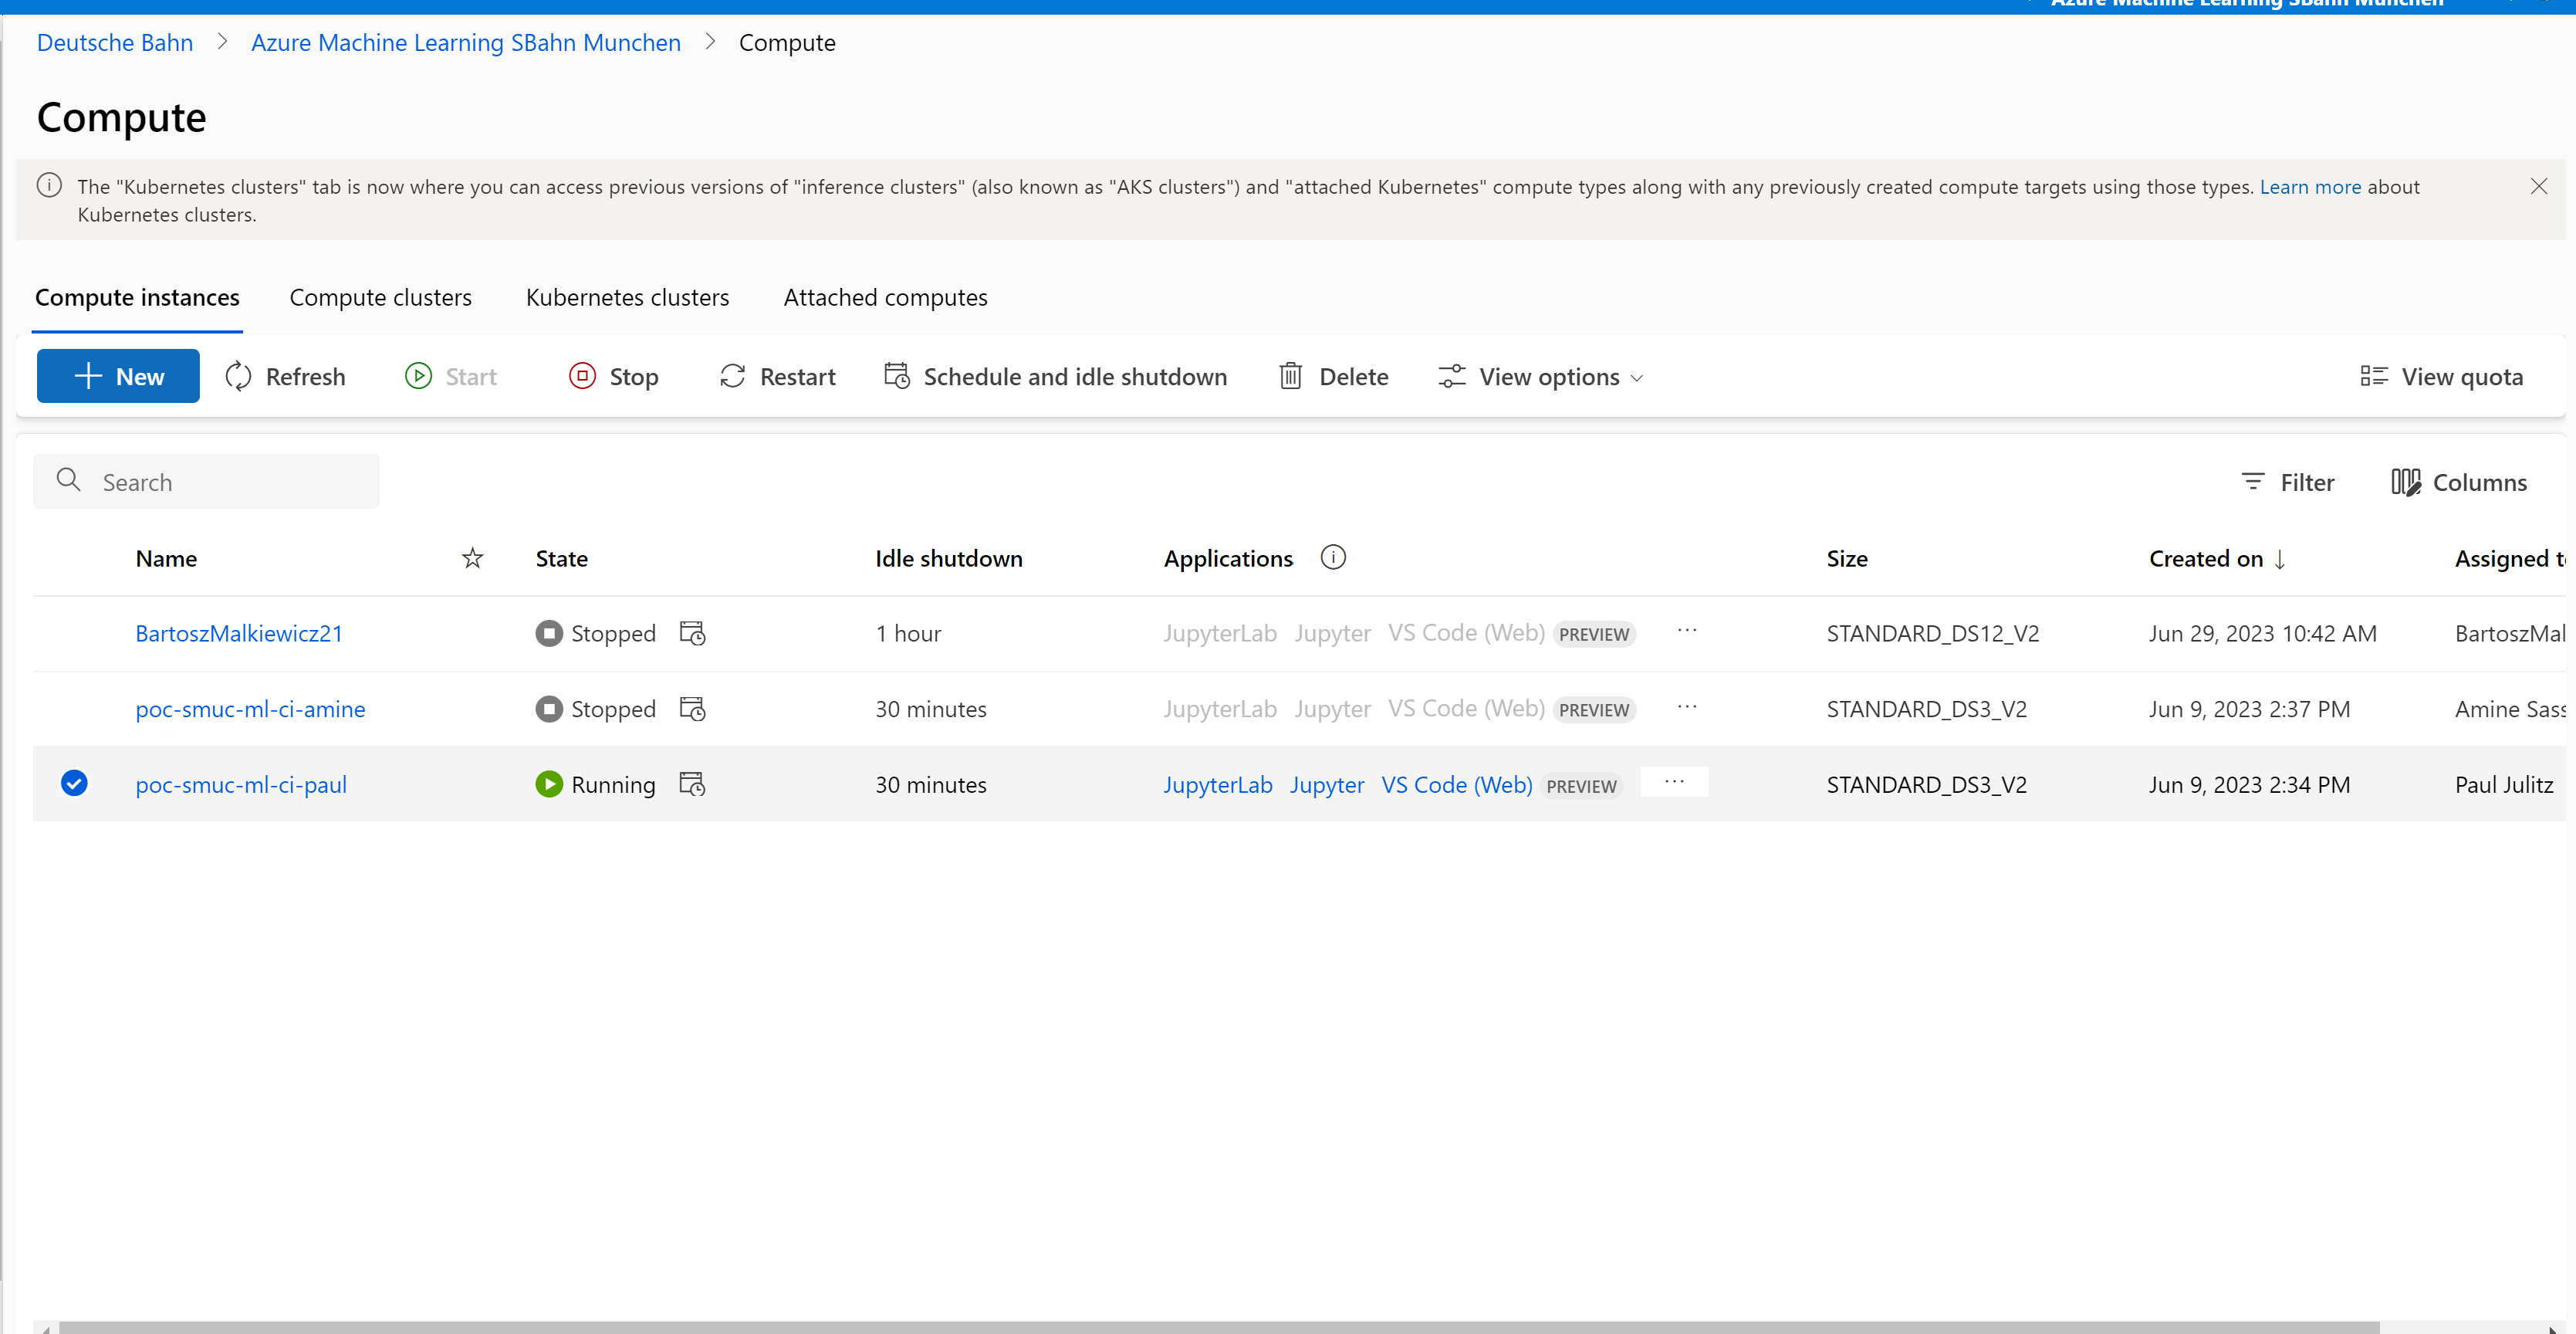
\includegraphics[scale = 0.3]{attachment/chapter_10/Scc046}
 	\caption{Different preview options are available}
 \end{figure}

The files are not versioned.


\subsection{Experiments (Jobs)}

\subsubsection{Creating a Experiment from the Notebook}

The notebook, see \ref{subsub:git_repo}, when executed
\begin{lstlisting}[style=Python]
# Connect to your workspace
import azureml.core
from azureml.core import Workspace

# With Visual Studio Code, the default ws is set up
ws = Workspace.from_config()
print(‚Ready to use Azure ML {} to work with {}‘.format(azureml.core.VERSION, ws.name))	

# Start an Experiment
from azureml.core import Experiment
import pandas as pd

# Set name of the experiment
experiment = Experiment(workspace=ws, name=„pearson-titanic“)

run = experiment.start_logging()
print(„Starting experiment:“, experiment.name)
\end{lstlisting}
will create a job run (experiment run) in a own experiment

\begin{figure}[H]
 	\centering
 	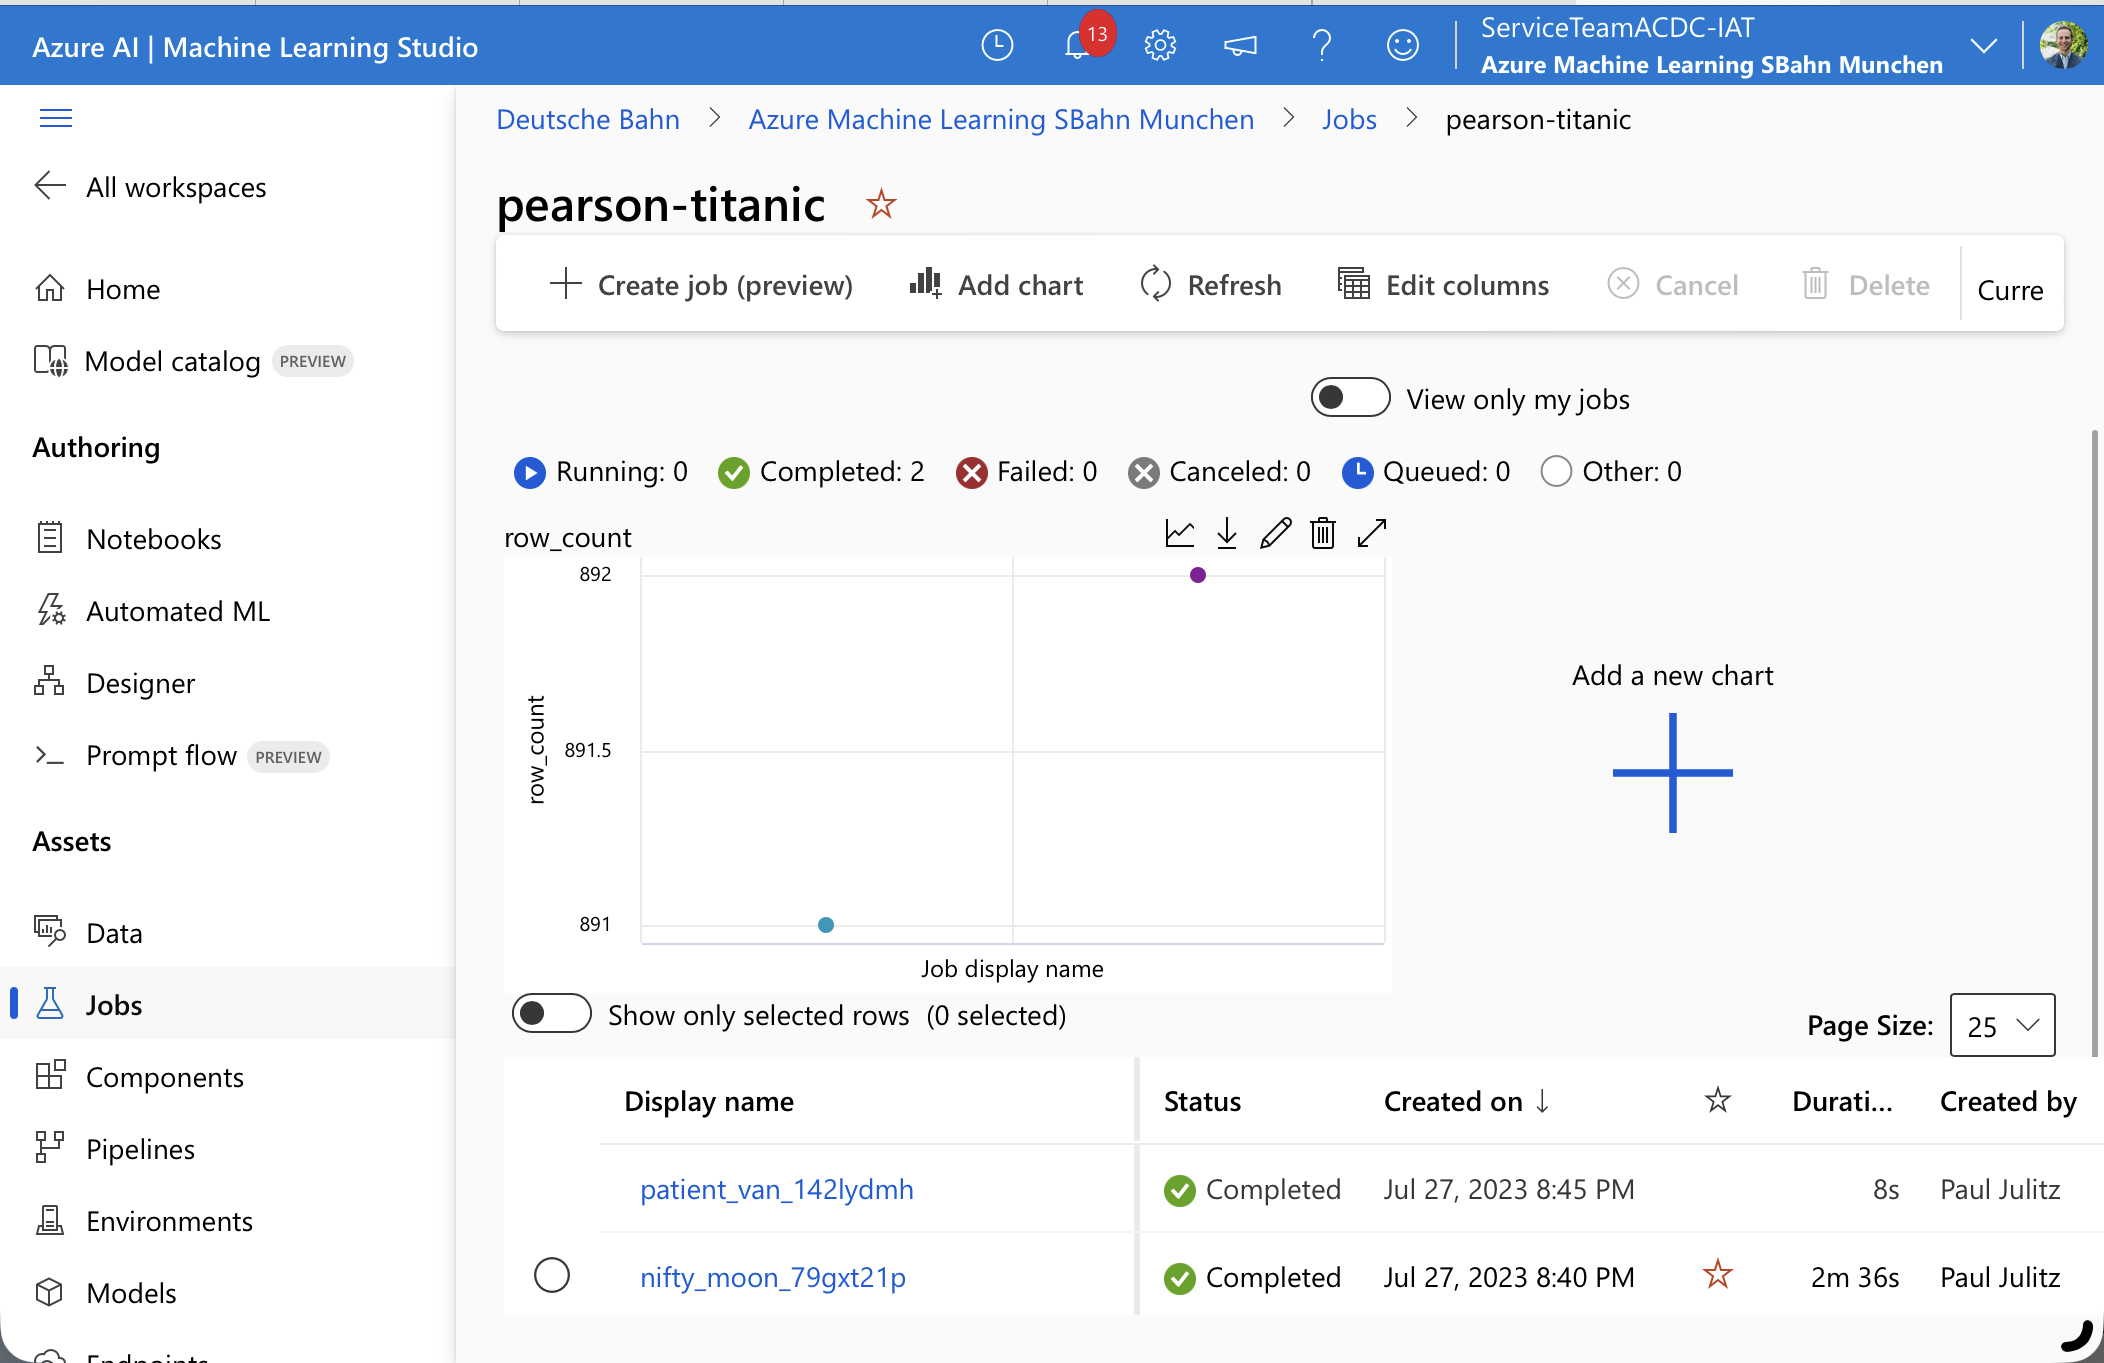
\includegraphics[scale = 0.3]{attachment/chapter_10/Scc050}
 	\caption{Created Experiment}
\end{figure}

With the defined metric, which is logged to the exerimental run, the result are can be seen by the UI in \gls{AML}.

\begin{lstlisting}[style=Python]
	# Read data
	data = 
	pd.read_csv(‚data/titanic.csv‘)
	
	#Count the number of rows and log it as a metric
	row_count = (len(data))
	run.log(‚row_count‘, row_count)
	
	# End experiemnt and query metrics
	run.complete()
	
	print(„Metrics“)
	metrics = run.get_metrics()
	for metric_name in  metrics:
		print(metric_name, „:“, metrics[metics_name]
\end{lstlisting}

\begin{figure}[H]
 	\centering 	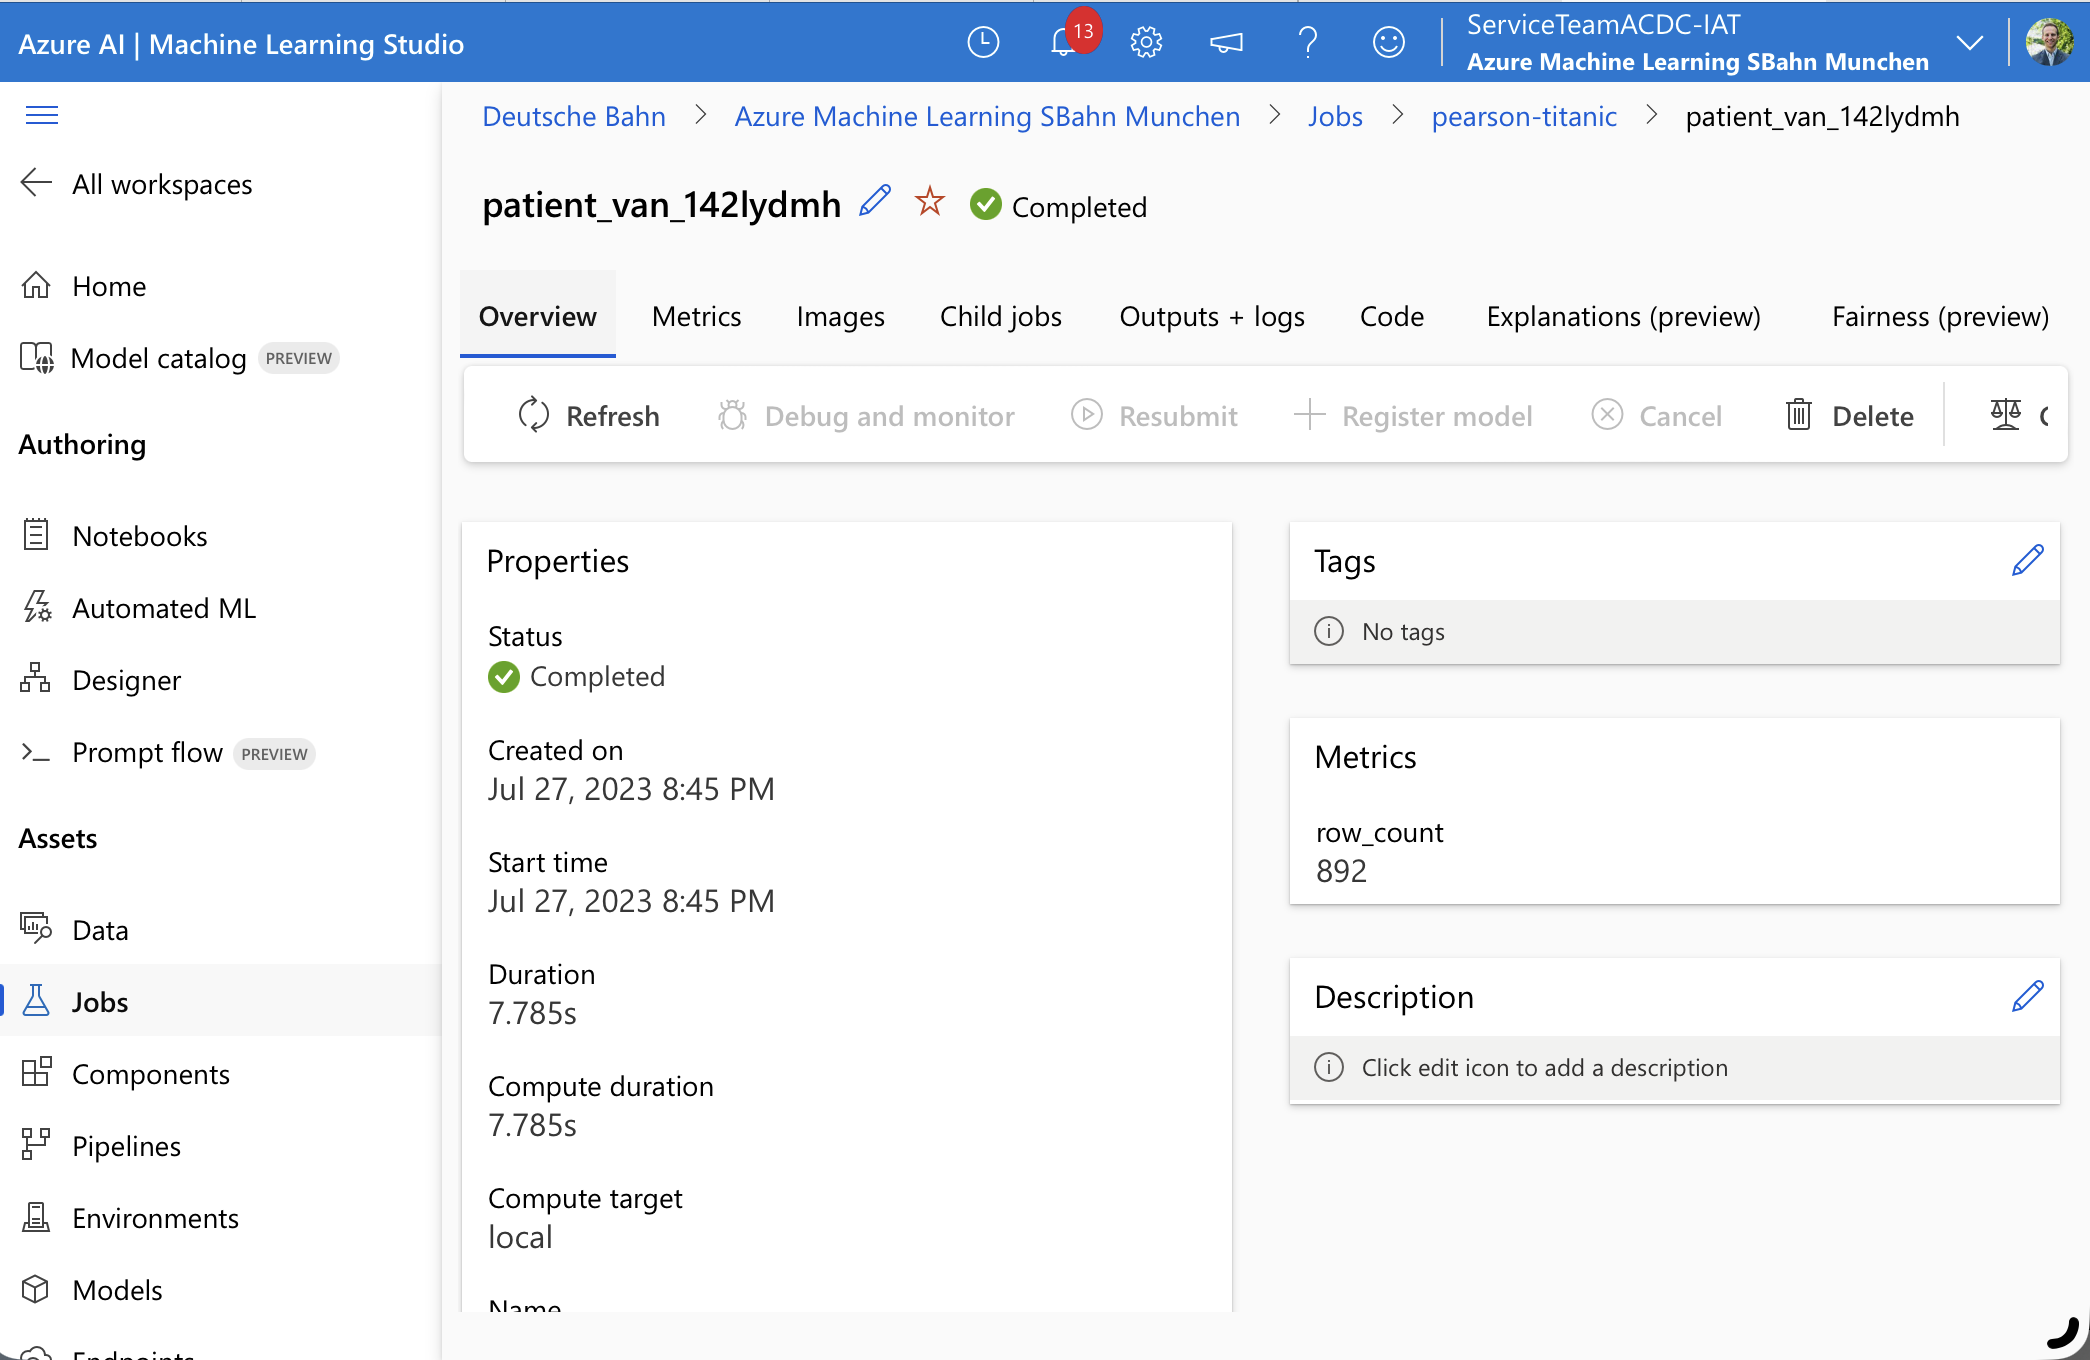
\includegraphics[scale = 0.3]{attachment/chapter_10/Scc051}
 	\caption{Job runs in Azure ML}
\end{figure}


\subsubsection{Overview}

Wenn ein Trainingskript durchgeführt wird, kann der Output und die Metriken zu dieser Durchführung getrackt werden. Das gleiche Experiement kann mehrmal mit verschiedenen 
\begin{itemize}
	\item Hyperparameters,
	\item Trainingsdaten und
	\item Einstellungen 
\end{itemize}
durchgeführt werden. 

Im Arbeitsbereich wird jedes Experiment geloggt mit den Ergebnissen. Diese Logs geben eine Auskunft, den Verlauf eines Modells zu beobachten. Die Änderungen zu verfolgen, welche zu einer Verbesserung geführt haben und wann das Model in Produktion genommen wird.




\section{MLOps for Python models using Azure Machine Learning}

\subsection{Steps in the ML Process}
\paragraph{Aim: Seemless working together}

All models - including those that work perfectly, need
\begin{itemize}
	\item retraining 
	\item and monitoring.
\end{itemize}
The Azure ML Platform provids a \gls{CI}/\gls{CD} experience for machine learning workflow. The capabilities \gls{MLOps}.This allows \textit{ML Engineer} and Data Scientist to work more seemless together. One is designing the model and the other is engineering the deployment and optimizsation.

\paragraph{Data Preparation - Dataset Versoning}
This takes most of the time. Cleaning, getting it shape and having better quality. This process is supported by \textit{Versioning of datasets}. This allows to follow the process of the datasets.

\paragraph{Creating a Model - Experimentation}
To create a model many steps have to be made:
\begin{itemize}
	\item Feature selection,
	\item Algorithmen selection
	\item Fitting the model
	\item Hyperparmeter tuning
\end{itemize}

This process is captured by what is called as \textit{Experimentation}.

\paragraph{Monitoring}
Wenn das Model in der Produktion ist, ist das Monitoring von Relevanz. 

\begin{figure}[H]
	\centering
	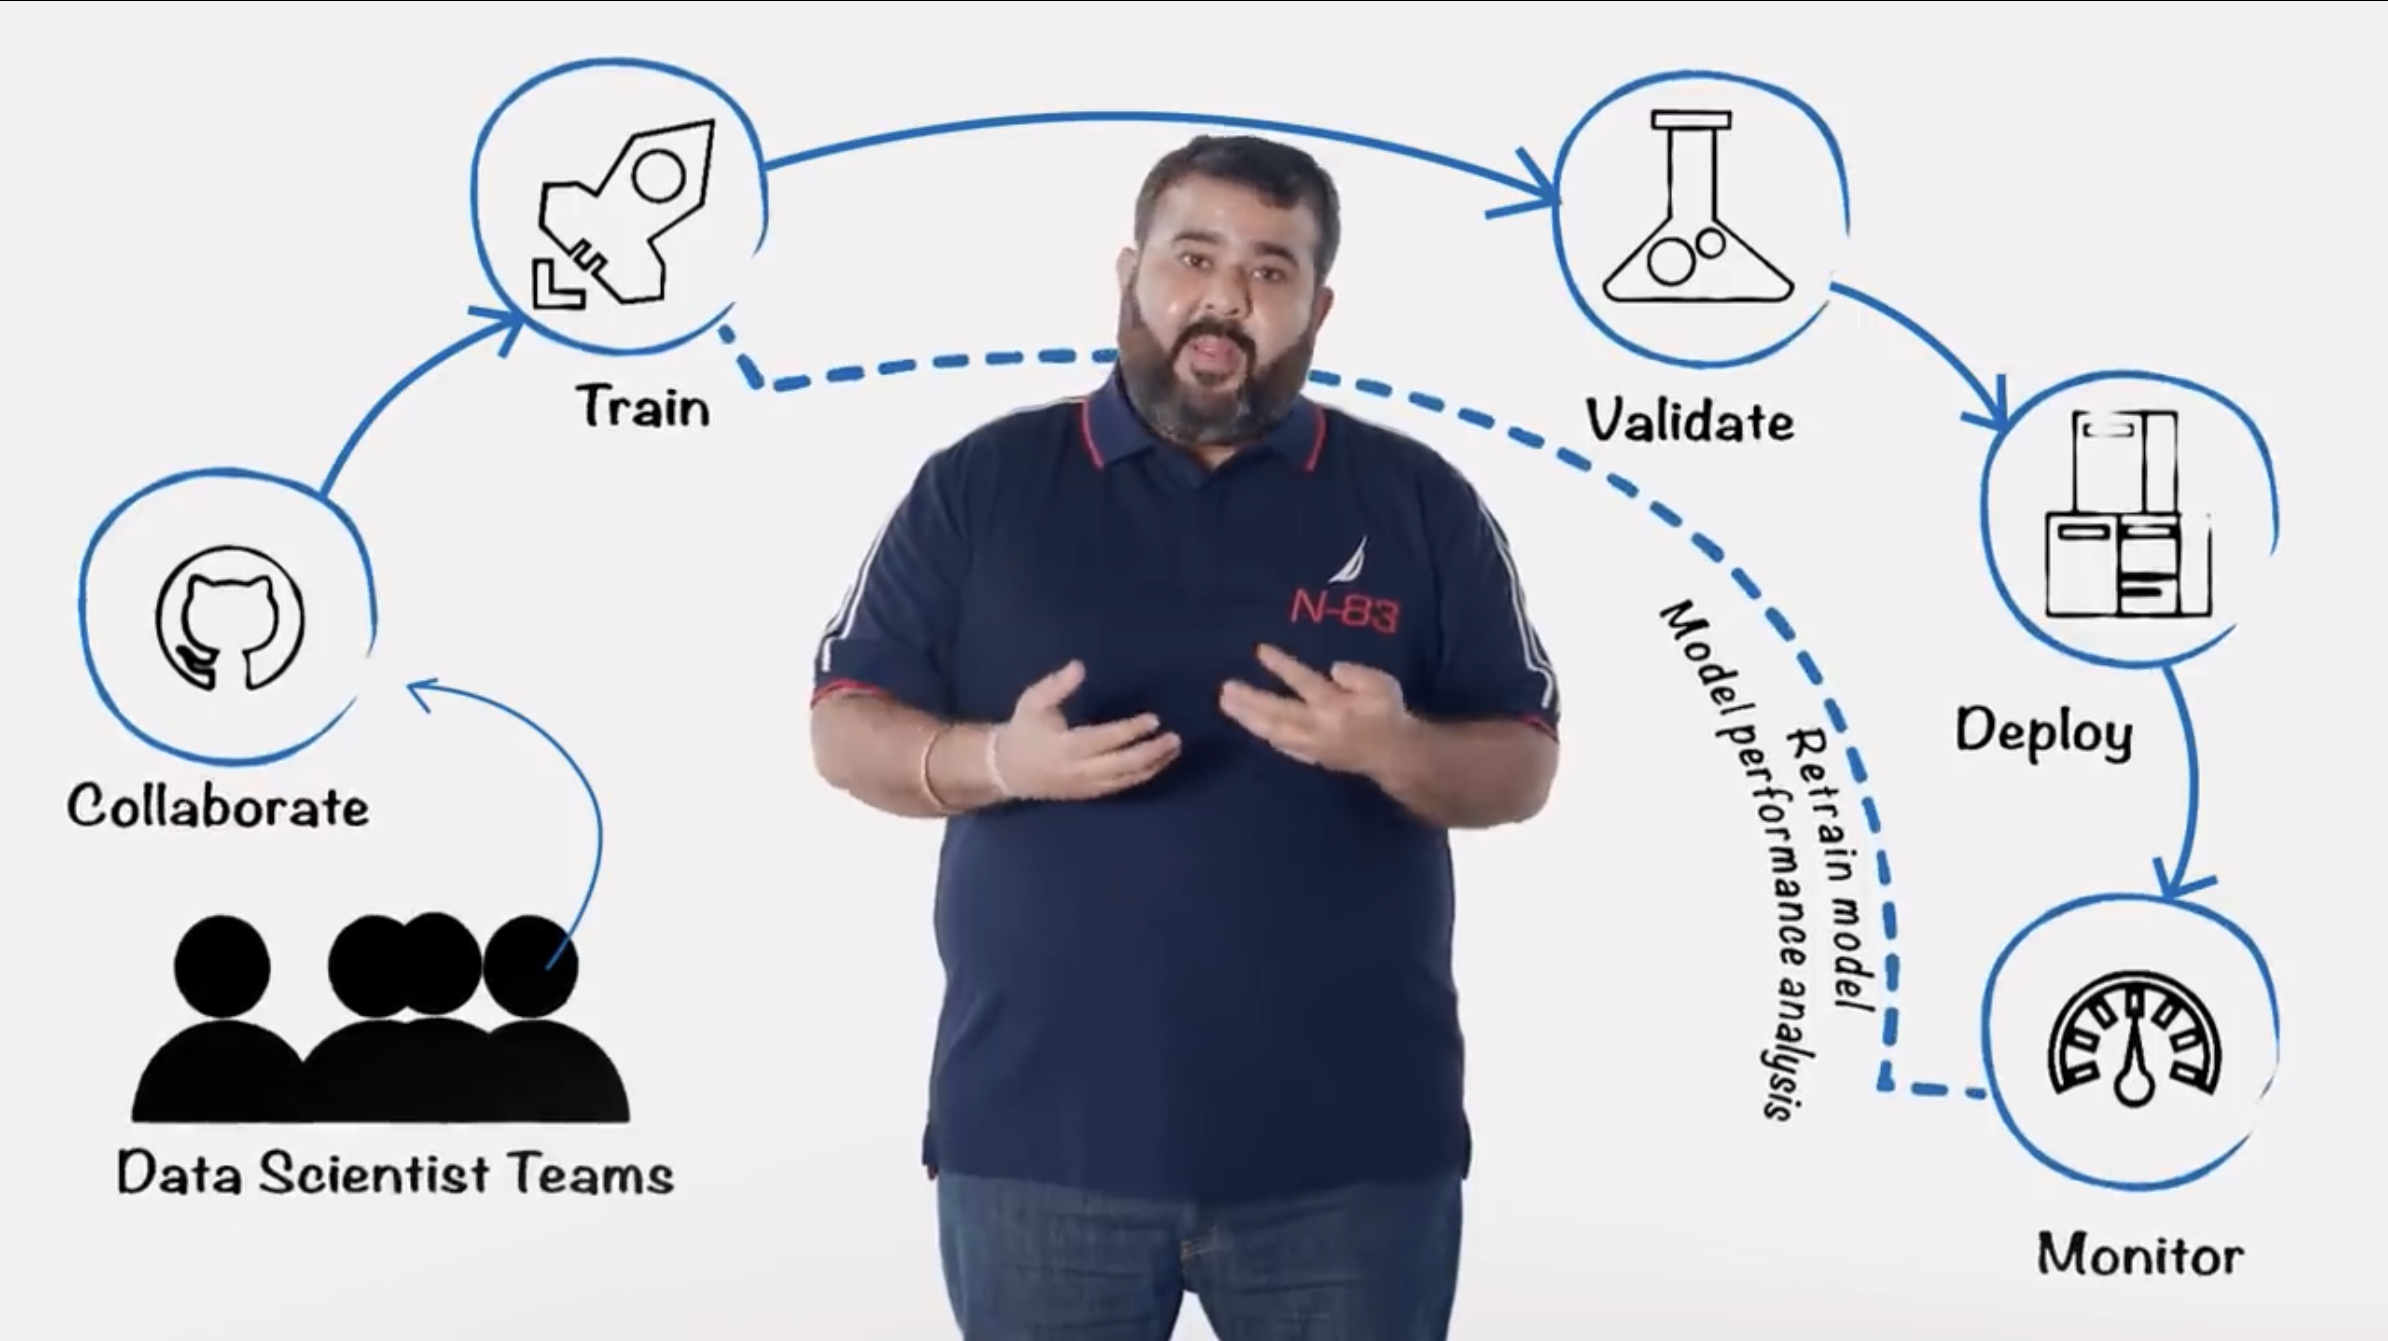
\includegraphics[scale = 0.1]{attachment/chapter_10/Scc025}
	\caption{Monitoring Part in the MLOps Cyclus}
\end{figure}

Es gibt zwei Konzept, welche besonders für den ML Prozess sind:
\begin{description}
	\item[Model Drift] Die geschäftlichen Anforderungen, der Use Case, ändern sich. Das Model muss angepasst werden, weil die Performance sich verschlechtert, weil der Zusammenhang zwischen Input und Output sich geändert haben.
	\begin{figure}[H]
	\centering
	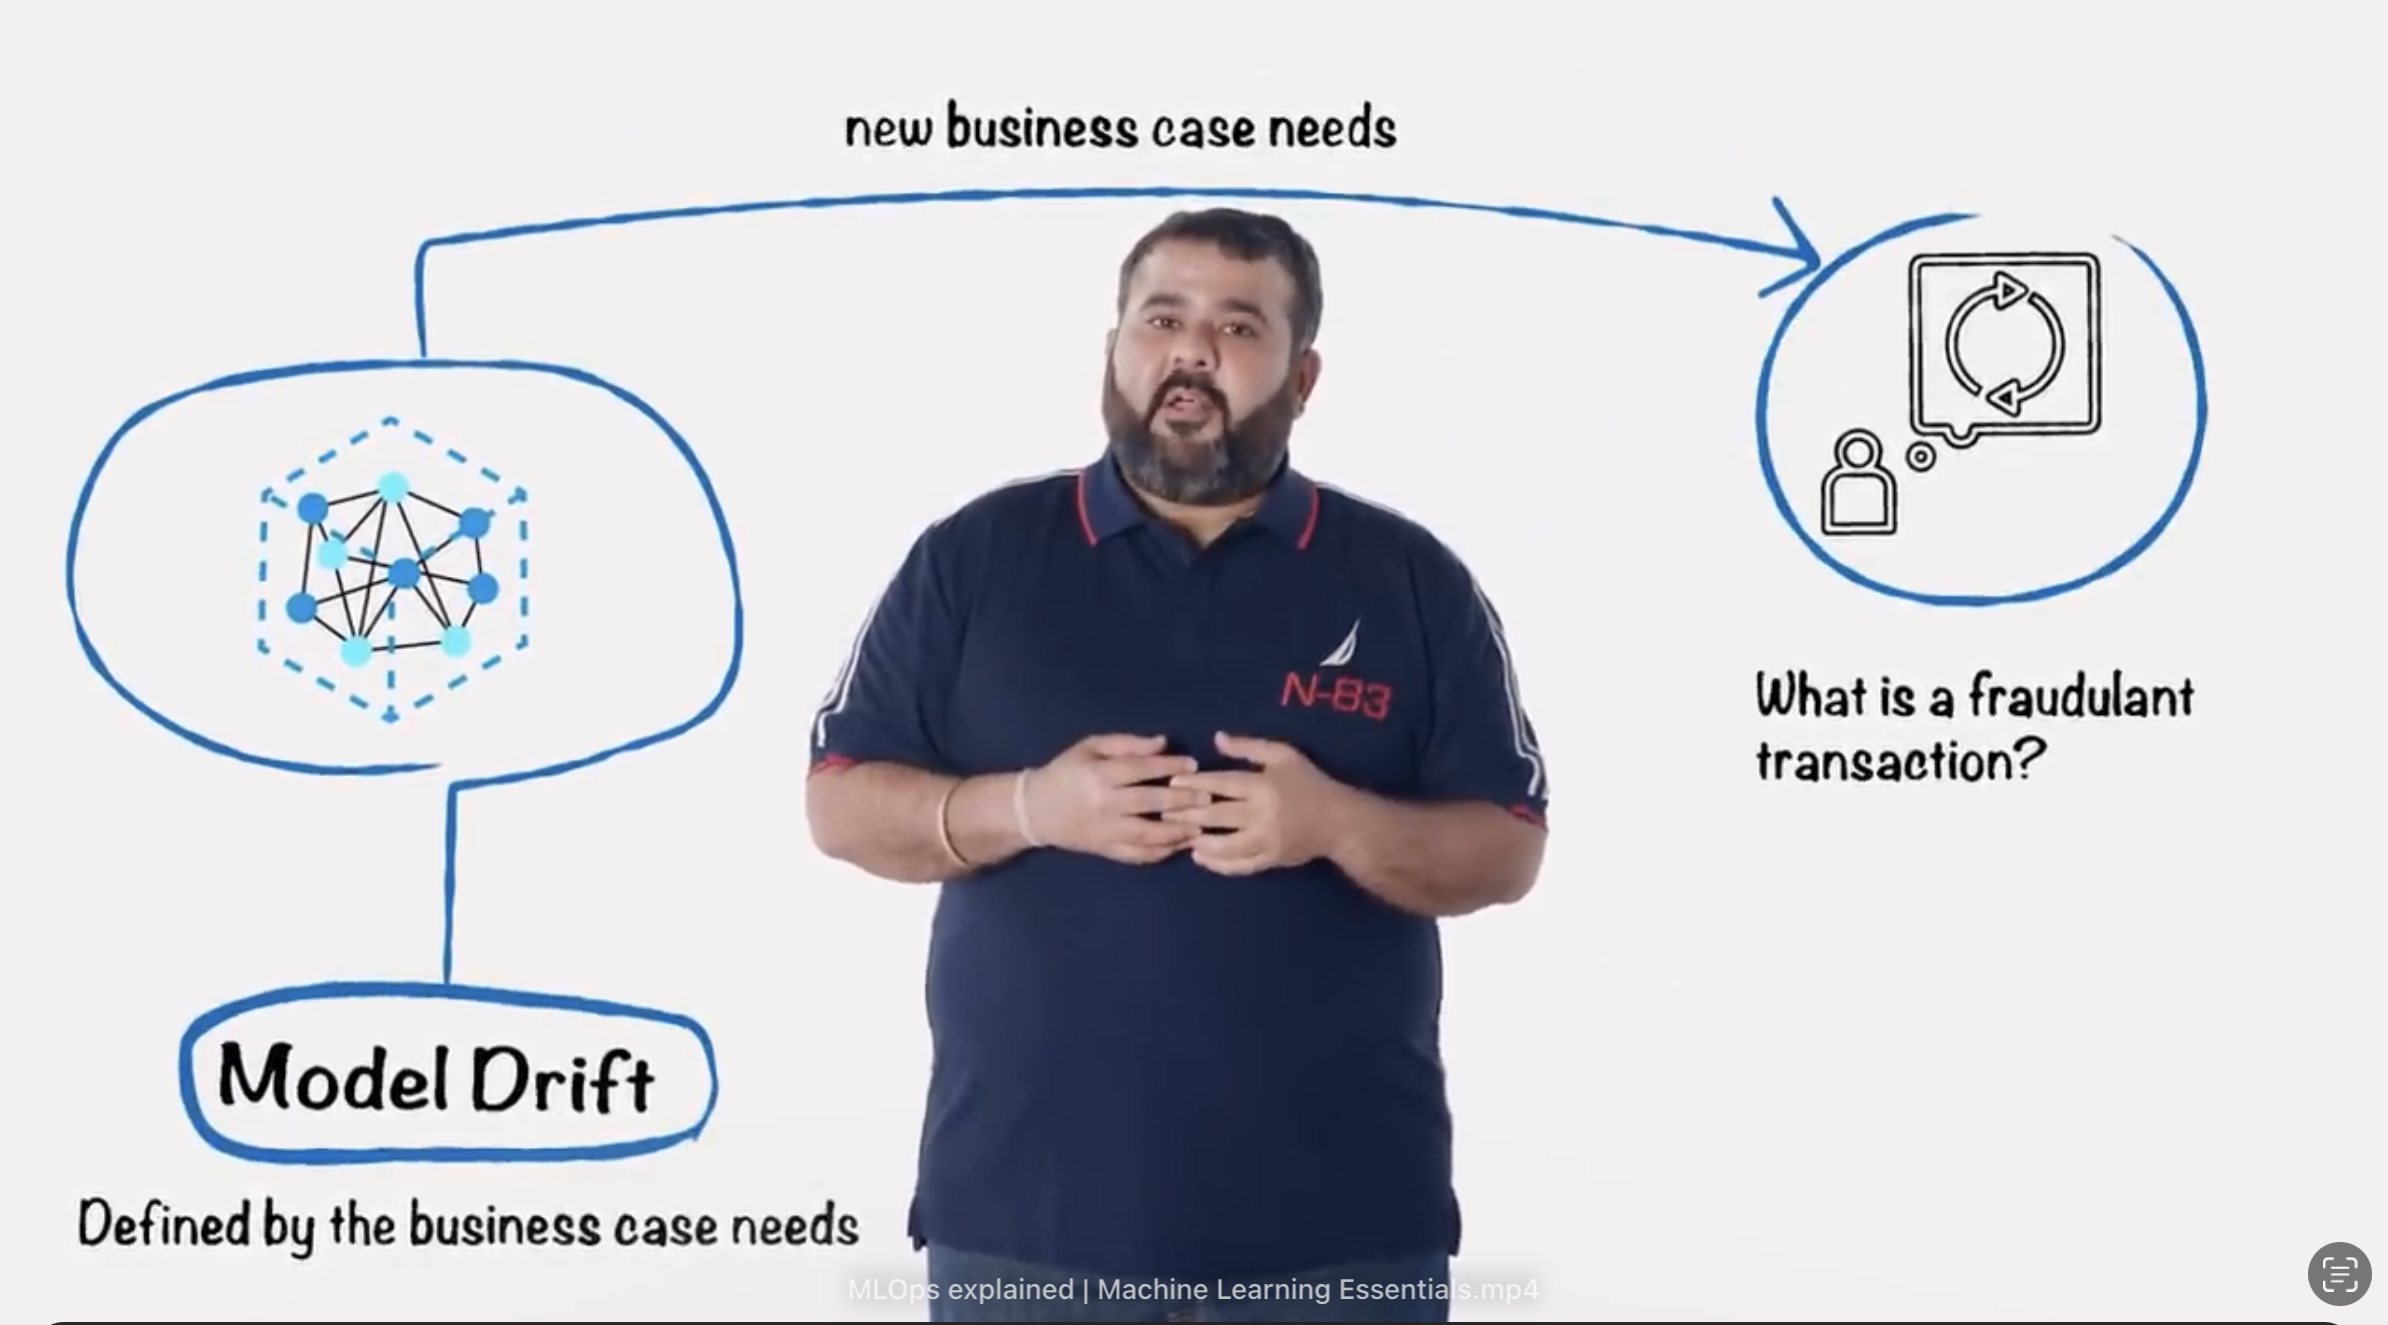
\includegraphics[scale = 0.1]{attachment/chapter_10/Scc027}
	\caption{Example: Different Buisnes Definitions}
\end{figure}
	\item[Data Drift] Zusammenhänge in den Daten ändern sich: Bsp.: Sainalität, Geschlecht. Die Stichprobe entspricht nicht mehr der Verteilung, aus welcher das Model gebildet wurde.
	\begin{figure}[H]
	\centering
	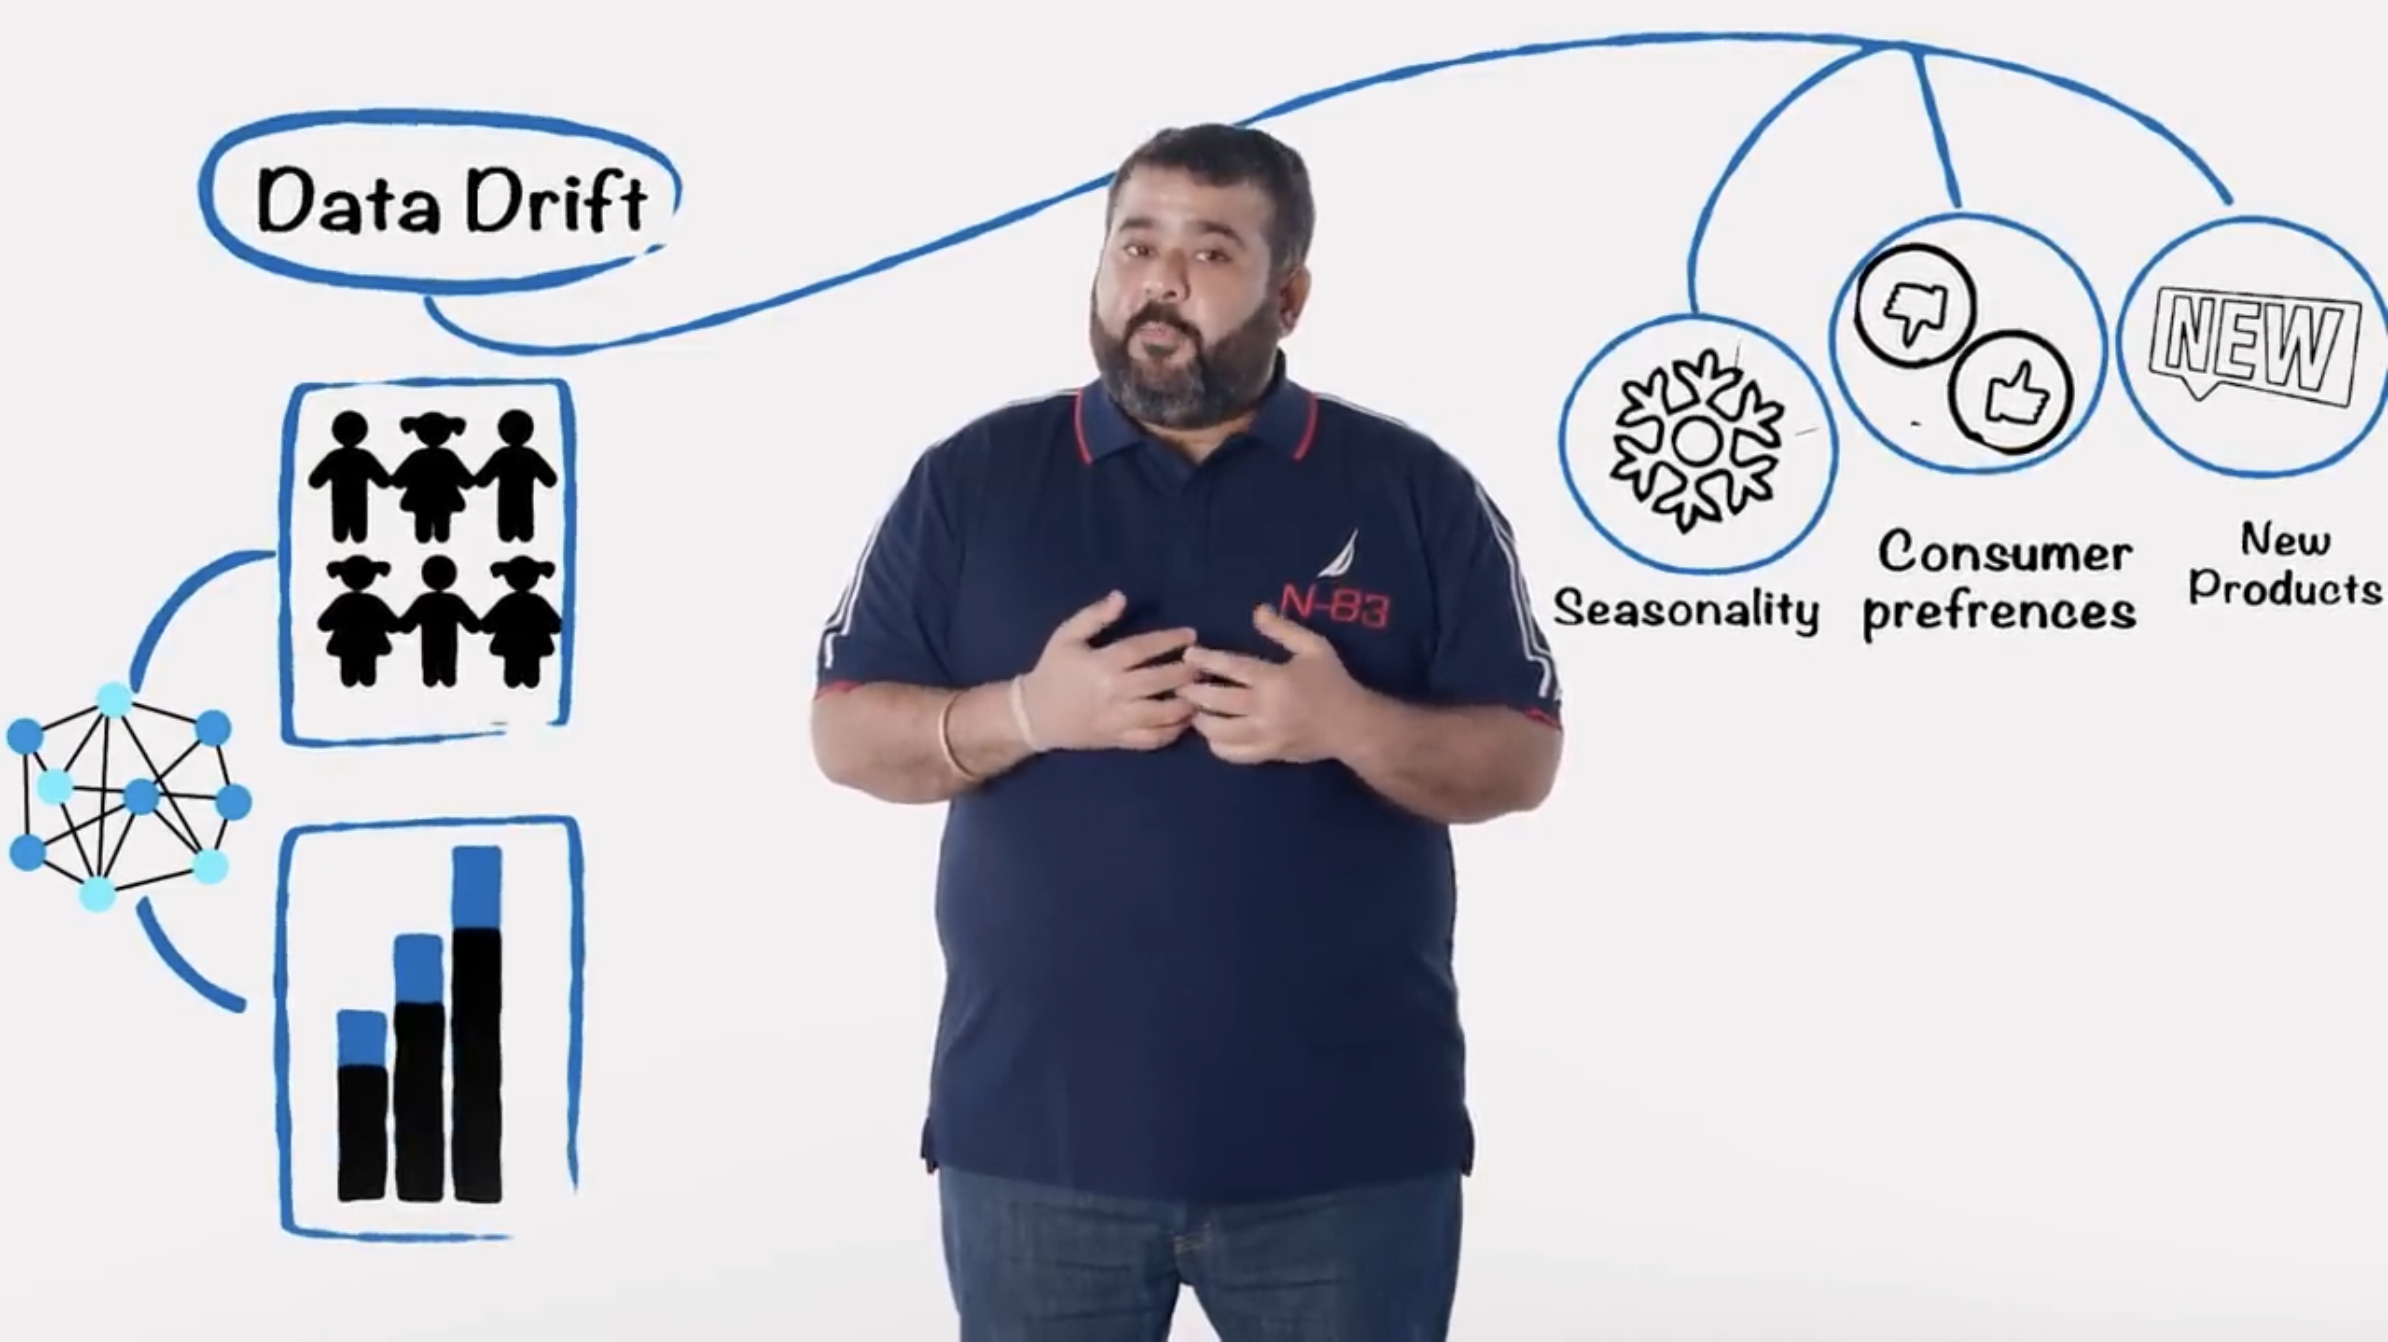
\includegraphics[scale = 0.1]{attachment/chapter_10/Scc026}
	\caption{Examples: Different sample distribution; Seasonality}
\end{figure}
\end{description}




\subsection{CI/CD Process}
\paragraph{Build Pipeline}

With \textit{Azure DevOps} the Testing-Part and setting up required configuration can be done. The \gls{SDK} allows to interact with the components of \textit{Azure ML}. 


\begin{figure}[H]
	\centering
	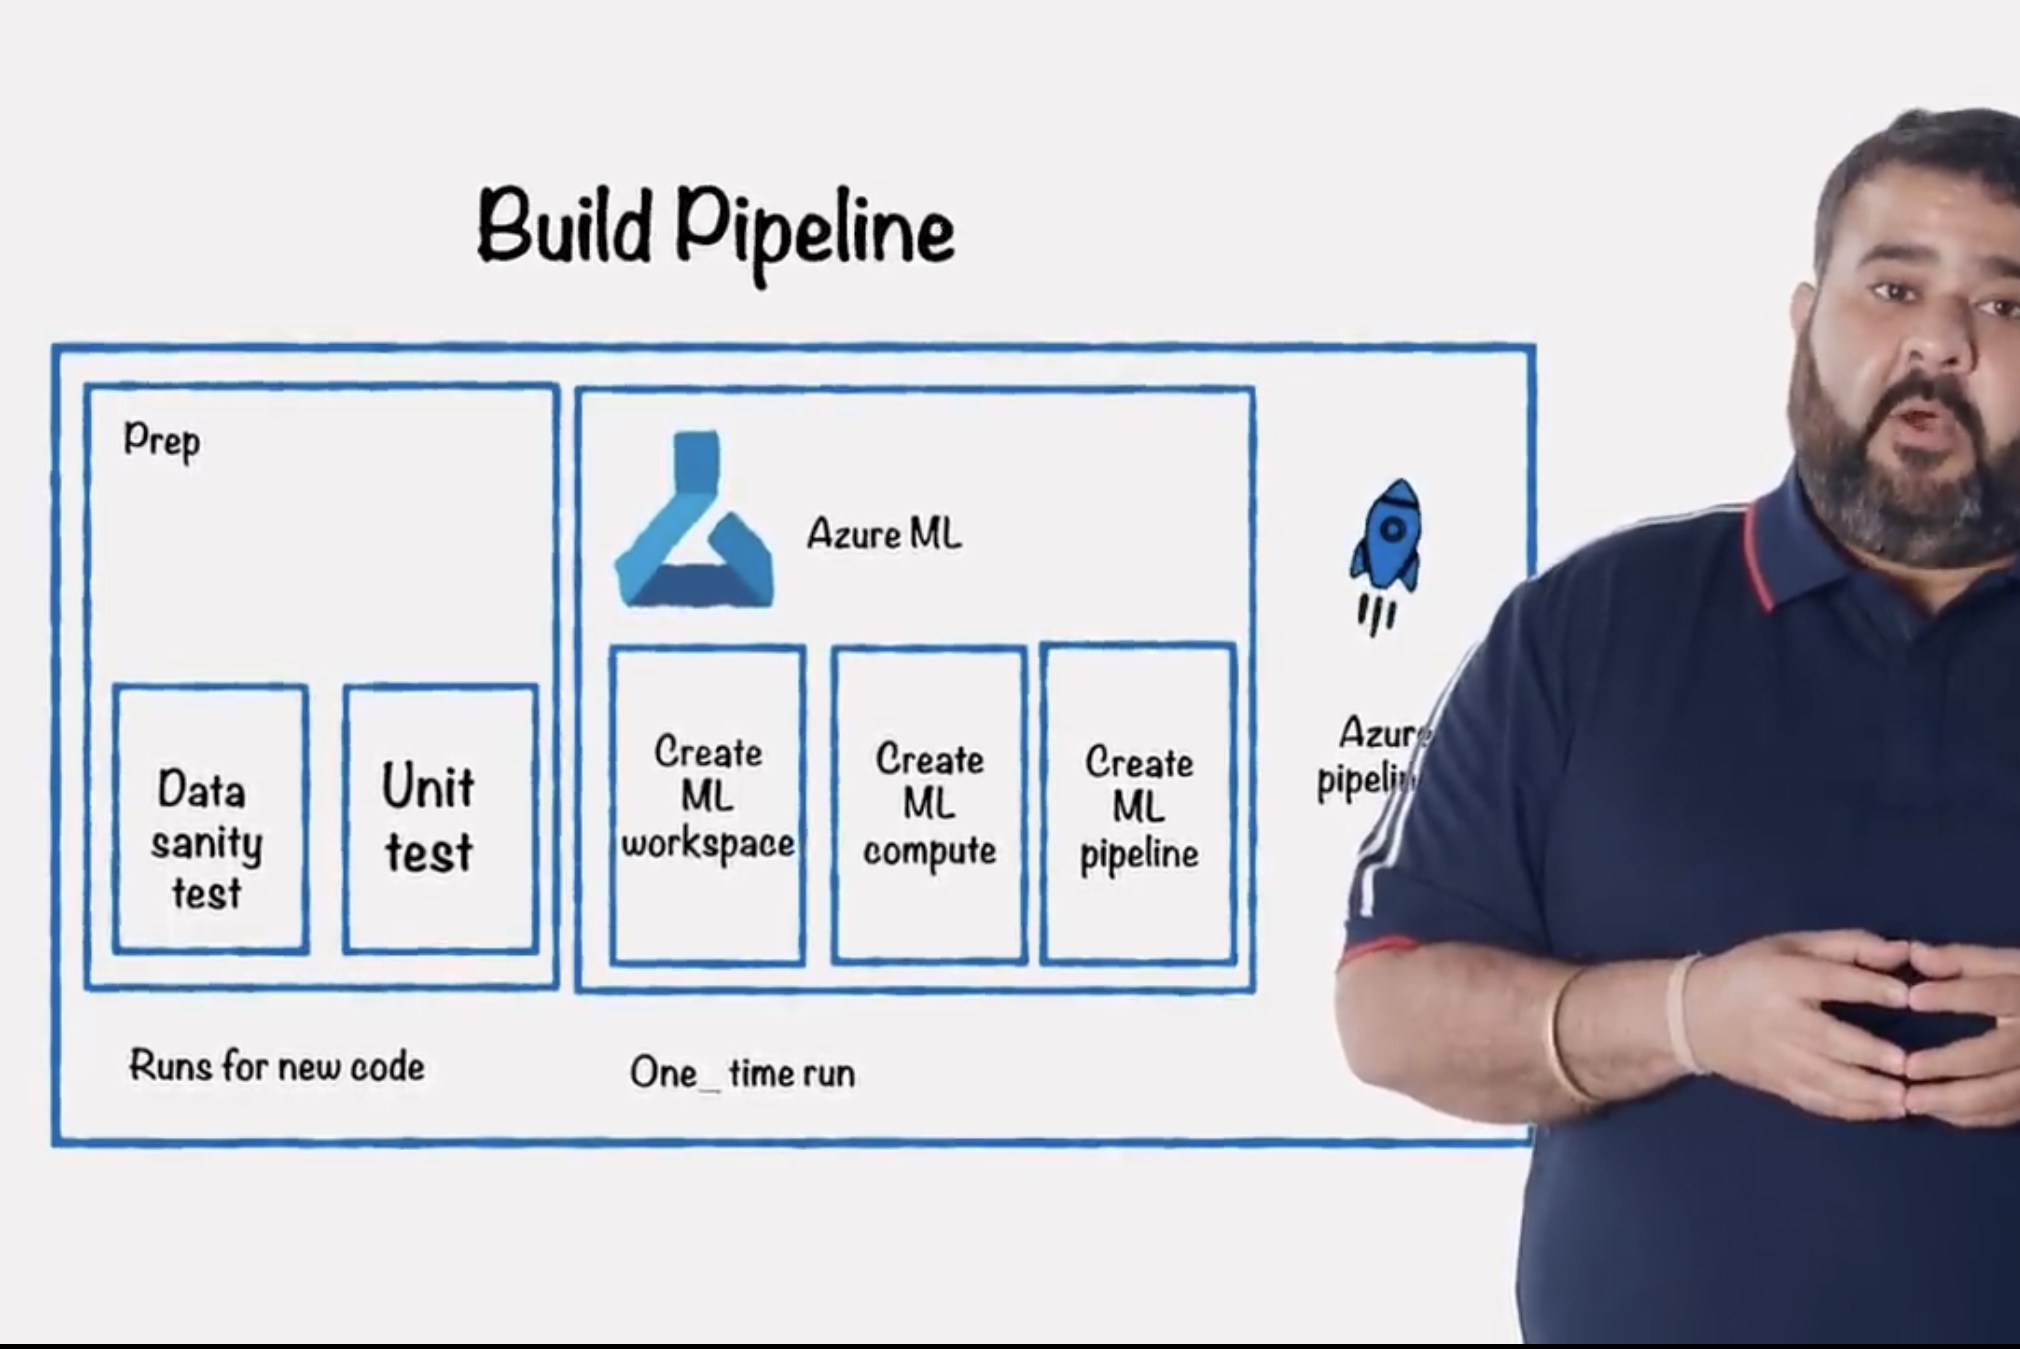
\includegraphics[scale = 0.1]{attachment/chapter_10/Scc020}
	\caption{Once and continuous Build}
\end{figure}

This build pipeline creates once an workspace, compute instances and a pipeline in with a model lives.\\

This architecture is also a setup, for a relativly normal \gls{CI} process. This process works, when you use a repository to change parts in \textit{Azure ML}. \underline{Caution:} The process is different in Azure Synapse Analytics then in Azure ML. In Azure ML the \gls{SDK} gives you a way to interact with the components.

\begin{figure}[H]
	\centering
	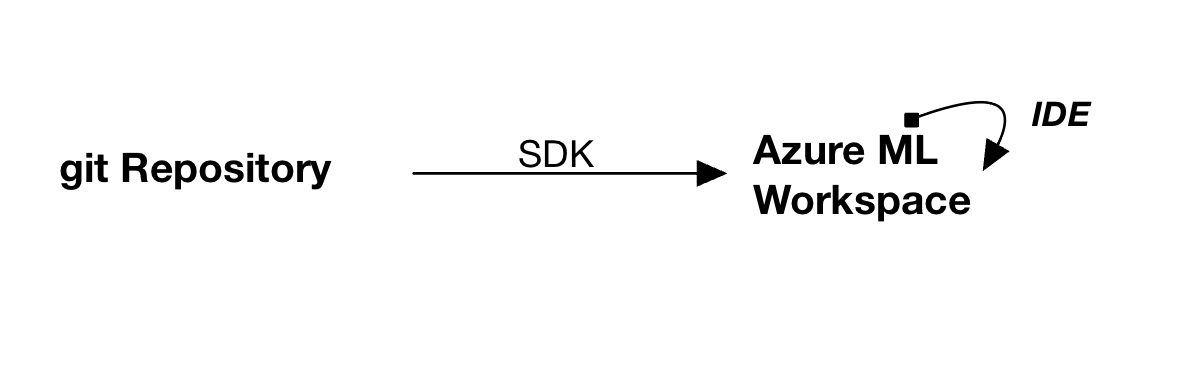
\includegraphics[scale = 0.3]{attachment/chapter_10/Scc021}
	\caption{Interaction with Azure ML}
\end{figure}

In Synapse the hole template for interacting with the ressources can be changed in the repository or vise versa over the \gls{IDE}.

\begin{figure}[H]
	\centering
	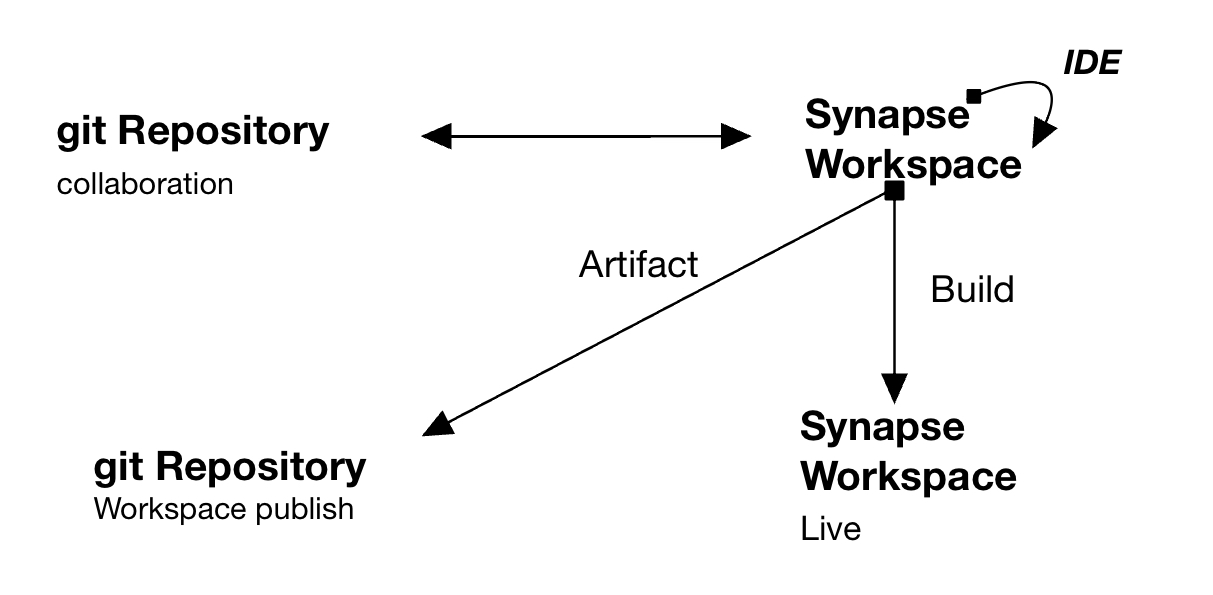
\includegraphics[scale = 0.3]{attachment/chapter_10/Scc022}
	\caption{Interaction with Synapse}
\end{figure}

\paragraph{Retraining Pipeline}

A Azure ML pipeline are reusable workloads. This is can also be use to retrain models. This can be triggered, when a new data is available. With Azure DevOps pipeline can this trigger be identify and the pipeline in Azure Ml be triggered.\\

The retraining steps can include
\begin{itemize}
	\item train on new data
	\item evaluate the new model
	\item and if the efficacy is reached, a new version of the model can be regristered.
\end{itemize}

\begin{figure}[H]
	\centering
	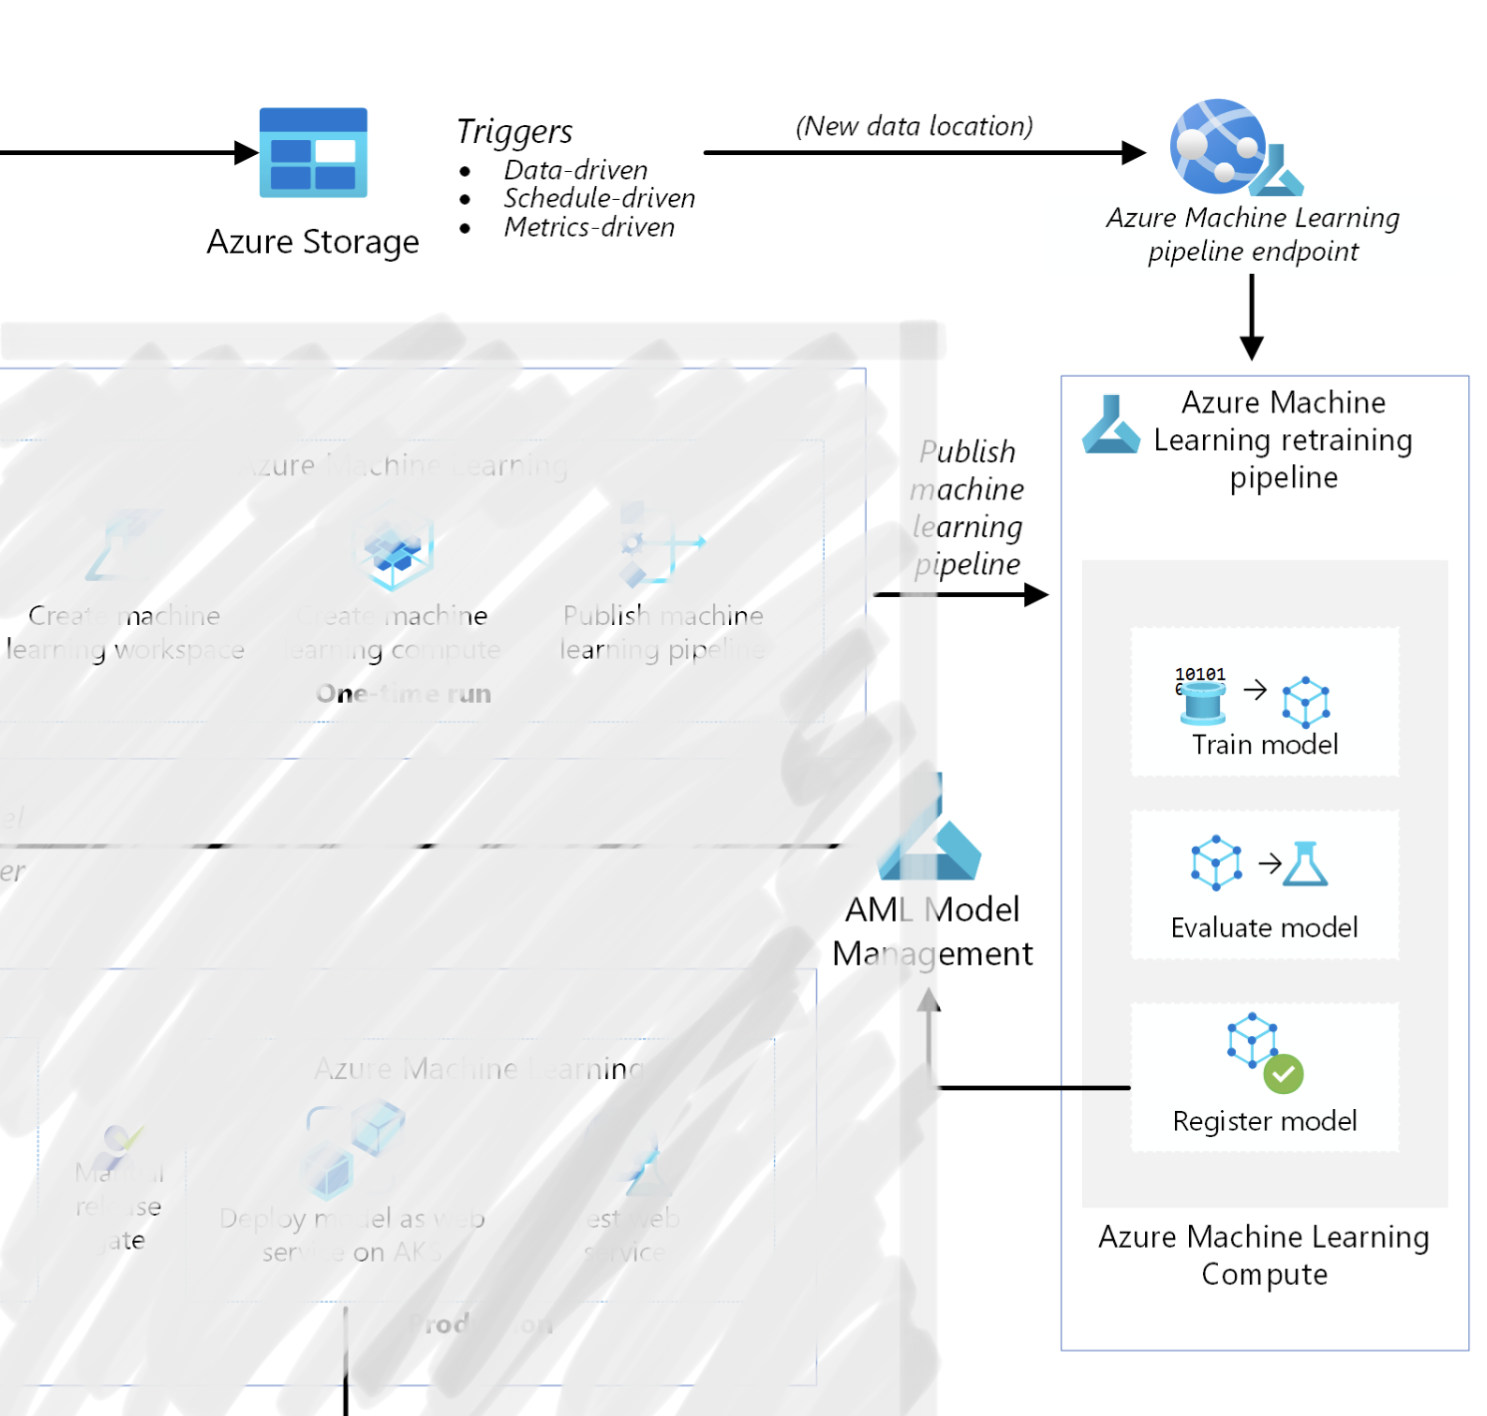
\includegraphics[scale = 0.2]{attachment/chapter_10/Scc023}
	\caption{Example Retraining Pipeline}
\end{figure}

\paragraph{Release Pipeline}
With Azure DevOps Release Pipeline the model gets
\begin{itemize}
	\item page model to and image image,
	\item deploy it to and web service enpoint. 
\end{itemize}
This can be done combined with \textit{managed endpoints}. The webservice in then hosted on a \gls{ACI} for the \textit{Q and A process}. For production load a \gls{AKS} is normally deployed.

\begin{comment}
	


\section{*Azure Machine Learning SDK}
Azure provides a \gls{SDK} for Python and \gls{R} to interact with the services of \gls{AML} in different enviorments.

\begin{figure}[H]
	\centering
	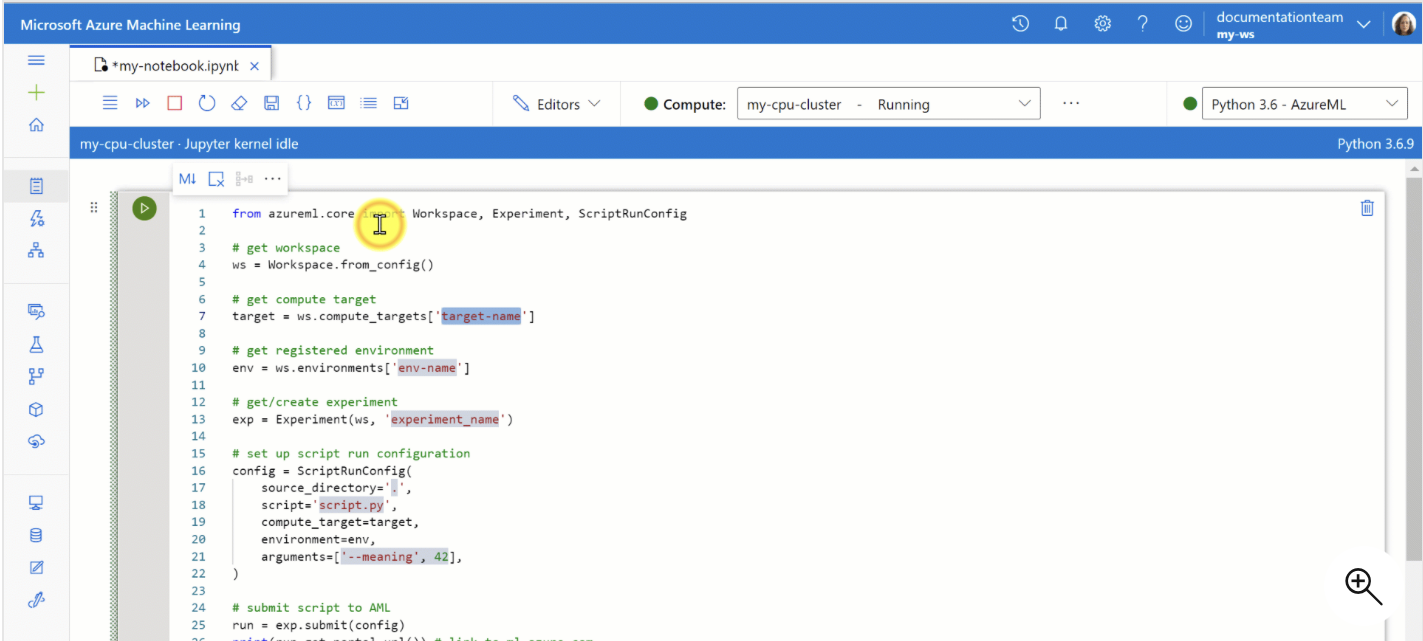
\includegraphics[scale = 0.4]{attachment/chapter_10/Scc003}
	\caption{Crt + Space - IntelSense}
\end{figure}

	\paragraph{Framework agnostic}
%TODO: OLD Unclear how to use it.
Over this platform 
\begin{itemize}
	\item Scikit-learn, 
	\item Tenserflow, 
	\item \gls{g_ONNX},
	\item MLFlow,
	\item PyTorch
\end{itemize}

\end{comment}
